\documentclass[12pt, bibliography=totoc, a4paper, abstractoff, numbers=noenddot]{scrreprt}

% define used packages
\usepackage[left=4.0cm, right=2.0cm, top=3cm, bottom=3cm]{geometry}
\usepackage{bibgerm}
\usepackage[utf8]{inputenc}
\usepackage[T1]{fontenc}
\usepackage{graphicx}
\usepackage[ngerman]{babel}
\usepackage{lmodern}
\usepackage{listings}
\usepackage{amsthm}
\usepackage{lstautogobble}
%\usepackage{amssymb}
\newtheorem*{definition}{Definition}
\usepackage[numbers]{natbib}
\usepackage{acronym}
\usepackage{enumitem}
\usepackage{multirow}

\bibliographystyle{alphadin}
\usepackage{float}

\usepackage{lastpage}

% advanced tables
\usepackage{array}

% header and footer
\usepackage{fancyhdr}

% links
\usepackage{url}

% internal links
\usepackage[colorlinks=true ,linkcolor=black,
			anchorcolor=black ,citecolor=black ,filecolor=black,
			menucolor=black ,urlcolor=black]{hyperref}

% mathematical formulas
\usepackage{amsmath, amssymb}

% fancy Diagrams %
\usepackage{tikz}
\usepackage{epstopdf}

% to include images side by side
\usepackage{subfigure}

% for nice bg on title page
\usepackage{eso-pic}
\newcommand\BackgroundPic{%
\put(0,0){%
\parbox[b][\paperheight]{\paperwidth}{%
\vfill
\centering

\includegraphics[width=\paperwidth,height=\paperheight,%
keepaspectratio]{images/Logo_H-BRS_background}pdf}%
\vfill
}}

%\usepackage{caption}

% define the programming language
\usepackage{listings}
\lstloadlanguages{Java,sh,bash,Haskell,HTML,PHP,XML}
\lstdefinelanguage{console}{
  morekeywords={},
  otherkeywords={warumgehtdasnicht>,\$}
}
\newcommand{\lstsetconsole}
{ \lstset{%language=sh,
        lineskip=-2pt,
        breaklines=true,
        language=console,
        breaklines=true,
        captionpos=b,
        commentstyle=\textit,
        keywordstyle=\bfseries,
        basicstyle=\ttfamily,
        stringstyle=\ttfamily,
        showstringspaces=false,
        frame=single,
        tabsize=2
  }
}
\lstdefinelanguage{scalaconsole}{
  morekeywords={},
  otherkeywords={scala>,\|}
}
\newcommand{\lstsetrepl}
{ \lstset{%language=sh,
        lineskip=-2pt,
        breaklines=true,
        language=scalaconsole,
        breaklines=true,
        commentstyle=\textit,
        keywordstyle=\bfseries,
        basicstyle=\ttfamily,
        stringstyle=\ttfamily,
        showstringspaces=false,
        frame=single,
        tabsize=2
  }
}
\newcommand{\lstsetjava}{
 \lstset{language=Java,
        breaklines=true,
        commentstyle=\textit,
        keywordstyle=\bfseries,
        basicstyle=\ttfamily,
        stringstyle=\ttfamily,
        showstringspaces=false,
        frame=single,
        captionpos=b,
        tabsize=2,
        literate=
        %linewidth=\textwidth,captionpos=b
        %numbers=left, stepnumber=5, numbersep=10pt
 }
}
\lstdefinelanguage{scala}{
  morekeywords={abstract,case,catch,class,def,%
    do,else,extends,false,final,finally,%
    for,forSome,if,implicit,import,lazy,match,mixin,%
    new,null,object,override,package,%
    private,protected,requires,return,sealed,%
    super,this,throw,trait,true,try,%
    type,val,var,while,with,yield},
  otherkeywords={_,:,=,=>,<-,<\%,<:,>:,\#,@},
  sensitive=true,
  morecomment=[l]{//},
  morecomment=[n]{/*}{*/},
  morestring=[b]",
  morestring=[b]',
  morestring=[b]"""
}
\newcommand{\lstsetscala}{
 \lstset{language=scala,
        breaklines=true,
        commentstyle=\textit,
        keywordstyle=\bfseries,
        basicstyle=\ttfamily,
        stringstyle=\ttfamily,
        showstringspaces=false,
        frame=single,
        tabsize=2
        %%linewidth=\textwidth,captionpos=b
        %numbers=left, stepnumber=5, numbersep=10pt
 }
}
\newcommand{\lstsethtml}{
 \lstset{language=HTML,
        breaklines=true,
        commentstyle=\textit,
        keywordstyle=\bfseries,
        basicstyle=\ttfamily,
        stringstyle=\ttfamily,
        showstringspaces=false,
        frame=single,
        tabsize=2
        %%linewidth=\textwidth,captionpos=b
        %numbers=left, stepnumber=5, numbersep=10pt
 }
}
\newcommand{\lstsetphp}{
 \lstset{language=PHP,
        breaklines=true,
        commentstyle=\textit,
        keywordstyle=\bfseries,
        basicstyle=\ttfamily,
        stringstyle=\ttfamily,
        showstringspaces=false,
        frame=single,
        tabsize=2
        %%linewidth=\textwidth,captionpos=b
        %numbers=left, stepnumber=5, numbersep=10pt
 }
}
\lstnewenvironment{code}
    {\lstset{}%
      \csname lst@SetFirstLabel\endcsname}
    {\csname lst@SaveFirstLabel\endcsname}
\newcommand{\lstsethaskell}{
    \lstset{
      language=Haskell,
      commentstyle=\textit,
      keywordstyle=\bfseries,
      basicstyle=\ttfamily,
      stringstyle=\ttfamily,
      showstringspaces=false,
      frame=single,
      flexiblecolumns=false,
      basewidth={0.5em,0.45em},
      literate={+}{{$+$}}1 {/}{{$/$}}1 {*}{{$*$}}1 {=}{{$=$}}1
               {==}{{$==$}}2 %{!=}{{$\not\equiv$}}2
               {>}{{$>$}}1 {<}{{$<$}}1 {\\}{{$\lambda$}}1
               {\\\\}{{\char`\\\char`\\}}1
               {->}{{$\rightarrow$} }2 {>=}{{$\geq$}}2 {<-}{{$\leftarrow$}}2
               {<=}{{$\leq$}}2 {=>}{{$\Rightarrow$} }2
               {\ .}{{$\circ$}}2 {\ .\ }{{$\circ$}}2 {(.)}{({$\circ$})}2
               {>>}{{>>}}2 {>>=}{{>>=}}2
               {|}{{$\mid$}}1
    }
}
\lstdefinelanguage{JavaScript}{
  keywords={typeof, new, true, false, catch,%
    function, return, null, catch, switch, var,%
    if, in, while, do, else, case, break},
  ndkeywords={class, export, boolean, throw, implements, import, this},
  sensitive=false,
  comment=[l]{//},
  morecomment=[s]{/*}{*/},
  morestring=[b]',
  morestring=[b]"
}
\newcommand{\lstsetjavascript}{
  \lstset{
		language=JavaScript,
		breaklines=true,
		commentstyle=\textit,
		basicstyle=\ttfamily,
		keywordstyle=\bfseries,
		stringstyle=\ttfamily,
		showstringspaces=false,
		frame=single,
		tabsize=2
  }
}
\newcommand{\lstsetxml}{
 \lstset{language=XML,
        breaklines=true,
        commentstyle=\sffamily,
        keywordstyle=\bfseries,
        basicstyle=\sffamily,
        showstringspaces=false,
        stringstyle=\ttfamily,
        frame=single,
        tabsize=2,
        literate=
        %linewidth=\textwidth,captionpos=b
        %numbers=left, stepnumber=5, numbersep=10pt
 }
}
\lstdefinelanguage{CSharp}{
 morekeywords = {abstract,event,new,struct,as,explicit,%
    null,switch,base,extern,object,this,bool,false,%
    operator,throw,break,finally,out,true,byte,fixed,%
    override,try,case,float,params,typeof,catch,for,%
    private,uint,char,foreach,protected,ulong,checked,%
    goto,public,unchecked,class,if,readonly,unsafe,%
    const,implicit,ref,ushort,continue,in,return,using,%
    decimal,int,sbyte,virtual,default,interface,sealed,%
    volatile,delegate,internal,short,void,do,is,sizeof,%
    while,double,lock,stackalloc,else,long,static,%
    enum,namespace,string,partial},
  morecomment = [l]{//},
  morecomment = [l]{///},
  morecomment = [s]{/*}{*/},
  morestring=[b]",
  sensitive = true
}
\newcommand{\lstsetcsharp}{
 \lstset{language=csharp,
        breaklines=true,
        commentstyle=\sffamily,
        basicstyle=\sffamily,
        keywordstyle=\bfseries,
        stringstyle=\ttfamily,
        showstringspaces=false,
        frame=single,
        tabsize=2
        %%linewidth=\textwidth,captionpos=b
        %numbers=left, stepnumber=5, numbersep=10pt
 }
}
\lstdefinelanguage{FSharp}{
  morekeywords={abstract,and,as,assert,base,begin,%
    class,default,delegate,do,done,downcast,downto,%
    elif,else,end,exception,extern,false,finally,for,fun,%
    function,if,in,inherit,inline,interface,internal,lazy,%
    let,match,member,module,mutable,namespace,%
    new,not,null,of,open,or,override,private,public,rec,%
    return,static,struct,then,to,true,try,type,upcast,use,%
    val,void,when,while,with,yield,asr,land,lor,lsl,lsr,lxor,%
    mod,sig,atomic,break,checked,component,const,%
    constraint,constructor,continue,eager,event,external,%
    fixed,functor,global,include,method,mixin,object,%
    parallel,process,protected,pure,sealed,tailcall,trait,virtual,volatile},     
  sensitive=false,
  morecomment=[l][\color{greencomments}]{///},
  morecomment=[l][\color{greencomments}]{//},
  morecomment=[s][\color{greencomments}]{{(*}{*)}},
  morestring=[b]"
}
\newcommand{\lstsetfsharp}{
 \lstset{language=fsharp,
        breaklines=true,
        commentstyle=\sffamily,
        basicstyle=\sffamily,
        keywordstyle=\bfseries,
        stringstyle=\ttfamily,
        showstringspaces=false,
        frame=single,
        tabsize=2
        %%linewidth=\textwidth,captionpos=b
        %numbers=left, stepnumber=5, numbersep=10pt
 }
}

%set default pagestyle
\pagestyle{empty}

\setlength{\parindent}{0pt}
\setlength{\parskip}{12pt}

% #####
% #
% # START config area
% #
% #####

\newcommand{\HEADER}[0]{H-BRS, WS 2018 / 2019}
\newcommand{\PAGENUMBERS}[0]{\pagemark}
\newcommand{\DATE}[0]{09.12.2018}

\newcommand{\AUTHOR}[0]{Jennifer Wittling, Rolf Kimmelmann, Jan Löffelsender}
%\newcommand{\MATNR}[0]{123456}
%\newcommand{\STREET}[0]{Musterstraße 11}
%\newcommand{\ZIP}[0]{12345}
\newcommand{\TOWN}[0]{Sankt Augustin}

\newcommand{\REFERENT}[0]{Prof. Dr. Harm Knolle}
%\newcommand{\KOREFERENT}[0]{Prof. Dr. Max Mustermann}

\newcommand{\TITLE}[0]{PostgresSQL - Rekursion auf Basis generischer Stored Procedures}
%\newcommand{\COURSE}[0]{Master of Science Informatik}
\newcommand{\TYPE}[0]{Projektarbeit}
%\newcommand{\COMPLETION}[0]{Bachelor / Master of Science}

% #####
% #
% # END config area
% #
% #####

% Hurenkinder und Schusterjungenregelung
\clubpenalty=100000
\widowpenalty=100000
\displaywidowpenalty=100000

% starting the document
\begin{document}

% set pagenumbering to roman(I II III IV)
\pagenumbering{Roman}
% input the title
%% #####
% #
% # This is the titlelayout from Prof. Dr. Harm Knolle 
% # (Hochschule Bonn-Rhein-Sieg)
% #  
% #####

% #####
% #
% # Default layout
% #
% #####

\AddToShipoutPicture*{\BackgroundPic}

\begin{titlepage}
  \begin{center}
  	
\includegraphics[scale=1]{./images/Logo_H-BRS.jpg}
  \end{center}
  \vspace{40pt}
  \sffamily
  \begin{tabular}{|l>{\raggedright\hspace{0pt}\arraybackslash}p{15cm}}
    & \\
    & \large\textbf{\TYPE}\\[\baselineskip]
    & \huge\textbf{\TITLE}\\[\baselineskip]
%    & \textbf{Falls erforderlich: Zur Erlangung des akademischen Grades eines}\\
%    & \COMPLETION\\
%    & - \COURSE\ -\\
    & \\
  \end{tabular}
  \vfill
  \begin{tabular}{ll@{}}
    & Fachbereich Informatik\\[\baselineskip]
    &   Referent: \REFERENT\\[\baselineskip]
%    &   Falls erforderlich: Korreferent: \KOREFERENT\\[\baselineskip]
    & \\[\baselineskip]
    & eingereicht von:\\[\baselineskip]
    & \AUTHOR\\[\baselineskip]
%    & Matr.-Nr. \MATNR\\[\baselineskip]
%    & \STREET\\[\baselineskip]
%    & \ZIP \ \TOWN\\[\baselineskip]
    & \\[\baselineskip]
    & Sankt Augustin, den \DATE\\[\baselineskip]
  \end{tabular}
\end{titlepage}

%\nocite{*} %TODO: Show full bibliography remove for final version.  

% Inhaltsverzeichnis

	%\setcounter{tocdepth}{1}
	%für die Anzeige von Unterkapiteln im Inhaltsverzeichnis
\setcounter{tocdepth}{2}
\newpage


%Inhalt
%\begin{abstract}
\section*{Exposé}\markboth{Exposé}{}
  \addcontentsline{toc}{chapter}{Exposé}Lorem ipsum dolor sit amet, consetetur sadipscing elitr, sed diam nonumy eirmod tempor invidunt ut labore et dolore magna aliquyam erat, sed diam voluptua. At vero eos et accusam et justo duo dolores et ea rebum. Stet clita kasd gubergren, no sea takimata sanctus est Lorem ipsum dolor sit amet. Lorem ipsum dolor sit amet, consetetur sadipscing elitr, sed diam nonumy eirmod tempor invidunt ut labore et dolore magna aliquyam erat, sed diam voluptua. At vero eos et accusam et justo duo dolores et ea rebum. Stet clita kasd gubergren, no sea takimata sanctus est Lorem ipsum dolor sit amet. Lorem ipsum dolor sit amet, consetetur sadipscing elitr, sed diam nonumy eirmod tempor invidunt ut labore et dolore magna aliquyam erat, sed diam voluptua. At vero eos et accusam et justo duo dolores et ea rebum. Stet clita kasd gubergren, no sea takimata sanctus est Lorem ipsum dolor sit amet.

Duis autem vel eum iriure dolor in hendrerit in vulputate velit esse molestie consequat, vel illum dolore eu feugiat nulla facilisis at vero eros et accumsan et iusto odio dignissim qui blandit praesent luptatum zzril delenit augue duis dolore te feugait nulla facilisi. Lorem ipsum dolor sit amet, consectetuer adipiscing elit, sed diam nonummy nibh euismod tincidunt ut laoreet dolore magna aliquam erat volutpat. 

Ut wisi enim ad minim veniam, quis nostrud exerci tation ullamcorper suscipit lobortis nisl ut aliquip ex ea commodo consequat. Duis autem vel eum iriure dolor in hendrerit in vulputate velit esse molestie consequat, vel illum dolore eu feugiat nulla facilisis at vero eros et accumsan et iusto odio dignissim qui blandit praesent luptatum zzril delenit augue duis dolore te feugait nulla facilisi. 

Nam liber tempor cum soluta nobis eleifend option congue nihil imperdiet doming id quod mazim placerat facer possim assum. Lorem ipsum dolor sit amet, consectetuer adipiscing elit, sed diam nonummy nibh euismod tincidunt ut laoreet dolore magna aliquam erat volutpat. Ut wisi enim ad minim veniam, quis nostrud exerci tation ullamcorper suscipit lobortis nisl ut aliquip ex ea commodo consequat. 

Duis autem vel eum iriure dolor in hendrerit in vulputate velit esse molestie consequat, vel illum dolore eu feugiat nulla facilisis. 
\end{abstract}


% \renewcommand\abstractname{Danksagung}
\begin{abstract}
\section*{Vorwort}\markboth{Vorwort}{}
  \addcontentsline{toc}{chapter}{Vorwort}
\enlargethispage*{\baselineskip}
%\begin{center}
\begin{figure}[H]
  \begin{table}[H]
  \centering
    \begin{tabular}{|c|p{2.5cm}|l|l|l|}
      \hline
      \textbf{Kapitel} & \textbf{schriftlich} & \textbf{Umsetzung} & \textbf{Vortrag erstellt} & \textbf{Vortrag gehalten}\\
      \hline
      \hline
      1 & Wittling & - & Wittling & Wittling \\
      \hline
      %2 & \multicolumn{2}{|l}{Löffelsender, Wittling} \vline & - & - \\
      2 & Löffelsender, \newline Wittling & - & - & - \\
      \hline
      3 & Löffelsender, \newline Wittling & Löffelsender & Löffelsender & Löffelsender\\
      \hline
      4 & Kimmelmann & Kimmelmann & Kimmelmann & Kimmelmann \\
      \hline
      5 & Kimmelmann & - & - & - \\
      \hline
      \multicolumn{2}{|c}{Systemadministration} \vline & Kimmelmann & - & -\\
      \hline
      %5 & sed diam voluptua & 1005 \\
      %\hline
      %6 & clita kasd gubergren & 1006 \\
      %\hline
    \end{tabular}
    \caption{Aufgabenverteilung}
%    \label{table1}
  \end{table}
\end{figure}
%\end{center}
  Die packages
  \begin{itemize}
    \item amsthm,
    \item lstautogobble,
    \item multirow
  \end{itemize}
  wurden zusaätzlich zur Standardvorlage verwendet.

\end{abstract}


%% set the pagestyle to fancy
\pagestyle{fancy}

\fancyhf{}% clear all fields
  % define the header
  \fancyhead[L]{\leftmark}% left header
  \fancyhead[R]{\HEADER}% right header
  \renewcommand{\headrulewidth}{0.4pt}% top line

  % define the footer
  \fancyfoot[L]{\AUTHOR}% left footer
  \fancyfoot[R]{\pagemark}% right footer
  \renewcommand{\footrulewidth}{0.6pt}% bottom line

  % redefine the chaptermark to have '1. Chaptername' and not 'CHAPTER 1.
  % CHAPTERNAME'
  \renewcommand{\chaptermark}[1]{\markboth{\thechapter.\ #1}{}}

% override the plain style
\fancypagestyle{plain}{%
\fancyhf{}% clear all fields
  % define the header
  \renewcommand{\headrulewidth}{0.0pt}% top line

  % define the footer
  \fancyfoot[L]{\AUTHOR}% left footer
  \fancyfoot[R]{\pagemark}% right footer
  \renewcommand{\footrulewidth}{0.6pt}% bottom line
}

\tableofcontents \newpage
% set pagenumbering to arabic(1 2 3 4)
\pagenumbering{arabic}

% load the preamble
%% \renewcommand\abstractname{Danksagung}
\begin{abstract}
\section*{Vorwort}\markboth{Vorwort}{}
  \addcontentsline{toc}{chapter}{Vorwort}
\enlargethispage*{\baselineskip}
%\begin{center}
\begin{figure}[H]
  \begin{table}[H]
  \centering
    \begin{tabular}{|c|l|r|}
      \hline
      Kapitel & Verantwortlicher\\
      \hline
      \hline
      1 & Jennifer Wittling\\
      \hline
      2 & Jan Löffelsender\\
      \hline
      3 & Jan Löffelsender\\
      \hline
      4 & Rolf Kimmelmann\\
      \hline
      %5 & sed diam voluptua & 1005 \\
      %\hline
      %6 & clita kasd gubergren & 1006 \\
      %\hline
    \end{tabular}
    \caption{Aufgabenverteilung}
%    \label{table1}
  \end{table}
\end{figure}
%\end{center}
  Die packages
  \begin{itemize}
    \item amsthm,
    \item lstautogobble,
    \item multirow
  \end{itemize}
  wurden zusaätzlich zur Standardvorlage verwendet.

\end{abstract}

%
%% loads the fancy pagestyle for register part

%
%% create the registers
%\tableofcontents\newpage
%

%\pagenumbering{arabic}
%% loads the fancy pagestyle for main part
%% set the pagestyle to fancy
\pagestyle{fancy}

\fancyhf{}% clear all fields
  % define the header
  \fancyhead[L]{\leftmark}% left header
  \fancyhead[R]{\HEADER}% right header
  \renewcommand{\headrulewidth}{0.4pt}% top line

  % define the footer
  \fancyfoot[L]{\AUTHOR}% left footer
  \fancyfoot[R]{\PAGENUMBERS}% right footer
  \renewcommand{\footrulewidth}{0.6pt}% bottom line

  % redefine the chaptermark to have '1. Chaptername' and not 'CHAPTER 1.
  % CHAPTERNAME'
  \renewcommand{\chaptermark}[1]{\markboth{\thechapter.\ #1}{}}

% override the plain style
\fancypagestyle{plain}{%
\fancyhf{}% clear all fields
  % define the header
  \renewcommand{\headrulewidth}{0pt}% top line

  % define the footer
  \fancyfoot[L]{\AUTHOR}% left footer
  \fancyfoot[R]{\PAGENUMBERS}% right footer
  \renewcommand{\footrulewidth}{0.6pt}% bottom line
}

%
%% #####
%% # load the chapter from the files
%% #
%% #
%% #####
%\chapter{Erstes Kapitel}
Das ist zunächst ein normaler Text ... Lorem ipsum dolor sit amet, consetetur sadipscing elitr, sed diam nonumy eirmod tempor invidunt ut labore et dolore magna aliquyam erat, sed diam voluptua. At vero eos et accusam et justo duo dolores et ea rebum. Stet clita kasd gubergren, no sea takimata sanctus est Lorem ipsum dolor sit amet. Lorem ipsum dolor sit amet, consetetur sadipscing elitr, sed diam nonumy eirmod tempor invidunt ut labore et dolore magna aliquyam erat, sed diam voluptua. At vero eos et accusam et justo duo dolores et ea rebum. Stet clita kasd gubergren, no sea takimata sanctus est Lorem ipsum dolor sit amet. Lorem ipsum dolor sit amet, consetetur sadipscing elitr, sed diam nonumy eirmod tempor invidunt ut labore et dolore magna aliquyam erat, sed diam voluptua. At vero eos et accusam et justo duo dolores et ea rebum. Stet clita kasd gubergren, no sea takimata sanctus est Lorem ipsum dolor sit amet. 

Duis autem vel eum iriure dolor in hendrerit in vulputate velit esse molestie consequat, vel illum dolore eu feugiat nulla facilisis at vero eros et accumsan et iusto odio dignissim qui blandit praesent luptatum zzril delenit augue duis dolore te feugait nulla facilisi. Lorem ipsum dolor sit amet, consectetuer adipiscing elit, sed diam nonummy nibh euismod tincidunt ut laoreet dolore magna aliquam erat volutpat. 

Lorem ipsum dolor sit amet, consetetur sadipscing elitr, sed diam nonumy eirmod tempor invidunt ut labore et dolore magna aliquyam erat, sed diam voluptua. At vero eos et accusam et justo duo dolores et ea rebum. Stet clita kasd gubergren, no sea takimata sanctus est Lorem ipsum dolor sit amet. 
\begin{center}
Der folgende Bereich (Umgebung) \\ 
wird jetzt zentriert (center von begin bis end)
\Large

und zugleich groß (Large)
\tiny

und jetzt zugleich klein (tiny)
\end{center}
Es wird lediglich das folgende Wort
\textsl{kursiv} (textsl, slanted) hervorgehoben. 

Das folgende Word wird \textbf{fett} (textbf, boldface) und jetzt \textsl{\textbf{fett und kursiv}} zugleich dargestellt.

Ein Textbereich kann auch ab jetzt \itshape (z.B. itshape, kursiv) hervorgehoben werden ... solange bis eine andere Hervorhebung wie z.B. das \normalfont Standardformat (normalfont) wieder festgelegt wird. 

Sonderzeichen müssen gekennzeichnet bzw. maskiert werden:

\verb=\=: ganz kompliziert mit \bfseries \verb=\=verb=\verb=\== \normalfont

\verb=~=: ebenfalls kompliziert mit \bfseries \verb=\=verb=\verb=~== \normalfont

Viele Sonderzeichen benötigen jedoch nur ein vorangestelltes \verb=\=:

\%: \bfseries \verb=\=\% \normalfont

\{: \bfseries \verb=\=\{ \normalfont

\_: \bfseries \verb=\=\- \normalfont

Die Befehle für deutsche Anführungszeichen sind Teil des Pakets german, bzw. ngerman. Das untere Anführungszeichen erhält man durch "'`, das obere durch "''.

Die deutschen Umlaute werden durch das Einbinden entsprechender Zusatzmodule (Pachages) für die deutschen Schriftzeichen ermöglicht und können "`einfach so"' benutzt werden: äöüÄÖÜß.

Einen einfachen Umbruch (jetzt)\\ in einem Absatz erreicht man mit \verb=\=\verb=\=. 

Jetzt kommt eine Fußnote.\footnote{http://www.h-brs.de}

\section{Listings}
Jetzt kommen einige Listings, die exakt dort im Text erscheinen, wo sie definiert werden. Das Problem hierbei ist, dass die Listings Opfer des Seitenumbruchs werden können. Abhilfe schafft hier die Option "`float, floatplacement=H"', wodurch das Listing an den Anfang der nächsten Seite gesetzt wird. Bei Tabellen und Abbildungen wird eine andere dynamische Positionierung genutzt (siehe Abbildung \ref{figure01} und Tabelle \ref{table01} im zweiten Kapitel ).

\lstsethaskell
\begin{lstlisting}[float, floatplacement=H, label=listinghaskell, captionpos=b, caption=Beispiel Haskell]
module Main where

-- this is a comment
f :: Show a => a -> Int -> String
f x i = show x ++ show i

main :: IO ()
main = do
  putStrLn "Hello World"
  putStrLn $ f 1.2 3
  print $ sum [1..10]
\end{lstlisting}

Lorem ipsum dolor sit amet, consetetur sadipscing elitr, sed diam nonumy eirmod tempor invidunt ut labore et dolore magna aliquyam erat, sed diam voluptua. At vero eos et accusam et justo duo dolores et ea rebum. Stet clita kasd gubergren, no sea takimata sanctus est Lorem ipsum dolor sit amet.
 
\lstsetjava
\begin{lstlisting}[float, floatplacement=H, label=listingjava,caption=Beispiel Java]
// Comment
class Main {
  public static void main(String[] args) {
    System.out.println("Hello World");
  }
}
\end{lstlisting}

Lorem ipsum dolor sit amet, consetetur sadipscing elitr, sed diam nonumy eirmod tempor invidunt ut labore et dolore magna aliquyam erat, sed diam voluptua. 

\lstsetscala
\begin{lstlisting}[label=listingscala,caption=Beispiel Scala]
// Comment
class Main extends App {
  println("Hello World")
}
\end{lstlisting}

\section{Formeln}

Komplette Referenz zu AMSMath siehe \\
\url{ftp://ftp.ams.org/ams/doc/amsmath/short-math-guide.pdf}

\begin{align}
 \int_{a}^{b} x\,dx
 & = \left.\frac{1}{2} x^2\right\vert_{a}^{b}\\
 & = \frac{1}{2} b^2 - \frac{1}{2} a^2 \\
 \intertext{mit $a=1$ und $b=3$ folgt:}
 \notag
 & = \frac{1}{2} \left(3^2 - 1^2\right)\\
 & = 5
\end{align}

\section{Dritter Abschnitt}
Lorem ipsum dolor sit amet, consetetur sadipscing elitr, sed diam nonumy eirmod tempor invidunt ut labore et dolore magna aliquyam erat, sed diam voluptua. At vero eos et accusam et justo duo dolores et ea rebum. Stet clita kasd gubergren, no sea takimata sanctus est Lorem ipsum dolor sit amet. Lorem ipsum dolor sit amet, consetetur sadipscing elitr, sed diam nonumy eirmod tempor invidunt ut labore et dolore magna aliquyam erat, sed diam voluptua. At vero eos et accusam et justo duo dolores et ea rebum. Stet clita kasd gubergren, no sea takimata sanctus est Lorem ipsum dolor sit amet. Lorem ipsum dolor sit amet, consetetur sadipscing elitr, sed diam nonumy eirmod tempor invidunt ut labore et dolore magna aliquyam erat, sed diam voluptua. At vero eos et accusam et justo duo dolores et ea rebum. Stet clita kasd gubergren, no sea takimata sanctus est Lorem ipsum dolor sit amet. 

Jetzt kommt eine Referenz \cite[Seite 300]{kudrass01}

\section{Vierter Abschnitt}
Lorem ipsum dolor sit amet, consetetur sadipscing elitr, sed diam nonumy eirmod tempor invidunt ut labore et dolore magna aliquyam erat, sed diam voluptua. At vero eos et accusam et justo duo dolores et ea rebum. Stet clita kasd gubergren, no sea takimata sanctus est Lorem ipsum dolor sit amet. Lorem ipsum dolor sit amet, consetetur sadipscing elitr, sed diam nonumy eirmod tempor invidunt ut labore et dolore magna aliquyam erat, sed diam voluptua. At vero eos et accusam et justo duo dolores et ea rebum. Stet clita kasd gubergren, no sea takimata sanctus est Lorem ipsum dolor sit amet. Lorem ipsum dolor sit amet, consetetur sadipscing elitr, sed diam nonumy eirmod tempor invidunt ut labore et dolore magna aliquyam erat, sed diam voluptua. At vero eos et accusam et justo duo dolores et ea rebum. Stet clita kasd gubergren, no sea takimata sanctus est Lorem ipsum dolor sit amet. 

\section{Noch ein Abschnitt}
Lorem ipsum dolor sit amet, consetetur sadipscing elitr, sed diam nonumy eirmod tempor invidunt ut labore et dolore magna aliquyam erat, sed diam voluptua. At vero eos et accusam et justo duo dolores et ea rebum. Stet clita kasd gubergren, no sea takimata sanctus est Lorem ipsum dolor sit amet. Lorem ipsum dolor sit amet, consetetur sadipscing elitr, sed diam nonumy eirmod tempor invidunt ut labore et dolore magna aliquyam erat, sed diam voluptua. At vero eos et accusam et justo duo dolores et ea rebum. Stet clita kasd gubergren, no sea takimata sanctus est Lorem ipsum dolor sit amet. Lorem ipsum dolor sit amet, consetetur sadipscing elitr, sed diam nonumy eirmod tempor invidunt ut labore et dolore magna aliquyam erat, sed diam voluptua. At vero eos et accusam et justo duo dolores et ea rebum. Stet clita kasd gubergren, no sea takimata sanctus est Lorem ipsum dolor sit amet. 

Und noch eine Fußnote, jetzt mit Referenz: \footnote{Vgl. \cite{redmont01}}

\section{Ein Abschnitt zweiten Grades}
Lorem ipsum dolor sit amet, consetetur sadipscing elitr, sed diam nonumy eirmod tempor invidunt ut labore et dolore magna aliquyam erat, sed diam voluptua. At vero eos et accusam et justo duo dolores et ea rebum. Stet clita kasd gubergren, no sea takimata sanctus est Lorem ipsum dolor sit amet. Lorem ipsum dolor sit amet, consetetur sadipscing elitr, sed diam nonumy eirmod tempor invidunt ut labore et dolore magna aliquyam erat, sed diam voluptua. At vero eos et accusam et justo duo dolores et ea rebum. Stet clita kasd gubergren, no sea takimata sanctus est Lorem ipsum dolor sit amet. Lorem ipsum dolor sit amet, consetetur sadipscing elitr, sed diam nonumy eirmod tempor invidunt ut labore et dolore magna aliquyam erat, sed diam voluptua. At vero eos et accusam et justo duo dolores et ea rebum. Stet clita kasd gubergren, no sea takimata sanctus est Lorem ipsum dolor sit amet. 
\subsection{Ein Abschnitt dritten Grades}
Lorem ipsum dolor sit amet, consetetur sadipscing elitr, sed diam nonumy eirmod tempor invidunt ut labore et dolore magna aliquyam erat, sed diam voluptua. At vero eos et accusam et justo duo dolores et ea rebum. Stet clita kasd gubergren, no sea takimata sanctus est Lorem ipsum dolor sit amet. Lorem ipsum dolor sit amet, consetetur sadipscing elitr, sed diam nonumy eirmod tempor invidunt ut labore et dolore magna aliquyam erat, sed diam voluptua. At vero eos et accusam et justo duo dolores et ea rebum. Stet clita kasd gubergren, no sea takimata sanctus est Lorem ipsum dolor sit amet. Lorem ipsum dolor sit amet, consetetur sadipscing elitr, sed diam nonumy eirmod tempor invidunt ut labore et dolore magna aliquyam erat, sed diam voluptua. At vero eos et accusam et justo duo dolores et ea rebum. Stet clita kasd gubergren, no sea takimata sanctus est Lorem ipsum dolor sit amet. 
\subsubsection{Ein Abschnitt vierten Grades}
Lorem ipsum dolor sit amet, consetetur sadipscing elitr, sed diam nonumy eirmod tempor invidunt ut labore et dolore magna aliquyam erat, sed diam voluptua. At vero eos et accusam et justo duo dolores et ea rebum. Stet clita kasd gubergren, no sea takimata sanctus est Lorem ipsum dolor sit amet. Lorem ipsum dolor sit amet, consetetur sadipscing elitr, sed diam nonumy eirmod tempor invidunt ut labore et dolore magna aliquyam erat, sed diam voluptua. At vero eos et accusam et justo duo dolores et ea rebum. Stet clita kasd gubergren, no sea takimata sanctus est Lorem ipsum dolor sit amet. Lorem ipsum dolor sit amet, consetetur sadipscing elitr, sed diam nonumy eirmod tempor invidunt ut labore et dolore magna aliquyam erat, sed diam voluptua. At vero eos et accusam et justo duo dolores et ea rebum. Stet clita kasd gubergren, no sea takimata sanctus est Lorem ipsum dolor sit amet. 
\subsubsection{Noch ein Abschnitt vierten Grades}
Es sollten immer mindestens zwei Unterabschnitte auf einer Ebene vorhanden sein. Lorem ipsum dolor sit amet, consetetur sadipscing elitr, sed diam nonumy eirmod tempor invidunt ut labore et dolore magna aliquyam erat, sed diam voluptua. At vero eos et accusam et justo duo dolores et ea rebum. Stet clita kasd gubergren, no sea takimata sanctus est Lorem ipsum dolor sit amet. Lorem ipsum dolor sit amet, consetetur sadipscing elitr, sed diam nonumy eirmod tempor invidunt ut labore et dolore magna aliquyam erat, sed diam voluptua. At vero eos et accusam et justo duo dolores et ea rebum. Stet clita kasd gubergren, no sea takimata sanctus est Lorem ipsum dolor sit amet. Lorem ipsum dolor sit amet, consetetur sadipscing elitr, sed diam nonumy eirmod tempor invidunt ut labore et dolore magna aliquyam erat, sed diam voluptua. At vero eos et accusam et justo duo dolores et ea rebum. Stet clita kasd gubergren, no sea takimata sanctus est Lorem ipsum dolor sit amet. 
\paragraph{Ein Abschnitt ohne expliziten Grad}
Lorem ipsum dolor sit amet, consetetur sadipscing elitr, sed diam nonumy eirmod tempor invidunt ut labore et dolore magna aliquyam erat, sed diam voluptua. At vero eos et accusam et justo duo dolores et ea rebum. Stet clita kasd gubergren, no sea takimata sanctus est Lorem ipsum dolor sit amet. Lorem ipsum dolor sit amet, consetetur sadipscing elitr, sed diam nonumy eirmod tempor invidunt ut labore et dolore magna aliquyam erat, sed diam voluptua. At vero eos et accusam et justo duo dolores et ea rebum. Stet clita kasd gubergren, no sea takimata sanctus est Lorem ipsum dolor sit amet. Lorem ipsum dolor sit amet, consetetur sadipscing elitr, sed diam nonumy eirmod tempor invidunt ut labore et dolore magna aliquyam erat, sed diam voluptua. At vero eos et accusam et justo duo dolores et ea rebum. Stet clita kasd gubergren, no sea takimata sanctus est Lorem ipsum dolor sit amet. 
\subsection{Ein zweiter Abschnitt dritten Grades}
Es sollten immer mindestens zwei Unterabschnitte auf einer Ebene vorhanden sein. Lorem ipsum dolor sit amet, consetetur sadipscing elitr, sed diam nonumy eirmod tempor invidunt ut labore et dolore magna aliquyam erat, sed diam voluptua. At vero eos et accusam et justo duo dolores et ea rebum. Stet clita kasd gubergren, no sea takimata sanctus est Lorem ipsum dolor sit amet. Lorem ipsum dolor sit amet, consetetur sadipscing elitr, sed diam nonumy eirmod tempor invidunt ut labore et dolore magna aliquyam erat, sed diam voluptua. At vero eos et accusam et justo duo dolores et ea rebum. Stet clita kasd gubergren, no sea takimata sanctus est Lorem ipsum dolor sit amet. Lorem ipsum dolor sit amet, consetetur sadipscing elitr, sed diam nonumy eirmod tempor invidunt ut labore et dolore magna aliquyam erat, sed diam voluptua. At vero eos et accusam et justo duo dolores et ea rebum. Stet clita kasd gubergren, no sea takimata sanctus est Lorem ipsum dolor sit amet. 




%\chapter{Zweites Kapitel}
Lorem ipsum dolor sit amet, consetetur sadipscing elitr, sed diam nonumy eirmod tempor invidunt ut labore et dolore magna aliquyam erat, sed diam voluptua. At vero eos et accusam et justo duo dolores et ea rebum. Stet clita kasd gubergren, no sea takimata sanctus est Lorem ipsum dolor sit amet. Lorem ipsum dolor sit amet, consetetur sadipscing elitr, sed diam nonumy eirmod tempor invidunt ut labore et dolore magna aliquyam erat, sed diam voluptua. At vero eos et accusam et justo duo dolores et ea rebum. Stet clita kasd gubergren, no sea takimata sanctus est Lorem ipsum dolor sit amet. Lorem ipsum dolor sit amet, consetetur sadipscing elitr, sed diam nonumy eirmod tempor invidunt ut labore et dolore magna aliquyam erat, sed diam voluptua. At vero eos et accusam et justo duo dolores et ea rebum. Stet clita kasd gubergren, no sea takimata sanctus est Lorem ipsum dolor sit amet.

Jetzt kommt eine Abbildung (siehe Abbildung \ref{figure01}). Damit sie ebenfalls nicht Opfer eines Seitenumbruchs wird, erscheint sie unten (b-ottom) auf der aktuellen Seite oben.

\begin{figure}[b]

\begin{center}
  	
\includegraphics[scale=1]{images/Logo_H-BRS.jpg}
\end{center}

\caption{Eine Abbildung, die unten erscheint}
\label{figure01}
\end{figure} 

Jetzt kommen Aufzählungen mit Spiegelstrich (itemize):
\begin{itemize}
\item
Lorem ipsum dolor sit amet, consetetur sadipscing elitr, sed diam nonumy eirmod tempor invidunt ut labore
   \begin{itemize}
   \item
Lorem ipsum dolor sit amet, consetetur sadipscing elitr, sed diam nonumy eirmod tempor invidunt ut labore
      \begin{itemize}
      \item
Lorem ipsum dolor sit amet, consetetur sadipscing elitr, sed diam nonumy eirmod tempor invidunt ut labore
      \item
et dolore magna aliquyam erat, sed diam voluptua. At vero eos et accusam et justo duo dolores et ea rebum. Stet clita kasd gubergren
      \item
no sea takimata sanctus est Lorem ipsum dolor sit amet
      \end{itemize}
\item
et dolore magna aliquyam erat, sed diam voluptua. At vero eos et accusam et justo duo dolores et ea rebum. Stet clita kasd gubergren
   \item
no sea takimata sanctus est Lorem ipsum dolor sit amet
   \end{itemize}
\item
et dolore magna aliquyam erat, sed diam voluptua. At vero eos et accusam et justo duo dolores et ea rebum. Stet clita kasd gubergren
\item
no sea takimata sanctus est Lorem ipsum dolor sit amet
\end{itemize}

Jetzt kommt eine einfache Tabelle  (siehe Tabelle \ref{table01}) mit drei Spalten. Damit sie nicht Opfer eines Seitenumbruchs wird, erscheint sie oben (t-op) auf der aktuellen oder nachfolgenden Seite.

\begin{table}[t]

\begin{tabular}{|c|l|r|}
\hline
Spalte 1 (zentriert)& Spalte 2 (links)& Spalte 3 (rechts)\\
\hline
\hline
1 & et dolore magna aliquyam & 1001 \\
\hline
2 & sanctus est Lorem ipsum dolor & 1002 \\
\hline
3 & justo duo dolores et ea rebum & 1003 \\
\hline
4 & no sea takimata sanctus est Lorem & 1004 \\
\hline
5 & sed diam voluptua & 1005 \\
\hline
6 & clita kasd gubergren & 1006 \\
\hline
\end{tabular}

\caption{Eine Tabelle, die oben erscheint}
\label{table01}
\end{table}

Jetzt kommen Aufzählungen mit Nummerierungen mit (enumerate):
\begin{enumerate}
\item
Lorem ipsum dolor sit amet, consetetur sadipscing elitr, sed diam nonumy eirmod tempor invidunt ut labore
   \begin{enumerate}
   \item
Lorem ipsum dolor sit amet, consetetur sadipscing elitr, sed diam nonumy eirmod tempor invidunt ut labore
      \begin{enumerate}
      \item
Lorem ipsum dolor sit amet, consetetur sadipscing elitr, sed diam nonumy eirmod tempor invidunt ut labore
      \item
no sea takimata sanctus est Lorem ipsum dolor sit amet
      \end{enumerate}
\item
et dolore magna aliquyam erat, sed diam voluptua. At vero eos et accusam et justo duo dolores et ea rebum. Stet clita kasd gubergren
   \item
no sea takimata sanctus est Lorem ipsum dolor sit amet
   \end{enumerate}
\item
et dolore magna aliquyam erat, sed diam voluptua. At vero eos et accusam et justo duo dolores et ea rebum. Stet clita kasd gubergren
\item
no sea takimata sanctus est Lorem ipsum dolor sit amet
\end{enumerate}

\chapter{Graph-Datenbanken - Grundlegende technologische Aspekte}
\section{Modell}
Allgemein betrachtet ist ein Modell eine vereinfachte bzw. abstrahierte Darstellung von realen Gegenständen, Sachverhalten oder Problemen.
Durch die Modellierung soll die Realität auf die wichtigsten Einflussfaktoren reduziert werden \cite{datamodels}.
In der Datenbankwelt beschreibt das Modell die Struktur der Daten, Operationen zum manipulieren der Daten und Integritätsbedingungen \cite{efcodd}.
Das derzeit am häufigsten verwendete Modell ist das relationale Datenbankmodell, bei dem die Daten in Tabellen gespeichert werden und in der Regel die standardisierte Abfragesprache \ac{SQL} eingesetzt wird.
Der Schwachpunkt des relationalen Datenbankmodells liegt bei der Verarbeitung von Daten mit einer hohen Anzahl an Beziehungen \cite{vicknair2010comparison}.

%Die Graphentheorie spielt eine zentrale Rolle bei der Modellierung, da sich Graphen sehr gut zur Darstellung vernetzter Daten eignen.
Da eine effiziente Verarbeitung von großen vernetzten Datenmengen immer wichtiger wird, haben Graphenmodelle in den letzten Jahren im Datenbankbereich stark an Bedeutung gewonnen.
Graph-Datenbanken nutzen Graphen als Datenbankmodell und greifen auf graphenspezifische Operationen zur effizienten Verarbeitung vernetzter Daten zurück \cite{angles2008survey}.
%Obwohl sich die verschiedenen Graphdatenbanken im allgemeinen nur minimal bei der Strukturierung der Daten unterscheiden, gibt es sehr verschiedene Ansätze bei den Abfragesprachen \cite{anglesintro}.
%Dennoch sind die kleinen Unterschiede in der Datenmodellierung oft entscheidend und es können je nach Anwendungsfall verschiedene Modelle sinnvoll sein \cite{angles2012comparison}.
Trotz der oft kleinen Unterschiede in der Datenmodellierung können je nach Anwendungsfall verschiedene Modelle sinnvoll sein \cite{angles2012comparison}.
In der Praxis werden oft verschiedene Modelle zu Multi-Model Datenbanken kombiniert, um die Schwachpunkte der einzelnen Modelle auszugleichen.
Ein Beispiel für eine solche Multi-Model Datenbank ist OrientDB, welche unteranderem das Graphen-Modell mit Key-Value Stores und dem Objektorientierten-Modell verbindet \cite{orient}.
Im Folgenden sollen verschiedene Graphdatenbankmodelle, sowie Aspekte der Graphentheorie, die zur Modellierung von Graphdatenbanken von Bedeutung sind, kurz vorgestellt werden.
\newpage
\subsection{Graph}
%Ein Graph G besteht aus einer nichtleeren Menge an Knoten V und Kanten E.
%Ein Graph ist mathematisch folgendermaßen definiert:
Die Grundlage aller Graphdatenbankmodelle liefert die Definition eines einfachen Graphen:
\begin{definition}
	Ein $\text{Graph } G=(V,E,\gamma)$ ist ein Tripel bestehend aus:
	\begin{itemize}
		\item $V$, einer nicht leeren, ungeordneten Menge von Knoten (vertices)
		\item $E$, einer Menge von Kanten (edges)
		\item $\gamma$ , einer Inzidenzabbildung (incidence relation), mit\\
		$\gamma : E \longrightarrow \{X | X \subseteq V, 1 \leq |X| \leq 2\}$
	\end{itemize}\cite[Seite 21]{pbeck01}
%	Ein Knoten $a \in V$ und eine Kante $e \in E$ heißen inzident (incident)
%	genau dann wenn $a$ entweder Anfangs- oder Endecke von $e$ ist. Es gilt $a \in \gamma(e)$.
%	Zwei Knoten $a,b \in V$ heißen adjazent(adjacent) genau dann wenn es eine Kante $e$ gibt die zu $a$ und $b$ inzident ist.
%	Es gilt	$\exists e \in E: \gamma(e)=\{a,b\}$.
\end{definition}
Ein Knoten repräsentiert ein Element in einem Graphen und die Kanten stellen die Beziehung zwischen den einzelnen Knoten her.
%In einem einfachen Graphen kann eine Kante immer nur jeweils zwei Knoten miteinander verbinden.
Bei einfachen Graphen können die Kanten nur die Kardinalität $1 \leq |X| \leq 2$ haben.
Als Kardinalität wird die Anzahl Knoten bezeichnet, die durch eine Kante in Beziehung gesetzt werden kann.
Zwei Knoten heißen adjazent, wenn diese über eine Kante direkt miteinander verbunden sind.
Eine Kante die mit einem Knoten verbunden ist wird als inzident zu diesem Knoten bezeichnet \cite{knauer2015diskrete}.

%\subsection{Eigenschaften von Kanten}
Graphen können gerichtet oder ungerichtet sein.
Gerichtete Graphen zeichnen sich dardurch aus, dass die Kanten eine zugewiesene Richtung besitzen.
Grafisch werden gerichtete Kanten in der Regel durch Pfeile dargestellt.
Für die Modellierung von realen Gegebenheiten ist das Konzept der gerichteten Graphen sehr entscheidend, da dieses die Darstellung einseitiger Beziehungen zwischen den Entitäten des Modells erlaubt.

Um die Beziehung zwischen zwei Knoten genauer zu definieren, lassen sich die Kanten gewichten.
Dabei werden den Kanten in der Regel nummerische Werte zugeordnet und man bezeichnet diese Graphen als gewichtete Graphen.
Durch die Wichtung von Kanten lassen sich beispielsweise Kosten oder Distanzen zwischen den Entitäten definieren.

Ein Knoten ist isoliert, wenn er keine inzidenten Kanten und somit keine direkten Nachbarn hat \cite{knauer2015diskrete}.
Ein ungerichteter Graph heißt zusammenhängend, falls es zwischen zwei beliebigen Knoten $a$ und $b$ aus $V$ einen ungerichteten Weg mit $a$ als Startknoten und $b$ als Endknoten gibt \cite[36-38]{krumke2012graphentheoretische}.
Hat eine Kante als Start- und Endknoten den selben Knoten, verbindet also den Knoten mit sich selber, spricht man von einer Schlinge.
Liegen zwischen zwei Knoten eines Graphen mehr als eine Kante, nennt man diese Multikante.
Enthält ein Graph Multikanten und Schlingen ist dies kein einfacher Graph mehr sondern ein Multigraph \cite{felsner01}.
%Schlingen und Multikanten dürfen in einem einfachen Graphen nicht auftauchen.\cite{felsner01}

Der Grad eines Knoten bezeichnet die Anzahl der inzidenten Kanten des Knoten.
Dabei werden Schleifen doppelt gezählt \cite{rahm2017}.
Ein Graph, bei dem alle Knoten den selben Knotengrad haben, wird als regulärer Graph bezeichnet \cite{felsner2012geometric}.
%Abbildung \ref{2.regular.image} zeigt einen regulären Graphen mit Knotengrad null und einen mit einem Grad von drei.
%\begin{center}
%	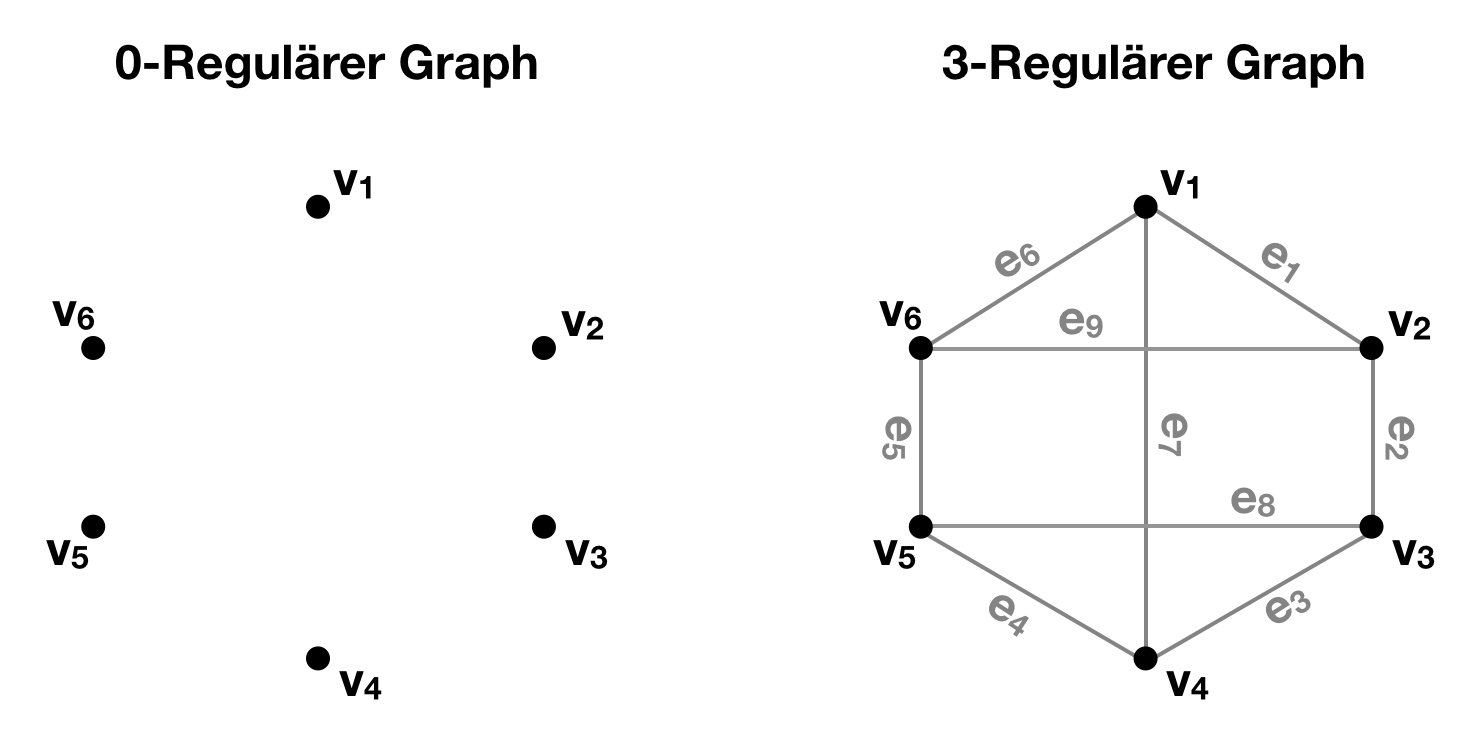
\includegraphics[scale = 0.4]{./images/Regulaerer_graph.png}
%	\label{2.regular.image}
	%\caption{Regulärer Graph}
%\end{center}
Sind bei einem Graphen alle Knoten mit allen übrigen Knoten verbunden, spricht man von einem vollständigen Graphen:
\[K_{n}=\big([n],\begin{pmatrix}
					 [n] \\ 2
\end{pmatrix}\big)\]

%Werden Kanten und Knoten eines Graphs vertauscht, entsteht der Kantengraph bzw. Line-Graph des jeweiligen Graphen L(G).
Da bei einem Graphen nur die Struktur definiert ist, also welcher Knoten über welche Kante mit den anderen Knoten verbunden ist, können Graphen auf unterschiedliche Weisen gezeichnet werden und trotzdem gleich sein.
Sind zwei Graphen gleich, bezeichnet man diese als isomorph \cite[Seite 22]{basicgraphtheory}.
%
%Das simpelste Graphdatenbankmodell ist ein einfacher gelabelter Graph.
%
%Subgraphen
%\subsection{Reguläre Graphen}
%Bei regulären Graphen haben alle Knoten den selben Knotengrad.
%Als Knotengrad wird die Anzahl direkter Nachbarn, also alle Knoten die über eine Kante direkt mit dem betrachteten Knoten verbunden sind, bezeichnet.\cite{felsner2012geometric}
%Abbildung \ref{2.regular.image} zeigt einen regulären Graphen mit Knotengrad null und einen mit einem Grad von drei.
%\begin{center}
%	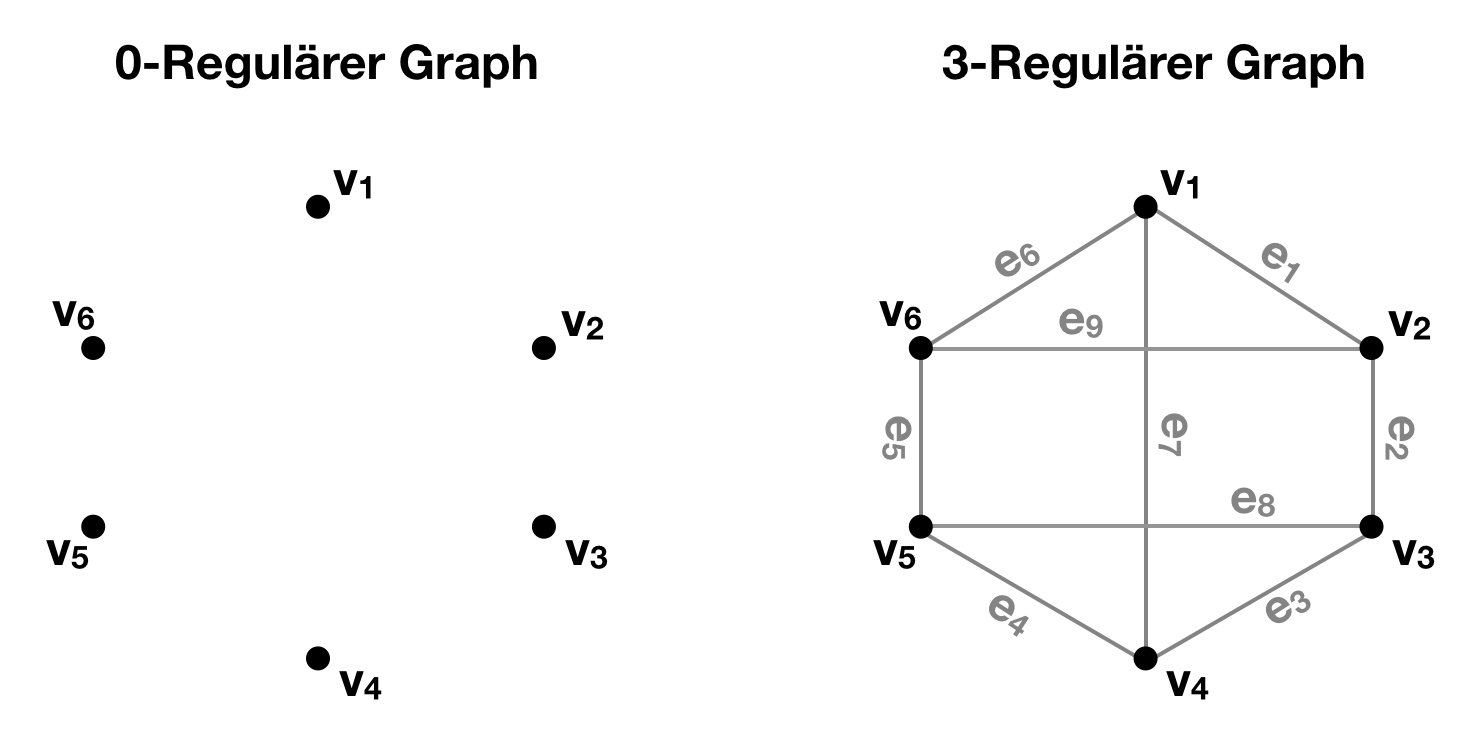
\includegraphics[scale = 0.4]{./images/Regulaerer_graph.png}
%	\label{2.regular.image}
%	%\caption{Regulärer Graph}
%\end{center}
\subsection{Bäume}
Ist ein Graph kreisfrei und es gibt keinen Weg bei dem der Start- gleich dem Endknoten ist, spricht man von einem Wald.
Sind die Knoten eines Waldes zusammenhängend entsteht ein Baum.
%Ein Baum mit $n$ Knoten hat immer $n-1$ Kanten \cite{basicgraphtheory}.
Knoten mit dem Grad $n=1$ werden als Blätter bezeichnet.
Bäume können gerichtet und ungerichtet sein.
Im Falle von gerichteten Bäumen spricht man auch von gewurzelten Bäumen, da der Ursprungsknoten als Wurzel bezeichnet wird.
Abbildung \ref{2.baum.image} zeigt einen gewurzelten Baum, die Blätter sind hier grün dargestellt und die Wurzel rot.
In einem Baum gibt es zwischen zwei beliebigen Knoten immer nur einen Weg \cite{basicgraphtheory}.
%Bei einem gewurzelten Baum werden die Ausgangsknoten als Eltern und die Zielknoten jeweils als Kinder der Ausgangsknoten bezeichnet.
%Hat in einem gewurzelten Baum jeder Knoten maximal zwei Kinder, wird dieser als Binärbaum bezeichnet \cite{basicgraphtheory}.
\begin{figure}[H]
	\begin{center}
	\includegraphics[scale = 0.3]{./images/{2.baum}.png}
	\label{2.baum.image}
    \caption{gewurzelter Baum}
	\end{center}
\end{figure}
Bäume sind Grundlage unteranderen des hierarchischen Datenbankmodells, welches sich dadurch auszeichnet, dass jeder Knoten nur einen Vorgänger haben kann.
Dieses Datenbankmodell hat den Nachteil, dass bedingt durch die Kreisfreiheit eines Baumes sehr eingeschränkt ist und beispielsweise keine n:n Beziehungen modelliert werden können.
Das Netzwerkdatenbankmodell versucht dieses Problem zu lösen, indem die Limitierung auf einen Vorfahren aufgehoben wird \cite{hald2013datenbank}.
\subsection{Property Graphen}
Property Graphen erweitern das Modell des einfachen Graphen.
Property Graphen sind gerichtete Graphen, die sich durch ihre den Kanten und Knoten zugewiesenen Eigenschaften (Properties) auszeichnen.
Gespeichert werden diese Eigenschaften als Key-Value-Paare.
Das Hinzufügen von Attributen an einen Knoten oder eine Kante soll zusammengehörige Daten schneller abrufbar machen \cite{angles2012comparison}.
Label ermöglichen die Unterteilung von Knoten und Kanten in verschiedene Knoten- und Kantentypen.
Attribute, Label und die Richtung der Kanten erlauben eine sehr detaillierte Modellierung von realen Sachverhalten.
Somit sind Property Graphen von sehr großer Bedeutung für die Modellierung von Graphdatenbanken.

Abbildung \ref{2.property.image} zeigt einen Property Graphen.
Die Knoten sind den drei Labeln Person, Unternehmen und Stadt zugeordnet.
Die gerichteten Kanten stellen die Beziehungsverhältnisse zwischen den einzelnen Knoten her und können durch Attribute, wie beispielsweise der Information über die Dauer der bisherigen Beziehung, genauer definiert werden.
\begin{figure}[H]
\begin{center}
	\includegraphics[scale = 0.65]{./images/{2.Property_graph}.png}
	\label{2.property.image}
	\caption{Property Graph}
\end{center}
\end{figure}


Der Vorteil von Property Graphen ist, dass diese eine sehr detailierte Modellierung der Daten ermöglichen.
Nachteilig ist, dass eine komplexere Datenstruktur zu einer komplizierteren Realisierung führt.
Derzeit sind Property Graphen das am häufigsten verwendete Datenmodell für Graphdatenbanken.
Neo4j, die momentan weltweit populärste Graphdatenbank, nutzt Property Graphen als Datenbankmodell \cite{neo4j}.
Ein weiteres Beispiel für ein Graph \ac{DBMS}, welches Property Graphen zur Modellierung nutzt, ist JanusGraph \cite{janus}.

\subsection{Property Graphen}
Property Graphen erweitern das Modell des einfachen Graphen.
Property Graphen sind gerichtete Graphen, die sich durch ihre den Kanten und Knoten zugewiesenen Eigenschaften (Properties) auszeichnen.
Gespeichert werden diese Eigenschaften als Key-Value-Paare.
Das Hinzufügen von Attributen an einen Knoten oder eine Kante soll zusammengehörige Daten schneller abrufbar machen \cite{angles2012comparison}.
Label ermöglichen die Unterteilung von Knoten und Kanten in verschiedene Knoten- und Kantentypen.
Attribute, Label und die Richtung der Kanten erlauben eine sehr detaillierte Modellierung von realen Sachverhalten.
Somit sind Property Graphen von sehr großer Bedeutung für die Modellierung von Graphdatenbanken.

Abbildung \ref{2.property.image} zeigt einen Property Graphen.
Die Knoten sind den drei Labeln Person, Unternehmen und Stadt zugeordnet.
Die gerichteten Kanten stellen die Beziehungsverhältnisse zwischen den einzelnen Knoten her und können durch Attribute, wie beispielsweise der Information über die Dauer der bisherigen Beziehung, genauer definiert werden.
\begin{figure}[H]
\begin{center}
	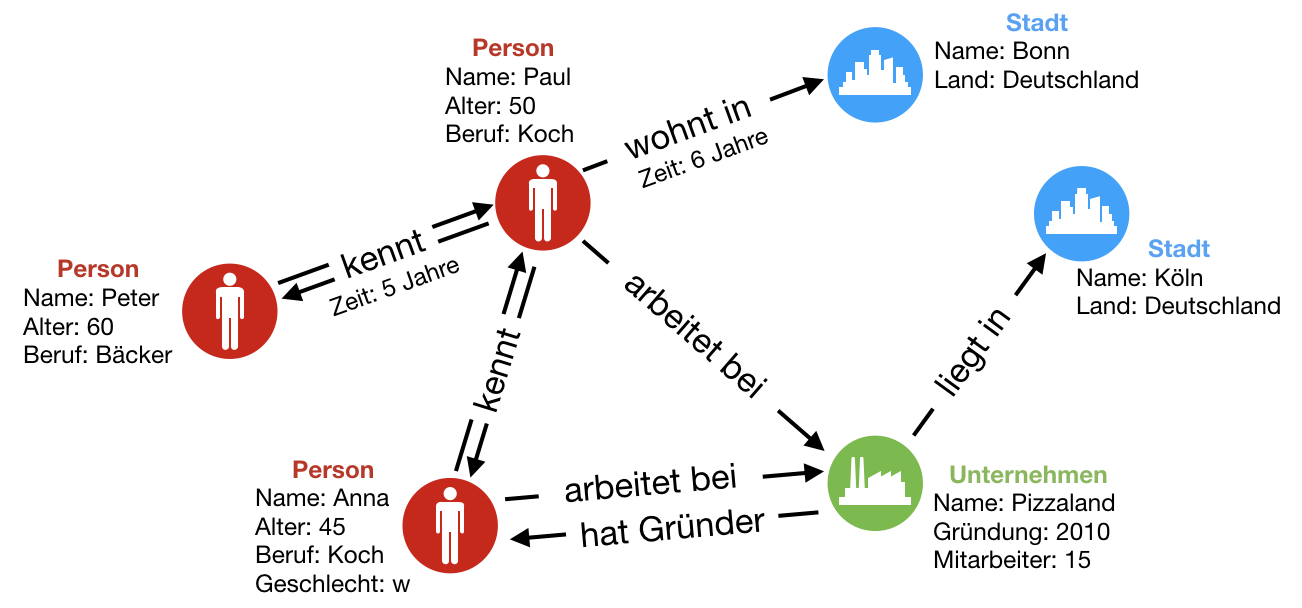
\includegraphics[scale = 0.65]{./images/Property_graph.png}
	\label{2.property.image}
	\caption{Property Graph}
\end{center}
\end{figure}


Der Vorteil von Property Graphen ist, dass diese eine sehr detailierte Modellierung der Daten ermöglichen.
Nachteilig ist, dass eine komplexere Datenstruktur zu einer komplizierteren Realisierung führt.
Derzeit sind Property Graphen das am häufigsten verwendete Datenmodell für Graphdatenbanken.
Neo4j, die momentan weltweit populärste Graphdatenbank, nutzt Property Graphen als Datenbankmodell \cite{neo4j}.
Ein weiteres Beispiel für ein Graph \ac{DBMS}, welches Property Graphen zur Modellierung nutzt, ist JanusGraph \cite{janus}.
\subsection{Hypergraphen}
Hypergraphen stellen eine Generalisierung von Graphen dar und ermöglichen die Modelierung komplexer Beziehungen \cite{anglesintro}.
%Hypergraphen haben die Eigenschaft, dass Kanten im Gegensatz zu klassischen Graphen mehr als zwei Knoten miteinander verbinden können.
%Die Kanten des Hypergraphen werden auch als Hyperkanten bezeichnet.
Im Vergleich zum normalen Graphen können die Kanten eines Hypergraphen eine beliebige Kardinalität haben.
Die Hyperedges in einem Hypergraphen verbinden somit eine beliebige Menge von Knoten, was eine direkte Darstellung von Beziehungen höherer Ordnung ermöglicht \cite{iordanov2010hypergraphdb}.
Im Falle eines gerichteten Hypergraphen verbindet die Hyperkante den Ausgangsknoten direkt mit allen Zielknoten.
%\\Mathematisch ist ein Hypergraph folgendermaßen definiert:
%\begin{definition}
%	Let $X=\{v_{1}, v_{2},...,v_{n}\}$ be a finite set,
%	and let $E=\{e_{1},e_{2},...,e_{m}\}$ be a family of subsets of $X$ such that
%	\[e_{i} \neq \varnothing (i=1,2,...,m) \\
%	\cup_{i=1}^{m}e_{i}=X.
%	\]
%	The pair $H=(X,E)$ is called a hypergraph with vertex set $X$
%	and hyperedge set $E$. The elements $v_{1}, v_{2},...,v_{n}$ of $X$ are vertices
%	of hypergraph $H$, and the sets $e_{1}, e_{2},...,e_{m}$ are hyperedges of hypergraph $H$ \cite[Seite 2]{zhang2018hypergraph}.
%\end{definition}

Abbildung \ref{2.hyper.image} zeigt einen Hypergraphen.
Die Kante $e_{4}$ verbindet in diesem Graphen die Knoten $v_{5}$, $v_{6}$ und $v_{7}$ miteinander.
\begin{figure}[H]
\begin{center}
	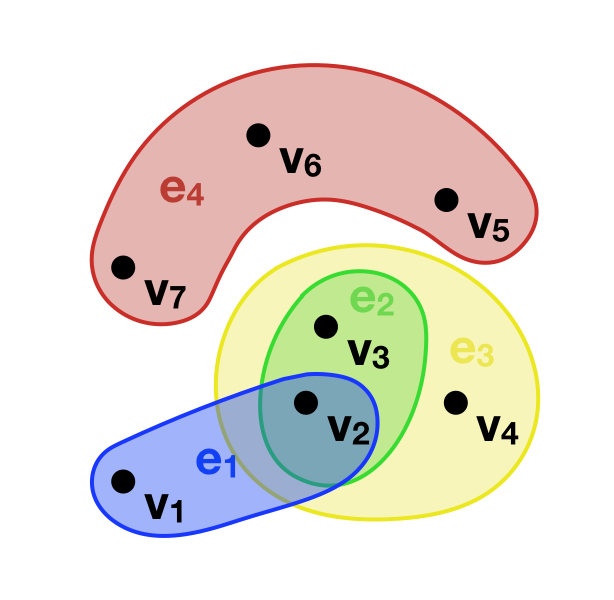
\includegraphics[scale = 0.5]{./images/Hypergraph2.png}
	\label{2.hyper.image}
	\caption{Hypergraph}
\end{center}
\end{figure}
%Hypergraphen ermöglichen die direkte Darstellung rekursiver Beziehungen \cite{iordanov2010hypergraphdb}.
Da Hypergraphen die direkte Darstellung rekursiver Beziehungen ermöglichen und somit eine flexiblere Struktur als das einfache Graphen-Modell bieten, werden diese oft zur Modellierung in Graphdatenbanken verwendet \cite{iordanov2010hypergraphdb}\cite{flockdb}.
Eine Datenbank, die Hypergraphen als Datenbankmodell nutzt ist beispielsweise HyperGraphDB, welche von Kobrix Software Inc entwickelt wurde \cite{iordanov2010hypergraphdb}.
Ein weiteres Projekt, bei dem Hypergraphen zur Modellierung genutzt werden ist Trinity \cite{shao2013trinity}.
%In einem normale Graphen sind die Kanten, eine in einem Intervall festgelegte Menge von Knoten:
%    \[X = \{v_{1}, v_{2}, v_{3}, v_{4}, v_{5}, v_{6}, v_{7}\} \text{ Knoten}\]
%    \[E=\{e_{1}, e_{2}, e_{3}, e_{4}\} \text{ Kanten}\]
%    \[E=\{e_{1}, e_{2}, e_{3}, e_{4}\} = \{\{v_{1}, v_{2}, v_{3}\}, \{v_{2}, v_{3}\}, \{v_{3}, v_{5}, v_{6}\}, \{v_{4}\}\} \]
%Transversals
%\subsection{Multimodale Graphen}
%\subsection{Hypertree}
%\subsection{k-uniform hypergraph}

%\input{2.2}
%\input{3.2}
\chapter{Graph-Datenbanken im praktischen Einsatz: OLAP}
\chapter{Graph-Datenbanken im praktischen Einsatz: OLAP}
\section{PostgreSQL}
Im folgenden Abschnitt werden die in Kapitel 3 vorgestellten SQLs auf ihre Leistungsfähigkeit untersucht. Für die Messung wurden vier verschiedene Stored Procedures angelegt:
\begin{itemize}
	\item innerJoinGenerator
	\item recursivesearch
	\item selectCascadingGenerator
	\item selectUnionGenerator
\end{itemize}
Der Aufruf der Statements funktioniert gleich, es werden die Rekursionstiefe, der Startknoten und die Tabelle, auf welcher die Stored Procedure ausgeführt wird, übergeben.

Die Funktionen innerJoinGenerator, selectCascadingGenerator und selectWithUnionSourceCodeGenerator generieren die entsprechenden Statements und führen diese aus. Die Funktion innerJoinGenerator erzeugt ein Select Statement in der die Abfrage, wie in Abschnitt \ref{2.postgresInnerJoin.subsection} beschrieben, erzeugt und ausgeführt wird. Entsprechend erzeugt selectCascadingGenerator eine verschachtelte Select-Abfrage. Die Funktion ist in Listing \ref{2.StandardSQLGenerisch.listing} abgebildet. Die Funktion selectUnionGenerator erzeugt eine Abfrage wie in Abschnitt \ref{2.postgresStandardSQL.subsection} beschrieben. Bei der Funktion recursivesearch handelt es sich um die Funktion wie sie in Abschnitt \ref{2.postgresRecursiveFunction.subsection} beschrieben.

\subsection{Indexe und Partionierte Tabellen}
Um eine bessere Aussage über die Performance von PostgreSQL zu bekommen wurden zusätzlich zu den ''Default'' --Relationstabellen für jeden Datensatz zwei weitere Tabellen angelegt.

Die erste Tabelle hat das Suffix ''\_with\_index''. Im Listing ist Beispielhaft das Create-Skript für die Relationen aus dem Datensatz ''youtube'' dargestellt:

\lstsetsql
\begin{lstlisting}[language=SQL,caption = Tabelle mit Index anlegen,frame=single, label={2.tabelleIndex.listing} ]
CREATE TABLE IF NOT EXISTS relation_youtube_with_index(
src INTEGER REFERENCES profiles_youtube(ID),
dst INTEGER REFERENCES profiles_youtube(ID),
type VARCHAR(50),
date DATE
);
CREATE INDEX yt_dst ON relation_youtube_with_index (dst);
CREATE INDEX yt_src ON relation_youtube_with_index (src);
\end{lstlisting}

Im Unterschied zur ''public\_youtube''--Tabelle wurde diese Tabelle noch um Zwei Indices erweitert. Dabei wurde ein index auf die src-Spalte angelegt, der andere auf die dst-Spalte.


Neben der den ''\_with\_index''--Tabellen wurden noch die \_partitioned--Tabellen angelegt. Diese verwenden die gleichen Indices wie die ''\_with\_index''-Tabellen, jedoch sind sie zusätzlich in 4 Partitonen aufgteilt:

\begin{lstlisting}[language=SQL,caption = Partitonierte Tabelle mit Indices anlegen,frame=single, label={2.tabelleIndex.listing} ]

CREATE TABLE IF NOT EXISTS relation_youtube_partitioned(
src INTEGER REFERENCES profiles_youtube(ID),
dst INTEGER REFERENCES profiles_youtube(ID),
type VARCHAR(50),
date DATE
)PARTITION BY RANGE(src);
CREATE INDEX yt_part_src ON relation_youtube_partitioned (src);
CREATE INDEX yt_part_dst ON relation_youtube_partitioned (dst);
CREATE TABLE relation_youtube_partitioned_0 PARTITION OF relation_youtube_partitioned
FOR VALUES FROM (0) TO (800000);
CREATE TABLE relation_youtube_partitioned_1 PARTITION OF relation_youtube_partitioned
FOR VALUES FROM (800001) TO (1600000);
CREATE TABLE relation_youtube_partitioned_2 PARTITION OF relation_youtube_partitioned
FOR VALUES FROM (1600001) TO (2400000);
CREATE TABLE relation_youtube_partitioned_3 PARTITION OF relation_youtube_partitioned
FOR VALUES FROM (2400001) TO (3200000);
\end{lstlisting}

Da die Datensätze unterschiedlich groß sind wurden die Partionsgrößen entsprechend angepasst. Jeder Datensatz wurde auf 4 Partitonen verteilt. Damit ergibt sich für den Datensatz youtube eine Partitonsgröße von 800.000.



\subsection{Benchmark}
Mit der Standardinstallation von PostgreSQL wird auch pgbench mitinstalliert. Bei pgbench handelt es sich um ein einfaches Tool zur Durchführung von Benchmark-Tests. Bei einem Benchmark-Test wird eine Menge von \ac{SQL}-Statements beliebig oft wiederholt, dabei können auch mehrere parallele Sessions geöffnet werden. Beim durchführen des Tests berechnet pgbench die durchschnittliche Latenz aller Requests, sowie die Transaktionen pro Sekunde \cite{postgres2018}.
\subsubsection{Verwendung von pgbench}
pgbench wird über die Kommandozeile gestartet. Dabei können eine Reihe von Parametern übergeben werden, mit denen das Verhalten von pgbench gesteuert werden kann.
\begin{itemize}
	\item -c clients  \\
	Über das Flag -c wird die Anzahl der Clients bzw. die Anzahl der gleichzeitigen Datenbankverbindungen festgelegt. Wenn hier nichts angegeben ist wird nur ein Client verewendet.
	\item -t transactions \\
	Über das Flag -t wird festgelegt wieviele Transaktionen jeder Client durchführt. Die Anzahl aller Transaktionen ergibt sich durch das Produkt von Clients und Transactions.
	\item -h hostname \\
	Der Hostname des Datenbankservers.
	\item -p Port \\
	Der Port auf dem die Datenbank hört.
	\item -U login \\
	Der Nutzername mit dem sich pgbench anmeldet. Hier kann kein Passwort angegeben werden. Das Datenbankpasswort kann in die Systemvariable PGPASSWORD geschrieben werden. Diese Varibale wird von pgbench dann ausgwewertet.
	\item -d Database \\
	Die Datenbank gegen die sich pgbench verbindet
	\item -f File \\ 
	Über -f kann jeweils eine Datei mit mehreren SQL-Statements übergeben werden. Eine Transaktion entspricht dabei der Abarbeitung aller SQL-Befehle innerhalb der Datei.
	Wird keine Datei angegeben führt pgbench ein Default-Benchmarking aus.

\end{itemize}
Für die Benchmarktests wurden zehn Clients parallel gestartet werden, die jeweils fünf Transaktionen durchführen sollten. Aus dem Mittelwert dieser 50 Transaktionen wurden bestimmt pgbench Latenz und Transaktionen pro Sekunde.

\begin{lstlisting}[language=bash,caption = pgbench Statment,frame=single, label={2.pgbench.listing} ]
/usr/lib/postgresql/11/bin/pgbench \ 
-h 10.20.110.43 -p 5413 \ 
-U postgres -d team22 \ 
-c 10 -t 5 -f Select_innerjoinsourcecodegenerator_1.sql
\end{lstlisting}
Pgbench kann kein Passwort übergeben werden. Als Workaround kann das Passwort in die Umgebungsvariable PGPASSWORD gespeichert werden. Die Variable wird dann von pgbench ausgewertet. 
\subsubsection{Testaufbau}
Für die Benchmarktests wurde auf dem Master-Node der Ordner pgbench angelegt. Im Ordner pgbench sind eine Reihe von Unterordnern angelegt sowie das Skript pgbench.sh. Dieses Skript erzeugt das pgbench-Statment. Anschließend ruft das Skript sequentiell alle pgbensh.sh-Skripte auf die sich in den Unterordnern befinden auf.
\begin{figure}[H]
\tikzstyle{every node}=[draw=black,thick,anchor=west]
\usetikzlibrary{trees}
\tikzstyle{file}=[draw=none]
\begin{tikzpicture}[%
grow via three points={one child at (0.5,-0.8) and
	two children at (0.5,-0.8) and (0.5,-1.6)},
edge from parent path={(\tikzparentnode.south) |- (\tikzchildnode.west)}]
\node {pgbench}
child{ node[file]{pgbench.sh}}
child { node {public\_epinions}
	child{ node[file]{pgbench.sh}}
	child{node[file]{Select\_innerJoinGenerator\_1.sql}}
	child{node[file]{...}}
}
child [missing] {}
child [missing] {}
child [missing] {}		
child { node {public\_epinions\_with\_index}
child{ node[file]{pgbench.sh}}
child{node[file]{Select\_innerJoinGenerator\_1.sql}}
child{node[file]{...}}
}
child [missing] {}
child [missing] {}
child [missing] {}	
child { node {public\_epinions\_partitioned}
child{ node[file]{pgbench.sh}}
child{node[file]{Select\_innerJoinGenerator\_1.sql}}
child{node[file]{...}}
};
\end{tikzpicture}
%Reset Configuration
\tikzstyle{every node}=[]
\caption{Ordnerstruktur Benchmarktest}
\label{2.pgbenchFile.image}
\end{figure}
Jedes pgbench.sh-Skript startet sequenziell einen pgbench-Benchmarktest mit jeder SQL-Datei im selben Ordner. Jeder Ordner steht dabei für eine der relations-Tabellen. Für jede Kombination aus Rekursionstiefe und SQL-Statement gibt es eine SQL-Datei, welche genau ein Statement enthält.

Nach jedem Durchlauf von pgbench wird folgende Ausgabe erzeugt:

\begin{lstlisting}[caption= Ausgabe pgbench, label={2.outputpgbench.listing}]
pghost: 10.20.110.43 pgport: 5413 nclients: 10 nxacts: 5 dbName: team22
transaction type: Select_innerjoinsourcecodegenerator_1.sql
scaling factor: 1
query mode: simple
number of clients: 10
number of threads: 1
number of transactions per client: 5
number of transactions actually processed: 50/50
latency average = 9.899 ms
tps = 1010.157069 (including connections establishing)
tps = 1104.908743 (excluding connections establishing)
\end{lstlisting}

Der Output von pgbench wird mit Hilfe der pgbench.sh Skripte in eine Logdatei geschrieben. Die Logdatei wird innerhalb jedes Ordners unterhalb von pgbench angelegt.
Für jeden Testlauf wird eine neue Logdatei angelegt. Damit die Logdateien nicht überschrieben werden, wird die Logdatei mit einem Zeitstempel angelegt. So steht zum Beispiel in der Datei unter dem Pfad
 \texttt{/pgbench/public\_epinions\_with\_index /pgbench\_2019\_01\_12\_15\_26.log} die Ausgabe des Benchmarktests für die Tabelle \texttt{public\_epionions\_with\_index} vom 12.1.2019.
 
 In den folgenden drei Abschnitten sind die durchschnittlichen Latenzen aller Tabellen dargestellt. Die Unterteilung erfolgt hierbei nach Tabellen ohne Indices, Tabellen mit Incides und  Partionierte Tabellen mit Indices. 

\newpage
\subsubsection{Antwortzeiten ohne Indices}
In diesem Abschnitt sind die Laufzeiten der verschiedenen SQLs auf den Tabellen ohne Indices dargestellt.
\paragraph{relation\_epinions}\mbox{}\\
\begin{figure}[H]
\begin{tikzpicture}[y=.5cm, x=2cm,font=\sffamily]
%axis
\draw (0,0) -- coordinate (x axis mid) (5,0);
\draw (0,0) -- coordinate (y axis mid) (0,18);
    	%ticks
\foreach \x in {0,...,5}
\draw (\x,1pt) -- (\x,-3pt)
node[anchor=north] {\x};
	\foreach \y/\ytext in {
	0/0,
	1/5000,
	2/10000,
	3/15000,
	4/20000,
	5/25000,
	6/30000,
	7/35000,
	8/40000,
	9/45000,
	10/50000,
	11/55000,
	12/60000,
	13/65000,
	14/70000,
	15/75000,
	16/80000,
	17/85000,
	18/90000
}
\draw (1pt,\y) -- (-3pt,\y) node[anchor=east] {$\ytext$}; 
%labels      
\node[below=0.8cm] at (x axis mid) {Rekursionstiefe};
\node[rotate=90, above=1.5cm] at (y axis mid) {Laufzeit in ms};
%plots
\draw[darkgray] plot[ mark=*, mark options={fill=white}] 
coordinates{(0, 0)
	(1, 61.065/5000)
	(2,231.850/5000)
	(3,333.011/5000)
	(4,3.5545)%17772.456/5000)
	(5,16.2483)%81241.284/5000
};

\draw[red] plot[ mark=*, mark options={fill=white}] 
coordinates{(0, 0)
			(1, 63.636/5000)
			(2,139.225/5000)
			(3,229.997/5000)
			(4,432.297/5000)
			(5,677.420/5000)
		};
\draw[blue] plot[ mark=*, mark options={fill=white}] 
coordinates{(0, 0)
	(1, 89.858/5000)
	(2,168.822/5000)
	(3,273.452/5000)
	(4,513.038/5000)
	(5,921.228/5000)
};
\draw[green] plot[ mark=*, mark options={fill=white}] 
coordinates{(0, 0)
	(1, 59.275/5000)
	(2,143.367/5000)
	(3,277.766/5000)
	(4,1664.168/5000)
	(5,8335.513/5000)
};
\draw (0,-3) -- (5,-3) 
(0,-3) -- (0,-6)
(0,-6) -- (5,-6)
(5,-3) -- (5,-6);
\draw[draw=none] (0,0) -- (5,0) 
node[draw=none, midway, yshift=-4.5em]
{
	\textcolor{darkgray}{--- selectWithInnerJoin}
	\textcolor{green}{--- selectUnionGenerator} 
	
};
\draw[draw=none] (0,-3) -- (5,0) 
node[draw=none, midway, yshift=-4.5em]
{
	\textcolor{blue}{--- recursiveSearch} 
	\textcolor{red}{--- selectCascadingGenerator}
};
\end{tikzpicture}
	\caption{ relation\_epinions}
	\label{2.relationepinions.image}
\end{figure}

% Please add the following required packages to your document preamble:
% \usepackage{multirow}
\begin{table}[H]
	\begin{tabular}{l|l|l|l|l|l|}
		\cline{2-6}
		& \multicolumn{5}{|l|}{Laufzeit in MS}                                                                                                                                                  \\ \hline
		\multicolumn{1}{|l|}{\multirow{2}{2cm}{Rerkusions-tiefe}} & \multicolumn{2}{|l|}{\multirow{2}{3cm}{selectCascading Generator}} & \multirow{2}{2.8cm}{recursiveSearch} & \multirow{2}{2.5cm}{selectUnion Generator} & \multirow{2}{2.5cm}{selectInner JoinGenerator} \\
		\multicolumn{1}{|l|}{}
		& \multicolumn{2}{|l|}{}                                           &                                  &                                     &                                           \\ \hline
	\multicolumn{1}{|l|}{1}               & \multicolumn{2}{l|}{63.636}                                     & 89.858                           & 59.275                              & 61.065                                    \\ \hline
	\multicolumn{1}{|l|}{2}               & \multicolumn{2}{l|}{139.225}                                    & 168.822                          & 143.367                             & 231.850                                   \\ \hline
	\multicolumn{1}{|l|}{3}               & \multicolumn{2}{l|}{229.997}                                    & 273.452                          & 277.766                             & 333.011                                   \\ \hline
	\multicolumn{1}{|l|}{4}               & \multicolumn{2}{l|}{432.297}                                    & 513.038                          & 1664.168                            & 17772.456                                 \\ \hline
	\multicolumn{1}{|l|}{5}               & \multicolumn{2}{l|}{677.420}                                    & 921.228                          & 8335.513                            & 81241.284                                 \\ \hline
	
	\end{tabular}
	\caption{Laufzeit der SQLs für Tabelle relation\_epions}
	\label{2.relationepinions.table}
\end{table}

Bei der relation\_epinions Tabelle zeigen sich ab der 3. Rekursionstufe deutliche Unterschiede in den Laufzeiten der einzelnen Statements. In der Rekursionsstufe 5 schneidet das Innerjoin-Statement mit 81 Sekunden am schlechtesten ab. Das verschachtelte Select ist mit 677 Millisekunden am schnellsten und benötigt dabei nur 
0.8\% der Laufzeit des Innerjoin Statements.

\paragraph{relation\_livejournal}\mbox{}\\

\begin{figure}[H]

	\begin{tikzpicture}[y=.25cm, x=2cm,font=\sffamily]
	%axis
	\draw (0,0) -- coordinate (x axis mid) (5,0);
	\draw (0,0) -- coordinate (y axis mid) (0,24);
	%ticks
	\foreach \x in {0,...,5}
	\draw (\x,1pt) -- (\x,-3pt)
	node[anchor=north] {\x};
	\foreach \y/\ytext in {
		0/0,	
		2/10000,
		4/20000,
		6/30000,
		8/40000,
		10/50000,
		12/60000,
		14/70000,
		16/80000,
		18/90000,
		20/100000,
		22/110000,
		24/120000
	}
	\draw (1pt,\y) -- (-3pt,\y) node[anchor=east] {$\ytext$};
	%labels      
	\node[below=0.8cm] at (x axis mid) {Rekursionstiefe};
	\node[rotate=90, above=1.5cm] at (y axis mid) {Laufzeit in ms};
	%plots
	\draw[darkgray] plot[mark=*, mark options={fill=white}] 
	coordinates{(0, 0)
		(1, 0.9819)%4909.862/5000)
		(2,	4.8836)%24417.787/5000)
		(3, 6.3127)%31563.339/5000)
		(4, 7.5570)%37785.200/5000)
		(5,	11.3202)%56601.185/5000)
	};
	\draw[red] plot[mark=*, mark options={fill=white}] 
	coordinates{(0, 0)
		(1, 4761.733/5000)
		(2,	11589.219/5000)
		(3, 4.9944)	%=24971/5000
		(4, 8.9252) %=44625,935÷5000
		(5,	13.1265944)%=65632,972÷5000
	};
\draw[blue] plot[mark=*, mark options={fill=white}] 
coordinates{(0, 0)
	(1, 1.4151)%7075.399/5000)
	(2,	2.7405)%13702.381/5000)
	(3, 4.1548)%20773.827/5000)
	(4, 5.6098)%28048.866/5000)
	(5,	10.7651)%53825.401/5000)
};
\draw[green] plot[mark=*, mark options={fill=white}] 
coordinates{(0, 0)
	(1, 0.939)%4695.466/5000)
	(2,	8.323)%41616.216/5000)
	(3, 12.916)%64577.873/5000)
	(4, 17.487)%87434.075/5000)	
	(5,	23.086)%115432.071/5000)	
};
	\draw (0,-6) -- (5,-6) 
(0,-6) -- (0,-12)
(0,-12) -- (5,-12)
(5,-6) -- (5,-12);
\draw[draw=none] (0,0) -- (5,0) 
node[draw=none, midway, yshift=-4.5em]
{
	\textcolor{darkgray}{--- selectWithInnerJoin}
	\textcolor{green}{--- selectUnionGenerator} 
	
};
\draw[draw=none] (0,-6) -- (5,0) 
node[draw=none, midway, yshift=-4.5em]
{
	\textcolor{blue}{--- recursiveSearch} 
	\textcolor{red}{--- selectCascadingGenerator}
};
	\end{tikzpicture}
	\caption{ relation\_livejournal}
	\label{2.relationlivejournal.image}
\end{figure}
\begin{table}[H]
	\begin{tabular}{l|l|l|l|l|l|}
		\cline{2-6}
		& \multicolumn{5}{|l|}{Laufzeit in MS}                                                                                                                                                  \\ \hline
		\multicolumn{1}{|l|}{\multirow{2}{2cm}{Rerkusions-tiefe}} & \multicolumn{2}{|l|}{\multirow{2}{3cm}{selectCascading Generator}} & \multirow{2}{2.8cm}{recursiveSearch} & \multirow{2}{2.5cm}{selectUnion Generator} & \multirow{2}{2.5cm}{selectInner JoinGenerator} \\
		\multicolumn{1}{|l|}{}
		& \multicolumn{2}{|l|}{}                                           &                                  &                                     &                                           \\ \hline
		\multicolumn{1}{|l|}{1}                                 & \multicolumn{2}{l|}{4761.733}                                    & 7075.399                                              & 4695.466                                                  & 4909.862                                                        \\ \hline
		\multicolumn{1}{|l|}{2}                                 & \multicolumn{2}{l|}{11589.219}                                   & 13702.381                                             & 41616.216                                                 & 24417.787                                                       \\ \hline
		\multicolumn{1}{|l|}{3}                                 & \multicolumn{2}{l|}{24971}                                       & 20773.831                                             & 64577.873                                                 & 31563.339                                                       \\ \hline
		\multicolumn{1}{|l|}{4}                                 & \multicolumn{2}{l|}{44625.935}                                   & 28048.866                                             & 87434.075                                                 & 37785.200                                                       \\ \hline
		\multicolumn{1}{|l|}{5}                                 & \multicolumn{2}{l|}{65632.972}                                   & 53825.401                                             & 115432.071                                                & 56601.185                                                       \\ \hline
		
	\end{tabular}
	\caption{Laufzeit der SQLs für Tabelle relation\_livejournal}
	\label{2.relationlivejournal.table}
\end{table}

Bei der relation\_livejournal Tabelle sind die Laufzeiten am längsten. Hier schneidet das Standard-SQL am schlechtesten ab. Die Rekursive Stored Procedure ist hier am schnellsten. Jedoch sind die Laufzeiten in der fünften Rekursionsstufe mit im besten Fall 53 Sekunden und im schlechtesten Fall 115 Sekunden sehr lange. Selbst in der ersten Rekursionstufe benötigt eine Abfrage mindestens 4,6 Sekunden.

\paragraph{relation\_facebook}\mbox{}\\

\begin{figure}[H]
	\begin{tikzpicture}[y=.0125cm, x=2cm,font=\sffamily]
	%axis
	\draw (0,0) -- coordinate (x axis mid) (5,0);
	\draw (0,0) -- coordinate (y axis mid) (0,300);
	%ticks
	\foreach \x in {0,...,5}
	\draw (\x,1pt) -- (\x,-3pt)
	node[anchor=north] {\x};
	\foreach \y in {0,50,...,300}
	\draw (1pt,\y) -- (-3pt,\y)
	node[anchor=east] {\y}; 
	%labels      
	\node[below=0.8cm] at (x axis mid) {Rekursionstiefe};
	\node[rotate=90, above=1.5cm] at (y axis mid) {Laufzeit in ms};
	%plots
	\draw[darkgray] plot[ mark=*, mark options={fill=white}] 
	coordinates{(0, 0)
		(1, 10.825)
		(2, 11.119)
		(3, 17.613)
		(4, 61.089)
		(5, 304.821)
	};
	
	\draw[blue] plot[ mark=*, mark options={fill=white}] 
	coordinates{(0, 0)
		(1, 29.595)
		(2,48.442)
		(3,67.989)
		(4,84.084)
		(5,105.049)
	};
	\draw[red] plot[ mark=*, mark options={fill=white}] 
	coordinates{(0, 0)
		(1, 19.528)
		(2,36.613)
		(3,54.681)
		(4,72.934)
		(5,89.262)
	};
	\draw[green] plot[ mark=*, mark options={fill=white}] 
	coordinates{(0, 0)
		(1, 20.716)
		(2,38.137)
		(3,61.904)
		(4,84.295)
		(5,110.000)
	};

	\draw (0,-120) -- (5,-120) 
		  (0,-120) -- (0,-240)
          (0,-240) -- (5,-240)
          (5,-120) -- (5,-240);
\draw[draw=none] (0,0) -- (5,0) 
node[draw=none, midway, yshift=-4.5em]
{
	\textcolor{darkgray}{--- selectWithInnerJoin}
	\textcolor{green}{--- selectUnionGenerator} 
	
};
\draw[draw=none] (0,-120) -- (5,0) 
node[draw=none, midway, yshift=-4.5em]
{
	\textcolor{blue}{--- recursiveSearch} 
	\textcolor{red}{--- selectCascadingGenerator}
};
	\end{tikzpicture}
	\caption{ relation\_facebook}
	\label{2.relationfacebook.image}
\end{figure}

\begin{table}[H]
	\begin{tabular}{l|l|l|l|l|l|}
		\cline{2-6}
		& \multicolumn{5}{|l|}{Laufzeit in MS}                                                                                                                                                  \\ \hline
		\multicolumn{1}{|l|}{\multirow{2}{2cm}{Rerkusions-tiefe}} & \multicolumn{2}{|l|}{\multirow{2}{3cm}{selectCascading Generator}} & \multirow{2}{2.8cm}{recursiveSearch} & \multirow{2}{2.5cm}{selectUnion Generator} & \multirow{2}{2.5cm}{selectInner JoinGenerator} \\
		\multicolumn{1}{|l|}{}
		& \multicolumn{2}{|l|}{}                                           &                                  &                                     &                                           \\ \hline
		\multicolumn{1}{|l|}{1}                                 & \multicolumn{2}{l|}{19.528}                                      & 29.595                                                & 20.716                                                    & 10.825                                                          \\ \hline
		\multicolumn{1}{|l|}{2}                                 & \multicolumn{2}{l|}{36.613}                                      & 48.442                                                & 38.137                                                    & 11.119                                                          \\ \hline
		\multicolumn{1}{|l|}{3}                                 & \multicolumn{2}{l|}{54.681}                                      & 67.989                                                & 61.904                                                    & 17.613                                                          \\ \hline
		\multicolumn{1}{|l|}{4}                                 & \multicolumn{2}{l|}{72.934}                                      & 84.084                                                & 84.295                                                    & 61.089                                                          \\ \hline
		\multicolumn{1}{|l|}{5}                                 & \multicolumn{2}{l|}{89.262}                                      & 105.049                                               & 110.000                                                   & 304.821                                                         \\ \hline
		
		
	\end{tabular}
	\caption{Laufzeit der SQLs für Tabelle relation\_facebook}
	\label{2.relationfacebook.table}
\end{table}

Bei den facebook-Daten ist das Laufzeitverhalten des verschachtelten Selects, der rekursiven Funktion und dem Standard SQL gleich. Die Unterschiede in der Latenz sind im Verhältnis zur Latenz gering. Einen Sonderfall bildet das innerJoin hier ist ab der dritten Rekursionsstufe ein exponentieller Anstieg der Laufzeit zu beobachten. Ab der ersten bis zur einschlieĺich vierten Rekursionstufe ist das innerJoin jedoch am Performantesten.

\newpage

\paragraph{relation\_wiki\_vote}\mbox{}\\

\begin{figure}[H]
	\begin{tikzpicture}[y=.0025cm, x=2cm,font=\sffamily]
	%axis
	\draw (0,0) -- coordinate (x axis mid) (5,0);
	\draw (0,0) -- coordinate (y axis mid) (0,3000);
	%ticks
	\foreach \x in {0,...,5}
	\draw (\x,1pt) -- (\x,-3pt)
	node[anchor=north] {\x};
	\foreach \y in {0,200,...,3000}
	\draw (1pt,\y) -- (-3pt,\y)
	node[anchor=east] {\y}; 
	%labels      
	\node[below=0.8cm] at (x axis mid) {Rekursionstiefe};
	\node[rotate=90, above=1.5cm] at (y axis mid) {Laufzeit in ms};
	%plots
	\draw[darkgray] plot[ mark=*, mark options={fill=white}] 
	coordinates{(0, 0)
		(1, 21.182)
		(2, 62.066)
		(3, 86.128)
		(4, 171.283)
		(5, 2787.659)
	};
	
	\draw[blue] plot[ mark=*, mark options={fill=white}] 
	coordinates{(0, 0)
		(1, 34.365)
		(2, 60.394)
		(3, 80.454)
		(4, 130.866)
		(5, 180.301)
	};
	\draw[red] plot[ mark=*, mark options={fill=white}] 
	coordinates{(0, 0)
		(1, 20.774)
		(2, 40.090)
		(3, 63.405)
		(4, 99.210)
		(5, 144.089)
	};
	\draw[green] plot[ mark=*, mark options={fill=white}] 
	coordinates{(0, 0)
		(1, 21.490)
		(2, 41.234)
		(3, 70.961)
		(4, 215.687)
		(5,1034.360)
	};
	
	\draw (0,-600) -- (5,-600) 
	(0,-600) -- (0,-1200)
	(0,-1200) -- (5,-1200)
	(5,-600) -- (5,-1200);
	\draw[draw=none] (0,0) -- (5,0) 
	node[draw=none, midway, yshift=-4.5em]
	{
		\textcolor{darkgray}{--- selectWithInnerJoin}
		\textcolor{green}{--- selectUnionGenerator} 
		
	};
	\draw[draw=none] (0,-600) -- (5,0) 
	node[draw=none, midway, yshift=-4.5em]
	{
		\textcolor{blue}{--- recursiveSearch} 
		\textcolor{red}{--- selectCascadingGenerator}
	};
	\end{tikzpicture}
	\caption{ relation\_wiki\_vote}
	\label{2.relationwikivote.image}
\end{figure}

\begin{table}[H]
	\begin{tabular}{l|l|l|l|l|l|}
		\cline{2-6}
		& \multicolumn{5}{|l|}{Laufzeit in MS}                                                                                                                                                  \\ \hline
		\multicolumn{1}{|l|}{\multirow{2}{2cm}{Rerkusions-tiefe}} & \multicolumn{2}{|l|}{\multirow{2}{3cm}{selectCascading Generator}} & \multirow{2}{2.8cm}{recursiveSearch} & \multirow{2}{2.5cm}{selectUnion Generator} & \multirow{2}{2.5cm}{selectInner JoinGenerator} \\
		\multicolumn{1}{|l|}{}
		& \multicolumn{2}{|l|}{}                                           &                                  &                                     &                                           \\ \hline
		
		\multicolumn{1}{|l|}{1}                                 & \multicolumn{2}{l|}{20.774}                                      & 34.365                                                & 21.490                                                    & 21.182                                                          \\ \hline
		\multicolumn{1}{|l|}{2}                                 & \multicolumn{2}{l|}{40.090}                                      & 60.394                                                & 41.234                                                    & 62.066                                                          \\ \hline
		\multicolumn{1}{|l|}{3}                                 & \multicolumn{2}{l|}{63.405}                                      & 80.454                                                & 70.961                                                    & 86.128                                                          \\ \hline
		\multicolumn{1}{|l|}{4}                                 & \multicolumn{2}{l|}{99.210}                                      & 130.866                                               & 215.687                                                   & 171.283                                                         \\ \hline
		\multicolumn{1}{|l|}{5}                                 & \multicolumn{2}{l|}{144.089}                                     & 180.301                                               & 1034.360                                                  & 2787.659                                                        \\ \hline
		
		
		
	\end{tabular}
	\caption{Laufzeit der SQLs für Tabelle relation\_wiki\_vote}
	\label{2.relationwikivote.table}
\end{table}

Bei den Wikipedia-Daten zeigt sich ein ähnliches Laufzeitverhalten wie bei den Epionions-Daten. InnerJoin und Standard-SQL verschlechtern sich von der vierten auf die fünfte Iterationsstufe massiv. Das verschachtelte Select weist hier über alle Rekursionsstufen die geringste Latenz auf.

\newpage

\paragraph{relation\_youtube}\mbox{}\\

\begin{figure}[H]
	\begin{tikzpicture}[y=.00125cm, x=2cm,font=\sffamily]
	%axis
	\draw (0,0) -- coordinate (x axis mid) (5,0);
	\draw (0,0) -- coordinate (y axis mid) (0,6000);
	%ticks
	\foreach \x in {0,...,5}
	\draw (\x,1pt) -- (\x,-3pt)
	node[anchor=north] {\x};
	\foreach \y in {0,400,...,6000}
	\draw (1pt,\y) -- (-3pt,\y)
	node[anchor=east] {\y}; 
	%labels      
	\node[below=0.8cm] at (x axis mid) {Rekursionstiefe};
	\node[rotate=90, above=1.5cm] at (y axis mid) {Laufzeit in ms};
	%plots
	\draw[darkgray] plot[ mark=*, mark options={fill=white}] 
	coordinates{(0, 0)
		(1, 421.124)
		(2, 1615.843)
		(3, 2229.214)
		(4, 4082.179)
		(5, 5839.987)
	};
	
	\draw[blue] plot[ mark=*, mark options={fill=white}] 
	coordinates{(0, 0)
		(1, 592.063)
		(2, 1192.278)
		(3, 1793.281)
		(4, 2383.885)
		(5, 2964.950)
	};
	\draw[red] plot[ mark=*, mark options={fill=white}] 
	coordinates{(0, 0)
		(1, 421.464)
		(2, 986.995)
		(3, 1591.391)
		(4, 2250.832)
		(5, 2905.167)
	};
	\draw[green] plot[ mark=*, mark options={fill=white}] 
	coordinates{(0, 0)
		(1, 418.105)
		(2, 1585.836)
		(3, 1654.011)
		(4, 1615.986)
		(5, 1681.231)
	};
	
	\draw (0,-1200) -- (5,-1200) 
	(0,-1200) -- (0,-2400)
	(0,-2400) -- (5,-2400)
	(5,-1200) -- (5,-2400);
	\draw[draw=none] (0,0) -- (5,0) 
	node[draw=none, midway, yshift=-4.5em]
	{
		\textcolor{darkgray}{--- selectWithInnerJoin}
		\textcolor{green}{--- selectUnionGenerator} 
		
	};
	\draw[draw=none] (0,-1200) -- (5,0) 
	node[draw=none, midway, yshift=-4.5em]
	{
		\textcolor{blue}{--- recursiveSearch} 
		\textcolor{red}{--- selectCascadingGenerator}
	};
	\end{tikzpicture}
	\caption{ relation\_youtube}
	\label{2.relationyoutube.image}
\end{figure}

\begin{table}[H]
	\begin{tabular}{l|l|l|l|l|l|}
		\cline{2-6}
		& \multicolumn{5}{|l|}{Laufzeit in MS}                                                                                                                                                  \\ \hline
		\multicolumn{1}{|l|}{\multirow{2}{2cm}{Rerkusions-tiefe}} & \multicolumn{2}{|l|}{\multirow{2}{3cm}{selectCascading Generator}} & \multirow{2}{2.8cm}{recursiveSearch} & \multirow{2}{2.5cm}{selectUnion Generator} & \multirow{2}{2.5cm}{selectInner JoinGenerator} \\
		\multicolumn{1}{|l|}{}
		& \multicolumn{2}{|l|}{}                                           &                                  &                                     &                                           \\ \hline
		
		\multicolumn{1}{|l|}{1}                                 & \multicolumn{2}{l|}{421.464}                                     & 592.063                                               & 418.105                                                   & 421.124                                                         \\ \hline
		\multicolumn{1}{|l|}{2}                                 & \multicolumn{2}{l|}{986.995}                                     & 1192.278                                              & 1585.836                                                  & 1615.843                                                        \\ \hline
		\multicolumn{1}{|l|}{3}                                 & \multicolumn{2}{l|}{1591.391}                                    & 1793.281                                              & 1654.011                                                  & 2229.214                                                        \\ \hline
		\multicolumn{1}{|l|}{4}                                 & \multicolumn{2}{l|}{2250.832}                                    & 2383.885                                              & 1615.986                                                  & 4082.179                                                        \\ \hline
		\multicolumn{1}{|l|}{5}                                 & \multicolumn{2}{l|}{2905.167}                                    & 2964.950                                              & 1681.231                                                  & 5839.987                                                        \\ \hline
		
		
		
	\end{tabular}
	\caption{Laufzeit der SQLs für Tabelle relation\_youtube}
	\label{2.relationyoutube.table}
\end{table}

Bei den Youtube-Daten zeigen die Verschiedenen SQL-Statements ein sehr unterschiedliches Verhalten. Beim Standard-SQL gibt es einen deutlichen Anstieg zwischen von der ersten auf die zweite Rekursionstiefe. Für die weiteren Rekursionstiefen bleibt die Laufzeit dann ungefähr konstant. Das verschachtelte Select und die rekursive Funktion sind in ihrem Laufzeitverhalten sehr ähnlich. Beide steigen linear. Das InnerJoin zweigt bei steigender Rekursionstiefe das schlechteste Laufzeitverhalten.

\subsubsection{Antwortzeiten mit Indices}

Im Folgenden sind die Laufzeiten der SQL-Staments auf den Tabellen mit den Indices dargestellt.

\paragraph{relation\_epinions\_with\_index}\mbox{}\\

\begin{figure}[H]
	\begin{tikzpicture}[y=.5cm, x=2cm,font=\sffamily]
	%axis
	\draw (0,0) -- coordinate (x axis mid) (5,0);
	\draw (0,0) -- coordinate (y axis mid) (0,16);
	%ticks
	\foreach \x in {0,...,5}
	\draw (\x,1pt) -- (\x,-3pt)
	node[anchor=north] {\x};
	\foreach \y/\ytext in {
		0/0,
		1/5000,
		2/10000,
		3/15000,
		4/20000,
		5/25000,
		6/30000,
		7/35000,
		8/40000,
		9/45000,
		10/50000,
		11/55000,
		12/60000,
		13/65000,
		14/70000,
		15/75000,
		16/80000
	}
		\draw (1pt,\y) -- (-3pt,\y) node[anchor=east] {$\ytext$}; 
	%labels      
	\node[below=0.8cm] at (x axis mid) {Rekursionstiefe};
	\node[rotate=90, above=1.5cm] at (y axis mid) {Laufzeit in ms};
	%plots
	\draw[darkgray] plot[ mark=*, mark options={fill=white}] 
	coordinates{(0, 0)
		(1, 10.596/5000)
		(2, 10.739/5000)
		(3, 41.171/5000)
		(4, 0.3696)%1898.726/5000
		(5, 16.2872)%81436.561/5000
	};
	
	\draw[red] plot[ mark=*, mark options={fill=white}] 
	coordinates{(0, 0)
		(1, 8.231/5000)
		(2, 9.290/5000)
		(3, 36.244/5000)
		(4, 235.146/5000)
		(5, 504.793/5000)
	};
	\draw[blue] plot[ mark=*, mark options={fill=white}] 
	coordinates{(0, 0)
		(1, 18.999/5000)
		(2, 23.549/5000)
		(3, 54.953/5000)
		(4, 287.319/5000)
		(5, 737.300/5000)
	};
	\draw[green] plot[ mark=*, mark options={fill=white}] 
	coordinates{(0, 0)
		(1, 8.855/5000)
		(2, 10.304/5000)
		(3, 78.303/5000)
		(4, 2024.069/5000)
		(5, 12920.747/5000)
	};
	\draw (0,-3) -- (5,-3) 
(0,-3) -- (0,-6)
(0,-6) -- (5,-6)
(5,-3) -- (5,-6);
\draw[draw=none] (0,0) -- (5,0) 
node[draw=none, midway, yshift=-4.5em]
{
	\textcolor{darkgray}{--- selectWithInnerJoin}
	\textcolor{green}{--- selectUnionGenerator} 
	
};
\draw[draw=none] (0,-3) -- (5,0) 
node[draw=none, midway, yshift=-4.5em]
{
	\textcolor{blue}{--- recursiveSearch} 
	\textcolor{red}{--- selectCascadingGenerator}
};
	\end{tikzpicture}
	\caption{ relation\_epinions\_with\_index}
	\label{2.relationepinionsindex.image}
\end{figure}

\begin{table}[H]
	\centering
	\begin{tabular}{l|l|l|l|l|l|}
		\cline{2-6}
		& \multicolumn{5}{|l|}{Laufzeit in MS}                                                                                                                                                  \\ \hline
		\multicolumn{1}{|l|}{\multirow{2}{2cm}{Rerkusions-tiefe}} & \multicolumn{2}{|l|}{\multirow{2}{3cm}{selectCascading Generator}} & \multirow{2}{2.8cm}{recursiveSearch} & \multirow{2}{2.5cm}{selectUnion Generator} & \multirow{2}{2.5cm}{selectInner JoinGenerator} \\
		\multicolumn{1}{|l|}{}
		& \multicolumn{2}{|l|}{}                                           &                                  &                                     &                                           \\ \hline
		
		
\multicolumn{1}{|l|}{1}                                 & \multicolumn{2}{l|}{8.231}                                       & 18.999                                                & 8.885                                                     & 10.596                                                          \\ \hline
\multicolumn{1}{|l|}{2}                                 & \multicolumn{2}{l|}{9.290}                                       & 23.549                                                & 10.304                                                    & 10.739                                                          \\ \hline
\multicolumn{1}{|l|}{3}                                 & \multicolumn{2}{l|}{36.244}                                      & 54.953                                                & 78.303                                                    & 41.171                                                          \\ \hline
\multicolumn{1}{|l|}{4}                                 & \multicolumn{2}{l|}{235.146}                                     & 287.319                                               & 2024.069                                                  & 1898.726                                                        \\ \hline
\multicolumn{1}{|l|}{5}                                 & \multicolumn{2}{l|}{504.793}                                     & 737.300                                               & 12920.747                                                 & 81436.561                                                       \\ \hline

	\end{tabular}
	\caption{Laufzeit der SQLs für Tabelle relation\_epinions\_with\_index}
	\label{2.relationepinionsindex.table}
\end{table}

Bei den Epinions-Daten wirkt sich das Einführen der Indices gering aus. Beim innerJoin ist praktisch kein Unterschied zu messbar. Beim StandardSQL führte es sogar zu einer deutlichen Verschlechterung in der fünften Rekursionstufe. Beim verschachtelten Select und bei der rekursieven Funktion gab es eine Verbesserung, diese viel jedoch verhältnismäßig gering aus. Im besten Fall verbesserte sich die fünfte Rekursionstufe von 677 Millisekunden auf 505 Millisekunden.

\paragraph{relation\_livejournal\_with\_index}\mbox{}\\
\begin{figure}[H]
	
	\begin{tikzpicture}[y=.5cm, x=2cm,font=\sffamily]
	%axis
	\draw (0,0) -- coordinate (x axis mid) (5,0);
	\draw (0,0) -- coordinate (y axis mid) (0,16);
	%ticks
	\foreach \x in {0,...,5}
	\draw (\x,1pt) -- (\x,-3pt)
	node[anchor=north] {\x};
	\foreach \y/\ytext in {
		0/0,
		1/2000,
		2/4000,
		3/6000,
		4/8000,
		5/10000,
		6/12000,
		7/14000,
		8/16000,
		9/18000,
		10/20000,
		11/22000,
		12/24000,
		13/26000,
		14/28000,
		15/30000,
		16/32000,
	}
	\draw (1pt,\y) -- (-3pt,\y) node[anchor=east] {$\ytext$};
	%labels      
	\node[below=0.8cm] at (x axis mid) {Rekursionstiefe};
	\node[rotate=90, above=1.5cm] at (y axis mid) {Laufzeit in ms};
	%plots
	
	\draw[darkgray] plot[mark=*, mark options={fill=white}] 
	coordinates{(0, 0)
		(1, 9.165/2000)
		(2,	11.862/2000)
		(3, 8042.794/2000)
		(4, 14865.814/2000)
		(5,	 15.995)%31990.436/2000)
	};	
	\draw[red] plot[mark=*, mark options={fill=white}] 
	coordinates{(0, 0)
		(1, 0.004)%8.672/2000
		(2,	15.240/2000)
		(3, 6936.935/2000)
		(4, 14137.544/2000)%
		(5,	11.232)%22464.363/2000	
	};
	\draw[blue] plot[mark=*, mark options={fill=white}] 
	coordinates{(0, 0)
		(1, 42.010/2000)
		(2,	69.129/2000)
		(3, 114.466/2000)
		(4, 484.914/2000)
		(5,	3830.355/2000)
	};
	\draw[green] plot[mark=*, mark options={fill=white}] 
	coordinates{(0, 0)
		(1, 139.294/2000)
		(2,	131.623/2000)
		(3, 157.707/2000)
		(4, 705.293/2000)
		(5, 6140.824/2000)
	};
	\draw (0,-3) -- (5,-3) 
(0,-3) -- (0,-6)
(0,-6) -- (5,-6)
(5,-3) -- (5,-6);
\draw[draw=none] (0,0) -- (5,0) 
node[draw=none, midway, yshift=-4.5em]
{
	\textcolor{darkgray}{--- selectWithInnerJoin}
	\textcolor{green}{--- selectUnionGenerator} 
	
};
\draw[draw=none] (0,-3) -- (5,0) 
node[draw=none, midway, yshift=-4.5em]
{
	\textcolor{blue}{--- recursiveSearch} 
	\textcolor{red}{--- selectCascadingGenerator}
};
	\end{tikzpicture}
	\caption{ relation\_livejournal\_with\_index}
	\label{2.relationlivejournalindex.image}
\end{figure}

\begin{table}[H]
	\centering
	\begin{tabular}{l|l|l|l|l|l|}
		\cline{2-6}
		& \multicolumn{5}{|l|}{Laufzeit in MS}                                                                                                                                                  \\ \hline
		\multicolumn{1}{|l|}{\multirow{2}{2cm}{Rerkusions-tiefe}} & \multicolumn{2}{|l|}{\multirow{2}{3cm}{selectCascading Generator}} & \multirow{2}{2.8cm}{recursiveSearch} & \multirow{2}{2.5cm}{selectUnion Generator} & \multirow{2}{2.5cm}{selectInner JoinGenerator} \\
		\multicolumn{1}{|l|}{}
		& \multicolumn{2}{|l|}{}                                           &                                  &                                     &                                           \\ \hline
		
		
		\multicolumn{1}{|l|}{1}                                 & \multicolumn{2}{l|}{8.672}                                       & 42.010                                                & 139.294                                                   & 9.165                                                           \\ \hline
		\multicolumn{1}{|l|}{2}                                 & \multicolumn{2}{l|}{15.240}                                      & 69.129                                                & 131.623                                                   & 11.862                                                          \\ \hline
		\multicolumn{1}{|l|}{3}                                 & \multicolumn{2}{l|}{6936.935}                                    & 114.466                                               & 157.707                                                   & 8042.794                                                        \\ \hline
		\multicolumn{1}{|l|}{4}                                 & \multicolumn{2}{l|}{14137.544}                                   & 484.914                                               & 705.293                                                   & 14865.814                                                       \\ \hline
		\multicolumn{1}{|l|}{5}                                 & \multicolumn{2}{l|}{22464.363}                                   & 3830.355                                              & 6140.824                                                  & 31990.436                                                       \\ \hline
	\end{tabular}
	\caption{Laufzeit der SQLs für Tabelle relation\_livejournal\_with\_index}
	\label{2.relationlivejournalindex.table}
\end{table}
Die Verwendung der Indices führt zu einer erheblich besseren Latenz. Die Laufzeit in der ersten Rekursionsstufe verbessert sich von von mindestens 4,7 Sekunden auf im besten Fall 8.7 Millisekunden. Auch in der fünften Rekursionsstufe verkürtzt sich die Laufzeit deutlich.

\paragraph{relation\_facebook\_with\_index}\mbox{}\\

\begin{figure}[H]
	\begin{tikzpicture}[y=.025cm, x=2cm,font=\sffamily]
	%axis
	\draw (0,0) -- coordinate (x axis mid) (5,0);
	\draw (0,0) -- coordinate (y axis mid) (0,300);
	%ticks
	\foreach \x in {0,...,5}
	\draw (\x,1pt) -- (\x,-3pt)
	node[anchor=north] {\x};
	\foreach \y in {0,30,...,300}
	\draw (1pt,\y) -- (-3pt,\y)
	node[anchor=east] {\y}; 
	%labels      
	\node[below=0.8cm] at (x axis mid) {Rekursionstiefe};
	\node[rotate=90, above=1.5cm] at (y axis mid) {Laufzeit in ms};
	%plots
	\draw[darkgray] plot[ mark=*, mark options={fill=white}] 
	coordinates{(0, 0)
		(1, 8.585)
		(2, 9.565)
		(3, 15.738)
		(4, 60.976)
		(5, 297.115)
	};
	
	\draw[blue] plot[ mark=*, mark options={fill=white}] 
	coordinates{(0, 0)
		(1, 20.674)
		(2, 22.639)
		(3, 27.788)
		(4, 32.804)
		(5, 37.706)
	};
	\draw[red] plot[ mark=*, mark options={fill=white}] 
	coordinates{(0, 0)
		(1, 8.594)
		(2, 9.239)
		(3, 26.683)
		(4, 43.610)
		(5, 64.882)
	};
	\draw[green] plot[ mark=*, mark options={fill=white}] 
	coordinates{(0, 0)
		(1, 11.672)
		(2, 11.787)
		(3, 19.625)
		(4, 32.817)
		(5, 48.580)
	};
	
	\draw (0,-60) -- (5,-60) 
	(0,-60) -- (0,-120)
	(0,-120) -- (5,-120)
	(5,-60) -- (5,-120);
	\draw[draw=none] (0,0) -- (5,0) 
	node[draw=none, midway, yshift=-4.5em]
	{
		\textcolor{darkgray}{--- selectWithInnerJoin}
		\textcolor{green}{--- selectUnionGenerator} 
		
	};
	\draw[draw=none] (0,-60) -- (5,0) 
	node[draw=none, midway, yshift=-4.5em]
	{
		\textcolor{blue}{--- recursiveSearch} 
		\textcolor{red}{--- selectCascadingGenerator}
	};
	\end{tikzpicture}
	\caption{ relation\_facebook\_with\_index}
	\label{2.relationfacebookindex.image}
\end{figure}

\begin{table}[H]
	\centering
	\begin{tabular}{l|l|l|l|l|l|}
		\cline{2-6}
		& \multicolumn{5}{|l|}{Laufzeit in MS}                                                                                                                                                  \\ \hline
		\multicolumn{1}{|l|}{\multirow{2}{2cm}{Rerkusions-tiefe}} & \multicolumn{2}{|l|}{\multirow{2}{3cm}{selectCascading Generator}} & \multirow{2}{2.8cm}{recursiveSearch} & \multirow{2}{2.5cm}{selectUnion Generator} & \multirow{2}{2.5cm}{selectInner JoinGenerator} \\
		\multicolumn{1}{|l|}{}
		& \multicolumn{2}{|l|}{}                                           &                                  &                                     &                                           \\ \hline
		
		\multicolumn{1}{|l|}{1}                                 & \multicolumn{2}{l|}{8.594}                                       & 20.674                                                & 11.672                                                    & 8.585                                                           \\ \hline
		\multicolumn{1}{|l|}{2}                                 & \multicolumn{2}{l|}{9.239}                                       & 22.639                                                & 11.787                                                    & 9.565                                                           \\ \hline
		\multicolumn{1}{|l|}{3}                                 & \multicolumn{2}{l|}{26.683}                                      & 27.788                                                & 19.625                                                    & 15.738                                                          \\ \hline
		\multicolumn{1}{|l|}{4}                                 & \multicolumn{2}{l|}{43.610}                                      & 32.804                                                & 32.817                                                    & 60.976                                                              \\ \hline
		\multicolumn{1}{|l|}{5}                                 & \multicolumn{2}{l|}{64.882}                                      & 37.706                                                & 48.580                                                    & 297.115                                                         \\ \hline
	\end{tabular}
	\caption{Laufzeit der SQLs für Tabelle relation\_facebook\_with\_index}
	\label{2.relationfacebookindex.table}
\end{table}

Bei den Facebook Daten lässt sich durch die Indices in fast allen Fällen eine Verbesserung der Latenz erreichen. Außnahme ist hier der InnerJoin, hier ist keine wirkliche Verbesserung erkannbar. In der fünften Rekursionsstufe liegt die Latenz im besten Fall bei 38 Millisekunden mit der rekursiven Funktion. Ohne Indices liegt dieser Wert bei 89 Millisekunden und wird durch das verschachtelte SQL erreicht. 

\paragraph{relation\_wiki\_vote\_with\_index}\mbox{}\\

\begin{figure}[H]
	\begin{tikzpicture}[y=.0025cm, x=2cm,font=\sffamily]
	%axis
	\draw (0,0) -- coordinate (x axis mid) (5,0);
	\draw (0,0) -- coordinate (y axis mid) (0,3000);
	%ticks
	\foreach \x in {0,...,5}
	\draw (\x,1pt) -- (\x,-3pt)
	node[anchor=north] {\x};
	\foreach \y in {0,200,...,3000}
	\draw (1pt,\y) -- (-3pt,\y)
	node[anchor=east] {\y}; 
	%labels      
	\node[below=0.8cm] at (x axis mid) {Rekursionstiefe};
	\node[rotate=90, above=1.5cm] at (y axis mid) {Laufzeit in ms};
	%plots
	\draw[darkgray] plot[ mark=*, mark options={fill=white}] 
	coordinates{(0, 0)
		(1, 8.481)
		(2, 9.903)
		(3, 18.657)
		(4, 130.842)
		(5, 2722.908)
	};
	
	\draw[blue] plot[ mark=*, mark options={fill=white}] 
	coordinates{(0, 0)
		(1, 34.144)
		(2, 54.617)
		(3, 85.721)
		(4, 130.150)
		(5, 183.301)
	};
	\draw[red] plot[ mark=*, mark options={fill=white}] 
	coordinates{(0, 0)
		(1, 8.716)
		(2, 8.868)
		(3, 32.682)
		(4, 68.856)
		(5, 114.462)
	};
	\draw[green] plot[ mark=*, mark options={fill=white}] 
	coordinates{(0, 0)
		(1, 10.474)
		(2, 30.212)
		(3, 58.762)
		(4, 210.655)
		(5, 1031.234)
	};
	
	\draw (0,-600) -- (5,-600) 
	(0,-600) -- (0,-1200)
	(0,-1200) -- (5,-1200)
	(5,-600) -- (5,-1200);
	\draw[draw=none] (0,0) -- (5,0) 
	node[draw=none, midway, yshift=-4.5em]
	{
		\textcolor{darkgray}{--- selectWithInnerJoin}
		\textcolor{green}{--- selectUnionGenerator} 
		
	};
	\draw[draw=none] (0,-600) -- (5,0) 
	node[draw=none, midway, yshift=-4.5em]
	{
		\textcolor{blue}{--- recursiveSearch} 
		\textcolor{red}{--- selectCascadingGenerator}
	};
	\end{tikzpicture}
	\caption{ relation\_wiki\_vote}
	\label{2.relationwikivoteindex.image}
\end{figure}



\begin{table}[H]
	\centering
	\begin{tabular}{l|l|l|l|l|l|}
		\cline{2-6}
		& \multicolumn{5}{|l|}{Laufzeit in MS}                                                                                                                                                  \\ \hline
		\multicolumn{1}{|l|}{\multirow{2}{2cm}{Rerkusions-tiefe}} & \multicolumn{2}{|l|}{\multirow{2}{3cm}{selectCascading Generator}} & \multirow{2}{2.8cm}{recursiveSearch} & \multirow{2}{2.5cm}{selectUnion Generator} & \multirow{2}{2.5cm}{selectInner JoinGenerator} \\
		\multicolumn{1}{|l|}{}
		& \multicolumn{2}{|l|}{}                                           &                                  &                                     &                                           \\ \hline
		
	\multicolumn{1}{|l|}{1}                                 & \multicolumn{2}{l|}{8.716}                                       & 34.144                                                & 10.474                                                    & 8.481                                                           \\ \hline
	\multicolumn{1}{|l|}{2}                                 & \multicolumn{2}{l|}{8.868}                                       & 54.617                                                & 30.212                                                    & 9.903                                                           \\ \hline
	\multicolumn{1}{|l|}{3}                                 & \multicolumn{2}{l|}{32.682}                                      & 85.721                                                & 58.762                                                    & 18.657                                                          \\ \hline
	\multicolumn{1}{|l|}{4}                                 & \multicolumn{2}{l|}{68.856}                                      & 130.150                                               & 210.655                                                   & 130.842                                                         \\ \hline
	\multicolumn{1}{|l|}{5}                                 & \multicolumn{2}{l|}{114.462}                                     & 183.301                                               & 1031.234                                                  & 2722.908                                                        \\ \hline
	
	\end{tabular}
	\caption{Laufzeit der SQLs für Tabelle relation\_wiki\_vote\_with\_index}
	\label{2.relationwikivoteindex.table}
\end{table}

Das Einführen der Indices hat eine vergleichsweise geringe Wirkung auf die Laufzeiten der verschienden SQLs. Zwar gibt es realativ gesehen deutliche Verbesserungen in den ersten beiden Rekursionsstufen. In der fünften Rekursionsstufe  verbessert sich jedoch nur das verschachtelte Select um knapp 21\% gegenüber der Tabelle ohne Indices. Für die anderen Statements ergaben sich hier keine Verbesserungen.

\paragraph{relation\_youtube\_with\_index}\mbox{}\\

\begin{figure}[H]
	\begin{tikzpicture}[y=.0025cm, x=2cm,font=\sffamily]
	%axis
	\draw (0,0) -- coordinate (x axis mid) (5,0);
	\draw (0,0) -- coordinate (y axis mid) (0,2000);
	%ticks
	\foreach \x in {0,...,5}
	\draw (\x,1pt) -- (\x,-3pt)
	node[anchor=north] {\x};
	\foreach \y in {0,200,...,2000}
	\draw (1pt,\y) -- (-3pt,\y)
	node[anchor=east] {\y}; 
	%labels      
	\node[below=0.8cm] at (x axis mid) {Rekursionstiefe};
	\node[rotate=90, above=1.5cm] at (y axis mid) {Laufzeit in ms};
	%plots
	\draw[darkgray] plot[ mark=*, mark options={fill=white}] 
	coordinates{(0, 0)
		(1, 10.213)
		(2, 10.587)
		(3, 12.858)
		(4, 1355.866)
		(5, 2003.275)
	};
	
	\draw[blue] plot[ mark=*, mark options={fill=white}] 
	coordinates{(0, 0)
		(1, 25.508)
		(2, 34.273)
		(3, 40.852)
		(4, 51.285)
		(5, 62.037)
	};
	\draw[red] plot[ mark=*, mark options={fill=white}] 
	coordinates{(0, 0)
		(1, 8.370)
		(2, 8.528)
		(3, 618.336)
		(4, 1209.513)
		(5, 1829.757)
	};
	\draw[green] plot[ mark=*, mark options={fill=white}] 
	coordinates{(0, 0)
		(1, 11.801)
		(2, 12.265)
		(3, 11.832)
		(4, 13.644)
		(5, 16.362)
	};
	
	\draw (0,-600) -- (5,-600) 
	(0,-600) -- (0,-1200)
	(0,-1200) -- (5,-1200)
	(5,-600) -- (5,-1200);
	\draw[draw=none] (0,0) -- (5,0) 
	node[draw=none, midway, yshift=-4.5em]
	{
		\textcolor{darkgray}{--- selectWithInnerJoin}
		\textcolor{green}{--- selectUnionGenerator} 
		
	};
	\draw[draw=none] (0,-600) -- (5,0) 
	node[draw=none, midway, yshift=-4.5em]
	{
		\textcolor{blue}{--- recursiveSearch} 
		\textcolor{red}{--- selectCascadingGenerator}
	};
	\end{tikzpicture}
	\caption{ relation\_youtube\_with\_index}
	\label{2.relationyoutubeindex.image}
\end{figure}

\begin{table}[H]
	\centering
	\begin{tabular}{l|l|l|l|l|l|}
		\cline{2-6}
		& \multicolumn{5}{|l|}{Laufzeit in MS}                                                                                                                                                  \\ \hline
		\multicolumn{1}{|l|}{\multirow{2}{2cm}{Rerkusions-tiefe}} & \multicolumn{2}{|l|}{\multirow{2}{3cm}{selectCascading Generator}} & \multirow{2}{2.8cm}{recursiveSearch} & \multirow{2}{2.5cm}{selectUnion Generator} & \multirow{2}{2.5cm}{selectInner JoinGenerator} \\
		\multicolumn{1}{|l|}{}
		& \multicolumn{2}{|l|}{}                                           &                                  &                                     &                                           \\ \hline
		
		\multicolumn{1}{|l|}{1}                                 & \multicolumn{2}{l|}{8.370}                                       & 25.508                                                & 11.801                                                    & 10.213                                                          \\ \hline
		\multicolumn{1}{|l|}{2}                                 & \multicolumn{2}{l|}{8.528}                                       & 34.273                                                & 12.265                                                    & 10.587                                                          \\ \hline
		\multicolumn{1}{|l|}{3}                                 & \multicolumn{2}{l|}{618.336}                                     & 40.852                                                & 11.832                                                    & 12.858                                                          \\ \hline
		\multicolumn{1}{|l|}{4}                                 & \multicolumn{2}{l|}{1209.513}                                    & 51.285                                                & 13.644                                                    & 1355.866                                                        \\ \hline
		\multicolumn{1}{|l|}{5}                                 & \multicolumn{2}{l|}{1829.757}                                    & 62.037                                                & 16.362                                                    & 2003.275                                                        \\ \hline
		
		
	\end{tabular}
	\caption{Laufzeit der SQLs für Tabelle relation\_youtube\_with\_index}
	\label{2.relationyoutubeindex.table}
\end{table}

Die Verwendung von Indices zeigt sich eine deutliche Verbesserung der Laufzeiten. Alle Statements weißen eine deutlich geringere Latenz auf. Die größte Veränderung zeigt hierbei das Standard-SQL Statement. Hier verringert sich die Latenz von 1,6 Sekunden auf 16 Millisekunden. Auch die Laufzeit der rekursiven Funktion verbessert sich von knapp 3 Sekunden auf 62 Millisekunden deutlich. 

\subsubsection{Antwortzeiten mit partitionierten Tabellen und Indices}
Im Folgenden sind die Laufzeiten der SQL-Statements auf den partitionierten Tabellen dargestellt.
\paragraph{relation\_epinions\_partitioned}\mbox{}\\

\begin{figure}[H]
	\begin{tikzpicture}[y=.5cm, x=2cm,font=\sffamily]
	%axis
	\draw (0,0) -- coordinate (x axis mid) (5,0);
	\draw (0,0) -- coordinate (y axis mid) (0,5);
	\draw[dotted] (0,5) -- (0,6);
	\draw (0,6) -- (0,9);
	%ticks
	\foreach \x in {0,...,5}
	\draw (\x,1pt) -- (\x,-3pt)
	node[anchor=north] {\x};
		\foreach \y/\ytext in {
		0/0,
		1/5000,
		2/10000,
		3/15000,
		4/20000,
		5/25000,
		6/120000,
		7/125000,
		8/130000,
		9/135000
	}
	\draw (1pt,\y) -- (-3pt,\y) node[anchor=east] {$\ytext$};
	%labels      
	\node[below=0.8cm] at (x axis mid) {Rekursionstiefe};
	\node[rotate=90, above=1.5cm] at (y axis mid) {Laufzeit in ms};
	%plots
	\draw[darkgray] plot[ mark=*, mark options={fill=white}] 
	coordinates{(0, 0)
		(1, 0.002)%8.846/5000)
		(2, 0.002)%9.924/5000)
		(3, 43.439/5000)
		(4, 2021.028/5000)
		(5, 9.082)%136242.608/15000)
	};
	
	\draw[red] plot[ mark=*, mark options={fill=white}] 
	coordinates{(0, 0)
		(1, 0.002)%8.730/5000)
		(2, 0.002)%9.787/5000)
		(3, 38.955/5000)
		(4, 253.813/5000)
		(5, 619.476/5000)
	};
	\draw[blue] plot[ mark=*, mark options={fill=white}] 
	coordinates{(0, 0)
		(1, 18.999/5000)
		(2, 23.549/5000)
		(3, 54.953/5000)
		(4, 287.319/5000)
		(5, 737.300/5000)
	};
	\draw[green] plot[ mark=*, mark options={fill=white}] 
	coordinates{(0, 0)
		(1, 8.855/5000)
		(2, 10.304/5000)
		(3, 78.303/5000)
		(4,2024.069/5000)
		(5,12920.747/5000)
	};
\draw (0,-3) -- (5,-3) 
(0,-3) -- (0,-6)
(0,-6) -- (5,-6)
(5,-3) -- (5,-6);
\draw[draw=none] (0,0) -- (5,0) 
node[draw=none, midway, yshift=-4.5em]
{
	\textcolor{darkgray}{--- selectWithInnerJoin}
	\textcolor{green}{--- selectUnionGenerator} 
	
};
\draw[draw=none] (0,-3) -- (5,0) 
node[draw=none, midway, yshift=-4.5em]
{
	\textcolor{blue}{--- recursiveSearch} 
	\textcolor{red}{--- selectCascadingGenerator}
};
	\end{tikzpicture}
	\caption{ relation\_epinions\_partitioned}
	\label{2.relationepinionspartion.image}
\end{figure}

\begin{table}[H]
	\centering
	\begin{tabular}{l|l|l|l|l|l|}
		\cline{2-6}
		& \multicolumn{5}{|l|}{Laufzeit in MS}                                                                                                                                                  \\ \hline
		\multicolumn{1}{|l|}{\multirow{2}{2cm}{Rerkusions-tiefe}} & \multicolumn{2}{|l|}{\multirow{2}{3cm}{selectCascading Generator}} & \multirow{2}{2.8cm}{recursiveSearch} & \multirow{2}{2.5cm}{selectUnion Generator} & \multirow{2}{2.5cm}{selectInner JoinGenerator} \\
		\multicolumn{1}{|l|}{}
		& \multicolumn{2}{|l|}{}                                           &                                  &                                     &                                           \\ \hline
		
	\multicolumn{1}{|l|}{1}                                 & \multicolumn{2}{l|}{8.730}                                       & 18.999                                                & 8.855                                                     & 8.846                                                           \\ \hline
	\multicolumn{1}{|l|}{2}                                 & \multicolumn{2}{l|}{9.787}                                       & 23.549                                                & 10.304                                                    & 9.924                                                           \\ \hline
	\multicolumn{1}{|l|}{3}                                 & \multicolumn{2}{l|}{38.955}                                      & 54.953                                                & 78.303                                                    & 43.439                                                          \\ \hline
	\multicolumn{1}{|l|}{4}                                 & \multicolumn{2}{l|}{253.813}                                     & 287.319                                               & 2024.069                                                  & 2021.028                                                        \\ \hline
	\multicolumn{1}{|l|}{5}                                 & \multicolumn{2}{l|}{619.476}                                     & 737.300                                               & 12920.747                                                 & 136242.608                                                      \\ \hline
	
		
		
	\end{tabular}
	\caption{Laufzeit der SQLs für Tabelle relation\_epinions\_partitioned}
	\label{2.relationepinionspartion.table}
\end{table}

Durch die Partitionierung der Tabelle ergeben sich keine Verbesserungen in der Latenz. Die Laufzeit des verschachtelten Selects verschlechtert sich ein weing. Beim Innerjoin verschlechtert sich die Laufzeit sogar deutlich gegenüber der Tabelle bei der nur Indices verwendet wurden. 

\paragraph{relation\_livejournal\_partitioned}\mbox{}\\
\begin{figure}[H]
	
	\begin{tikzpicture}[y=.5cm, x=2cm,font=\sffamily]
	%axis
	\draw (0,0) -- coordinate (x axis mid) (5,0);
	\draw (0,0) -- coordinate (y axis mid) (0,16);
	%ticks
	\foreach \x in {0,...,5}
	\draw (\x,1pt) -- (\x,-3pt)
	node[anchor=north] {\x};
	\foreach \y/\ytext in {
		0/0,
		1/500,
		2/1000,
		3/1500,
		4/2000,
		5/2500,
		6/3000,
		7/3500,
		8/4000,
		9/4500,
		10/5000,
		11/5500,
		12/6000,
		13/6500,
		14/7000,
		15/7500,
		16/8000
	}
	\draw (1pt,\y) -- (-3pt,\y) node[anchor=east] {$\ytext$};
	%labels      
	\node[below=0.8cm] at (x axis mid) {Rekursionstiefe};
	\node[rotate=90, above=1.5cm] at (y axis mid) {Laufzeit in ms};
	%plots
	%InnerJoin
	\draw[darkgray] plot[mark=*, mark options={fill=white}] 
	coordinates{(0, 0)
		(1, 11.849/500)
		(2,	13.616/500)
		(3, 72.842/500)
		(4, 792.107/500)
		(5,	7888.135/500)
	};
	%SelectGenerator
	\draw[red] plot[mark=*, mark options={fill=white}] 
	coordinates{(0, 0)
		(1, 0.018)%8.945/500
		(2,	9.875/500)
		(3, 29.855/500)
		(4, 317.921/500)%
		(5,	2802.370/500)	
	};
	%RecursiveSearch
	\draw[blue] plot[mark=*, mark options={fill=white}] 
	coordinates{(0, 0)
		(1, 24.721/500)
		(2,	25.354/500)
		(3, 53.544/500)
		(4, 449.968/500)
		(5,	4022.937/500)
	};
	%SelectWithUnion
	\draw[green] plot[mark=*, mark options={fill=white}] 
	coordinates{(0, 0)
		(1, 500.063/500)
		(2,	507.950/500)
		(3, 532.557/500)
		(4, 1062.957/500)
		(5, 6995.607/500)
	};
	
	\draw (0,-3) -- (5,-3) 
		  (0,-3) -- (0,-6)
		  (0,-6) -- (5,-6)
		  (5,-3) -- (5,-6);
	\draw[draw=none] (0,0) -- (5,0) 
	node[draw=none, midway, yshift=-4.5em]
	 {
	 	\textcolor{darkgray}{--- selectWithInnerJoin}
	 	\textcolor{green}{--- selectUnionGenerator} 
	
	};
	\draw[draw=none] (0,-3) -- (5,0) 
	node[draw=none, midway, yshift=-4.5em]
	{
		\textcolor{blue}{--- recursiveSearch} 
		\textcolor{red}{--- selectCascadingGenerator}
	};

	\end{tikzpicture}
	\caption{ relation\_livejournal\_partitioned}
	\label{2.relationlivejournalpartion.image}
\end{figure}
\begin{table}[H]
	\centering
	\begin{tabular}{l|l|l|l|l|l|}
		\cline{2-6}
		& \multicolumn{5}{|l|}{Laufzeit in MS}                                                                                                                                                  \\ \hline
		\multicolumn{1}{|l|}{\multirow{2}{2cm}{Rerkusions-tiefe}} & \multicolumn{2}{|l|}{\multirow{2}{3cm}{selectCascading Generator}} & \multirow{2}{2.8cm}{recursiveSearch} & \multirow{2}{2.5cm}{selectUnion Generator} & \multirow{2}{2.5cm}{selectInner JoinGenerator} \\
		\multicolumn{1}{|l|}{}
		& \multicolumn{2}{|l|}{}                                           &                                  &                                     &                                           \\ \hline
		
		\multicolumn{1}{|l|}{1}                                 & \multicolumn{2}{l|}{8.9415}                                      & 24.721                                                & 500.063                                                   & 11.849                                                          \\ \hline
		\multicolumn{1}{|l|}{2}                                 & \multicolumn{2}{l|}{9.875}                                       & 25.354                                                & 507.950                                                   & 13.616                                                          \\ \hline
		\multicolumn{1}{|l|}{3}                                 & \multicolumn{2}{l|}{29.855}                                      & 53.544                                                & 532.557                                                   & 72.842                                                          \\ \hline
		\multicolumn{1}{|l|}{4}                                 & \multicolumn{2}{l|}{317.921}                                     & 449.968                                               & 1062.957                                                  & 792.107                                                         \\ \hline
		\multicolumn{1}{|l|}{5}                                 & \multicolumn{2}{l|}{2802.370}                                    & 4022.937                                              & 6995.607                                                  & 7888.135                                                        \\ \hline
		
		
		
	\end{tabular}
	\caption{Laufzeit der SQLs für Tabelle relation\_livejournal\_partitioned}
	\label{2.relationlivejournalpartion.table}
\end{table}
Durch die Partitionierung ergeben sich weitere Verbesserungen in der Performance. So verringert sich die Laufzeit in der fünften Rekursionsstufe um nochmal eine Sekunde. Auffällig ist auch, dass in der partionierten Tabelle das verschachtelte Select die geringste Latenz aufweist. In den beiden anderen livejournal-Tabellen war die rekursive Stored Proceduere am schnellsten. Aufällig ist auch, dass die Partitionierung nur beim verschachtelten Select und beim InnerJoin-Select zu einer verbesserung geführt hat. Bei den beiden anderen Statements hat sich keine Verbesserung der Latenz ergeben.


\paragraph{relation\_facebook\_partitioned}\mbox{}\\
\begin{figure}[H]
	\begin{tikzpicture}[y=.0125cm, x=2cm,font=\sffamily]
	%axis
	\draw (0,0) -- coordinate (x axis mid) (5,0);
	\draw (0,0) -- coordinate (y axis mid) (0,700);
	%ticks
	\foreach \x in {0,...,5}
	\draw (\x,1pt) -- (\x,-3pt)
	node[anchor=north] {\x};
	\foreach \y in {0,50,...,700}
	\draw (1pt,\y) -- (-3pt,\y)
	node[anchor=east] {\y}; 
	%labels      
	\node[below=0.8cm] at (x axis mid) {Rekursionstiefe};
	\node[rotate=90, above=1.5cm] at (y axis mid) {Laufzeit in ms};
	%plots
	\draw[darkgray] plot[ mark=*, mark options={fill=white}] 
	coordinates{(0, 0)
		(1, 9.097)
		(2, 10.898)
		(3, 18.393)
		(4, 102.515)
		(5, 675.363)
	};
	
	\draw[blue] plot[ mark=*, mark options={fill=white}] 
	coordinates{(0, 0)
		(1, 20.057)
		(2, 25.119)
		(3, 30.430)
		(4, 39.050)
		(5, 38.354)
	};
	\draw[red] plot[ mark=*, mark options={fill=white}] 
	coordinates{(0, 0)
		(1, 9.550)
		(2, 9.838)
		(3, 35.418)
		(4, 59.112)
		(5, 77.279)
	};
	\draw[green] plot[ mark=*, mark options={fill=white}] 
	coordinates{(0, 0)
		(1, 16.339)
		(2, 16.807)
		(3, 24.669)
		(4, 39.953)
		(5, 58.086)
	};
	
	\draw (0,-120) -- (5,-120) 
	(0,-120) -- (0,-240)
	(0,-240) -- (5,-240)
	(5,-120) -- (5,-240);
	\draw[draw=none] (0,0) -- (5,0) 
	node[draw=none, midway, yshift=-4.5em]
	{
		\textcolor{darkgray}{--- selectWithInnerJoin}
		\textcolor{green}{--- selectUnionGenerator} 
		
	};
	\draw[draw=none] (0,-120) -- (5,0) 
	node[draw=none, midway, yshift=-4.5em]
	{
		\textcolor{blue}{--- recursiveSearch} 
		\textcolor{red}{--- selectCascadingGenerator}
	};
	\end{tikzpicture}
	\caption{relation\_facebook\_partitioned}
	\label{2.relationfacebookpartion.image}
\end{figure}

\begin{table}[H]
	\centering
	\begin{tabular}{l|l|l|l|l|l|}
		\cline{2-6}
		& \multicolumn{5}{|l|}{Laufzeit in MS}                                                                                                                                                  \\ \hline
		\multicolumn{1}{|l|}{\multirow{2}{2cm}{Rerkusions-tiefe}} & \multicolumn{2}{|l|}{\multirow{2}{3cm}{selectCascading Generator}} & \multirow{2}{2.8cm}{recursiveSearch} & \multirow{2}{2.5cm}{selectUnion Generator} & \multirow{2}{2.5cm}{selectInner JoinGenerator} \\
		\multicolumn{1}{|l|}{}
		& \multicolumn{2}{|l|}{}                                           &                                  &                                     &                                           \\ \hline
		
\multicolumn{1}{|l|}{1}                                 & \multicolumn{2}{l|}{9.550}                                       & 20.057                                                & 16.339                                                    & 9.097                                                           \\ \hline
\multicolumn{1}{|l|}{2}                                 & \multicolumn{2}{l|}{9.838}                                       & 25.119                                                & 16.807                                                    & 10.898                                                          \\ \hline
\multicolumn{1}{|l|}{3}                                 & \multicolumn{2}{l|}{35.418}                                      & 30.430                                                & 24.669                                                    & 18.393                                                          \\ \hline
\multicolumn{1}{|l|}{4}                                 & \multicolumn{2}{l|}{59.112}                                      & 39.050                                                & 39.953                                                    & 102.515                                                         \\ \hline
\multicolumn{1}{|l|}{5}                                 & \multicolumn{2}{l|}{77.279}                                      & 38.354                                                & 58.086                                                    & 675.363                                                         \\ \hline

		
		
	\end{tabular}
	\caption{Laufzeit der SQLs für Tabelle relation\_facebook\_partitioned}
	\label{2.relationfacebookpartion.table}
\end{table}

Durch die Partitionierung der Tabellen ergibt sich keine weitere Verbesserung gegenüber der Tabelle mit den Indices. Der InnerJoin weißt mit einer Latenz von 675 Millisekunden sogar einen deutlich schlechteren Wert auf.


\paragraph{relation\_wiki\_vote\_partitioned}\mbox{}\\
\begin{figure}[H]
	\begin{tikzpicture}[y=.00125cm, x=2cm,font=\sffamily]
	%axis
	\draw (0,0) -- coordinate (x axis mid) (5,0);
	\draw (0,0) -- coordinate (y axis mid) (0,4800);
	%ticks
	\foreach \x in {0,...,5}
	\draw (\x,1pt) -- (\x,-3pt)
	node[anchor=north] {\x};
	\foreach \y in {0,400,...,4800}
	\draw (1pt,\y) -- (-3pt,\y)
	node[anchor=east] {\y}; 
	%labels      
	\node[below=0.8cm] at (x axis mid) {Rekursionstiefe};
	\node[rotate=90, above=1.5cm] at (y axis mid) {Laufzeit in ms};
	%plots
	\draw[darkgray] plot[ mark=*, mark options={fill=white}] 
	coordinates{(0, 0)
		(1, 8.882)
		(2, 9.694)
		(3, 20.019)
		(4, 160.368)
		(5, 4505.545)
	};
	
	\draw[blue] plot[ mark=*, mark options={fill=white}] 
	coordinates{(0, 0)
		(1, 23.059)
		(2, 24.221)
		(3, 29.832)
		(4, 67.963)
		(5, 115.465)
	};
	\draw[red] plot[ mark=*, mark options={fill=white}] 
	coordinates{(0, 0)
		(1, 9.169)
		(2, 9.538)
		(3, 37.563)
		(4, 80.343)
		(5, 127.839)
	};
	\draw[green] plot[ mark=*, mark options={fill=white}] 
	coordinates{(0, 0)
		(1, 16.152)
		(2, 16.649)
		(3, 25.806)
		(4, 216.439)
		(5,1615.686)
	};
	
	\draw (0,-1200) -- (5,-1200) 
	(0,-1200) -- (0,-2400)
	(0,-2400) -- (5,-2400)
	(5,-1200) -- (5,-2400);
	\draw[draw=none] (0,0) -- (5,0) 
	node[draw=none, midway, yshift=-4.5em]
	{
		\textcolor{darkgray}{--- selectWithInnerJoin}
		\textcolor{green}{--- selectUnionGenerator} 
		
	};
	\draw[draw=none] (0,-1200) -- (5,0) 
	node[draw=none, midway, yshift=-4.5em]
	{
		\textcolor{blue}{--- recursiveSearch} 
		\textcolor{red}{--- selectCascadingGenerator}
	};
	\end{tikzpicture}
	\caption{relation\_wiki\_vote\_partitioned}
	\label{2.relationwikivotepartion.image}
\end{figure}

\begin{table}[H]
	\centering
	\begin{tabular}{l|l|l|l|l|l|}
		\cline{2-6}
		& \multicolumn{5}{|l|}{Laufzeit in MS}                                                                                                                                                  \\ \hline
		\multicolumn{1}{|l|}{\multirow{2}{2cm}{Rerkusions-tiefe}} & \multicolumn{2}{|l|}{\multirow{2}{3cm}{selectCascading Generator}} & \multirow{2}{2.8cm}{recursiveSearch} & \multirow{2}{2.5cm}{selectUnion Generator} & \multirow{2}{2.5cm}{selectInner JoinGenerator} \\
		\multicolumn{1}{|l|}{}
		& \multicolumn{2}{|l|}{}                                           &                                  &                                     &                                           \\ \hline
		
\multicolumn{1}{|l|}{1}                                 & \multicolumn{2}{l|}{9.169}                                       & 23.059                                                & 16.152                                                    & 8.882                                                           \\ \hline
\multicolumn{1}{|l|}{2}                                 & \multicolumn{2}{l|}{9.538}                                       & 24.221                                                & 16.649                                                    & 9.694                                                           \\ \hline
\multicolumn{1}{|l|}{3}                                 & \multicolumn{2}{l|}{37.563}                                      & 29.832                                                & 25.806                                                    & 20.019                                                          \\ \hline
\multicolumn{1}{|l|}{4}                                 & \multicolumn{2}{l|}{80.343}                                      & 67.963                                                & 216.439                                                   & 160.368                                                         \\ \hline
\multicolumn{1}{|l|}{5}                                 & \multicolumn{2}{l|}{127.839}                                     & 115.465                                               & 1615.686                                                  & 4505.545                                                        \\ \hline

		
		
	\end{tabular}
	\caption{Laufzeit der SQLs für Tabelle relation\_wiki\_vote\_partitioned}
	\label{2.relationwikivotepartion.table}
\end{table}

Durch die Partitionierung der relation\_wiki\_vote Tabelle verschlechtern sich in der fünften Rekursionsstufe alle Statements bis auf die Rekursive Suche. Insgesamt ergibt sich aber keine Verbesserung, da die Rekursive Suche auf der partionierten Tabelle gleich schnell ist wie das verschachtelte Select auf der nicht partionierten Tabelle mit den Indices.

\newpage

\paragraph{relation\_youtube\_partitioned}\mbox{}\\

\begin{figure}[H]
	\begin{tikzpicture}[y=.0125cm, x=2cm,font=\sffamily]
	%axis
	\draw (0,0) -- coordinate (x axis mid) (5,0);
	\draw (0,0) -- coordinate (y axis mid) (0,500);
	%ticks
	\foreach \x in {0,...,5}
	\draw (\x,1pt) -- (\x,-3pt)
	node[anchor=north] {\x};
	\foreach \y in {0,50,...,500}
	\draw (1pt,\y) -- (-3pt,\y)
	node[anchor=east] {\y}; 
	%labels      
	\node[below=0.8cm] at (x axis mid) {Rekursionstiefe};
	\node[rotate=90, above=1.5cm] at (y axis mid) {Laufzeit in ms};
	%plots
	\draw[darkgray] plot[ mark=*, mark options={fill=white}] 
	coordinates{(0, 0)
		(1, 10.423)
		(2, 9.162)
		(3, 9.909)
		(4, 11.589)
		(5, 21.320)
	};
	
	\draw[blue] plot[ mark=*, mark options={fill=white}] 
	coordinates{(0, 0)
		(1, 22.322)
		(2, 24.235)
		(3, 26.731)
		(4, 29.409)
		(5, 33.586)
	};
	\draw[red] plot[ mark=*, mark options={fill=white}] 
	coordinates{(0, 0)
		(1, 8.505)
		(2, 9.090)
		(3, 9.629)
		(4, 11.286)
		(5, 13.694)
	};
	\draw[green] plot[ mark=*, mark options={fill=white}] 
	coordinates{(0, 0)
		(1, 492.834)
		(2, 490.843)
		(3, 500.531)
		(4, 510.964)
		(5, 497.172)
	};
	
	\draw (0,-120) -- (5,-120) 
	(0,-120) -- (0,-240)
	(0,-240) -- (5,-240)
	(5,-120) -- (5,-240);
	\draw[draw=none] (0,0) -- (5,0) 
	node[draw=none, midway, yshift=-4.5em]
	{
		\textcolor{darkgray}{--- selectWithInnerJoin}
		\textcolor{green}{--- selectUnionGenerator} 
		
	};
	\draw[draw=none] (0,-120) -- (5,0) 
	node[draw=none, midway, yshift=-4.5em]
	{
		\textcolor{blue}{--- recursiveSearch} 
		\textcolor{red}{--- selectCascadingGenerator}
	};
	\end{tikzpicture}
	\caption{ relation\_youtube\_partitioned}
	\label{2.youtubepartion.image}
\end{figure}

\begin{table}[H]
	\centering
	\begin{tabular}{l|l|l|l|l|l|}
		\cline{2-6}
		& \multicolumn{5}{|l|}{Laufzeit in MS}                                                                                                                                                  \\ \hline
		\multicolumn{1}{|l|}{\multirow{2}{2cm}{Rerkusions-tiefe}} & \multicolumn{2}{|l|}{\multirow{2}{3cm}{selectCascading Generator}} & \multirow{2}{2.8cm}{recursiveSearch} & \multirow{2}{2.5cm}{selectUnion Generator} & \multirow{2}{2.5cm}{selectInner JoinGenerator} \\
		\multicolumn{1}{|l|}{}
		& \multicolumn{2}{|l|}{}                                           &                                  &                                     &                                           \\ \hline
		
		\multicolumn{1}{|l|}{1}                                 & \multicolumn{2}{l|}{8.505}                                       & 22.322                                                & 492.834                                                   & 10.423                                                          \\ \hline
		\multicolumn{1}{|l|}{2}                                 & \multicolumn{2}{l|}{9.090}                                       & 24.235                                                & 490.843                                                   & 9.162                                                           \\ \hline
		\multicolumn{1}{|l|}{3}                                 & \multicolumn{2}{l|}{9.629}                                       & 26.731                                                & 500.531                                                   & 9.909                                                           \\ \hline
		\multicolumn{1}{|l|}{4}                                 & \multicolumn{2}{l|}{11.286}                                      & 29.409                                                & 510.964                                                   & 11.589                                                          \\ \hline
		\multicolumn{1}{|l|}{5}                                 & \multicolumn{2}{l|}{13.694}                                      & 33.586                                                & 497.172                                                   & 21.320                                                          \\ \hline
		
	\end{tabular}
	\caption{Laufzeit der SQLs für Tabelle relation\_youtube\_partitioned}
	\label{2.youtubepartion.table}
\end{table}

Durch die Partitionierung ergeben sich weitere Verbesserungen in der Laufzeit. Das verschachtelte Select sowie der InnerJoin verbessern sich deutlich. Lediglich das Standard-SQL verschlechtert sich deutlich. Jeoch bleibt die Latenz über alle Rekursionss mit ungefähr 500 Millisekunden Stufen ungefähr konstant.  Mit 13.6 Millisekdunden ist das verschachtelte Select in der fünften Rekursionstufe am schnellsten.   

%\subsection{Standard SQL}

%\subsection{Stored Procedures}
%\subsection{PL/SQL-Recursion}
%\subsection{Datenbankzugriffe}
%\subsection{Zugriffsart Aggregation}
%\subsection{Zugriffsart Traversierung}
\subsection{Interpretation der Ergebnisse}

Es ist auffallend das die Laufzeit der Statements sehr stark von der Anzahl der Eingabeknoten abhängig ist und die größe der Tabellen eher nachrangig ist. So ist die relations\_youtube Tabelle deutlich größer als die relation\_epinions Tabelle, jedoch ist die Latenz der Statements in der fünften Rekursion für die relations\_youtube Tabelle deutlich geringer als für die der relation\_epinions Tabelle.  

Bei der relation\_epinions Tabelle werden in der vierten Iteration 29184 Zeilen zurückgegeben, die dann in der fünften Iteration als Input benutzt werden. Bei der relations\_youtube Tabelle sind es nur 760. Entsprechend sind die Unterschiede in der Latenz in der fünften Rekursionsstufe. Für die Youtube-Daten werden im besten Fall nur 14 Millisekunden benötigt, bei den Epinions-Daten sind es 505 Millisekunden.

Weiterhin zeigt sich, dass das InnerJoin-Statement in fast allen Fällen in der fünften Rekursionsstufe die schlechteste Wahl darstellt. Besonders bei den Wikipedia und Epinions-Daten wird dies sehr deutlich.

\subsection{Indexe und Partionierte Tabellen}
Um eine bessere Aussage über die Performance von PostgreSQL zu bekommen wurden zusätzlich zu den ''Default'' --Relationstabellen für jeden Datensatz zwei weitere Tabellen angelegt.

Die erste Tabelle hat das Suffix ''\_with\_index''. Im Listing ist Beispielhaft das Create-Skript für die Relationen aus dem Datensatz ''youtube'' dargestellt:

\lstsetsql
\begin{lstlisting}[language=SQL,caption = Tabelle mit Index anlegen,frame=single, label={2.tabelleIndex.listing} ]
CREATE TABLE IF NOT EXISTS relation_youtube_with_index(
src INTEGER REFERENCES profiles_youtube(ID),
dst INTEGER REFERENCES profiles_youtube(ID),
type VARCHAR(50),
date DATE
);
CREATE INDEX yt_dst ON relation_youtube_with_index (dst);
CREATE INDEX yt_src ON relation_youtube_with_index (src);
\end{lstlisting}

Im Unterschied zur ''public\_youtube''--Tabelle wurde diese Tabelle noch um Zwei Indices erweitert. Dabei wurde ein index auf die src-Spalte angelegt, der andere auf die dst-Spalte.


Neben der den ''\_with\_index''--Tabellen wurden noch die \_partitioned--Tabellen angelegt. Diese verwenden die gleichen Indices wie die ''\_with\_index''-Tabellen, jedoch sind sie zusätzlich in 4 Partitonen aufgteilt:

\begin{lstlisting}[language=SQL,caption = Partitonierte Tabelle mit Indices anlegen,frame=single, label={2.tabelleIndex.listing} ]

CREATE TABLE IF NOT EXISTS relation_youtube_partitioned(
src INTEGER REFERENCES profiles_youtube(ID),
dst INTEGER REFERENCES profiles_youtube(ID),
type VARCHAR(50),
date DATE
)PARTITION BY RANGE(src);
CREATE INDEX yt_part_src ON relation_youtube_partitioned (src);
CREATE INDEX yt_part_dst ON relation_youtube_partitioned (dst);
CREATE TABLE relation_youtube_partitioned_0 PARTITION OF relation_youtube_partitioned
FOR VALUES FROM (0) TO (800000);
CREATE TABLE relation_youtube_partitioned_1 PARTITION OF relation_youtube_partitioned
FOR VALUES FROM (800001) TO (1600000);
CREATE TABLE relation_youtube_partitioned_2 PARTITION OF relation_youtube_partitioned
FOR VALUES FROM (1600001) TO (2400000);
CREATE TABLE relation_youtube_partitioned_3 PARTITION OF relation_youtube_partitioned
FOR VALUES FROM (2400001) TO (3200000);
\end{lstlisting}

Da die Datensätze unterschiedlich groß sind wurden die Partionsgrößen entsprechend angepasst. Jeder Datensatz wurde auf 4 Partitonen verteilt. Damit ergibt sich für den Datensatz youtube eine Partitonsgröße von 800.000.

\subsection{Benchmark}
Mit der Standardinstallation von PostgreSQL wird auch pgbench mitinstalliert. Bei pgbench handelt es sich um ein einfaches Tool zur Durchführung von Benchmark-Tests. Bei einem Benchmark-Test wird eine Menge von \ac{SQL}-Statements beliebig oft wiederholt, dabei können auch mehrere parallele Sessions geöffnet werden. Beim durchführen des Tests berechnet pgbench die durchschnittliche Latenz aller Requests, sowie die Transaktionen pro Sekunde \cite{postgres2018}.
\subsubsection{Verwendung von pgbench}
pgbench wird über die Kommandozeile gestartet. Dabei können eine Reihe von Parametern übergeben werden, mit denen das Verhalten von pgbench gesteuert werden kann.
\begin{itemize}
	\item -c clients  \\
	Über das Flag -c wird die Anzahl der Clients bzw. die Anzahl der gleichzeitigen Datenbankverbindungen festgelegt. Wenn hier nichts angegeben ist wird nur ein Client verewendet.
	\item -t transactions \\
	Über das Flag -t wird festgelegt wieviele Transaktionen jeder Client durchführt. Die Anzahl aller Transaktionen ergibt sich durch das Produkt von Clients und Transactions.
	\item -h hostname \\
	Der Hostname des Datenbankservers.
	\item -p Port \\
	Der Port auf dem die Datenbank hört.
	\item -U login \\
	Der Nutzername mit dem sich pgbench anmeldet. Hier kann kein Passwort angegeben werden. Das Datenbankpasswort kann in die Systemvariable PGPASSWORD geschrieben werden. Diese Varibale wird von pgbench dann ausgwewertet.
	\item -d Database \\
	Die Datenbank gegen die sich pgbench verbindet
	\item -f File \\ 
	Über -f kann jeweils eine Datei mit mehreren SQL-Statements übergeben werden. Eine Transaktion entspricht dabei der Abarbeitung aller SQL-Befehle innerhalb der Datei.
	Wird keine Datei angegeben führt pgbench ein Default-Benchmarking aus.

\end{itemize}
Für die Benchmarktests wurden zehn Clients parallel gestartet werden, die jeweils fünf Transaktionen durchführen sollten. Aus dem Mittelwert dieser 50 Transaktionen wurden bestimmt pgbench Latenz und Transaktionen pro Sekunde.

\begin{lstlisting}[language=bash,caption = pgbench Statment,frame=single, label={2.pgbench.listing} ]
/usr/lib/postgresql/11/bin/pgbench \ 
-h 10.20.110.43 -p 5413 \ 
-U postgres -d team22 \ 
-c 10 -t 5 -f Select_innerjoinsourcecodegenerator_1.sql
\end{lstlisting}
Pgbench kann kein Passwort übergeben werden. Als Workaround kann das Passwort in die Umgebungsvariable PGPASSWORD gespeichert werden. Die Variable wird dann von pgbench ausgewertet. 
\subsubsection{Testaufbau}
Für die Benchmarktests wurde auf dem Master-Node der Ordner pgbench angelegt. Im Ordner pgbench sind eine Reihe von Unterordnern angelegt sowie das Skript pgbench.sh. Dieses Skript erzeugt das pgbench-Statment. Anschließend ruft das Skript sequentiell alle pgbensh.sh-Skripte auf die sich in den Unterordnern befinden auf.
\begin{figure}[H]
\tikzstyle{every node}=[draw=black,thick,anchor=west]
\usetikzlibrary{trees}
\tikzstyle{file}=[draw=none]
\begin{tikzpicture}[%
grow via three points={one child at (0.5,-0.8) and
	two children at (0.5,-0.8) and (0.5,-1.6)},
edge from parent path={(\tikzparentnode.south) |- (\tikzchildnode.west)}]
\node {pgbench}
child{ node[file]{pgbench.sh}}
child { node {public\_epinions}
	child{ node[file]{pgbench.sh}}
	child{node[file]{Select\_innerJoinGenerator\_1.sql}}
	child{node[file]{...}}
}
child [missing] {}
child [missing] {}
child [missing] {}		
child { node {public\_epinions\_with\_index}
child{ node[file]{pgbench.sh}}
child{node[file]{Select\_innerJoinGenerator\_1.sql}}
child{node[file]{...}}
}
child [missing] {}
child [missing] {}
child [missing] {}	
child { node {public\_epinions\_partitioned}
child{ node[file]{pgbench.sh}}
child{node[file]{Select\_innerJoinGenerator\_1.sql}}
child{node[file]{...}}
};
\end{tikzpicture}
%Reset Configuration
\tikzstyle{every node}=[]
\caption{Ordnerstruktur Benchmarktest}
\label{2.pgbenchFile.image}
\end{figure}
Jedes pgbench.sh-Skript startet sequenziell einen pgbench-Benchmarktest mit jeder SQL-Datei im selben Ordner. Jeder Ordner steht dabei für eine der relations-Tabellen. Für jede Kombination aus Rekursionstiefe und SQL-Statement gibt es eine SQL-Datei, welche genau ein Statement enthält.

Nach jedem Durchlauf von pgbench wird folgende Ausgabe erzeugt:

\begin{lstlisting}[caption= Ausgabe pgbench, label={2.outputpgbench.listing}]
pghost: 10.20.110.43 pgport: 5413 nclients: 10 nxacts: 5 dbName: team22
transaction type: Select_innerjoinsourcecodegenerator_1.sql
scaling factor: 1
query mode: simple
number of clients: 10
number of threads: 1
number of transactions per client: 5
number of transactions actually processed: 50/50
latency average = 9.899 ms
tps = 1010.157069 (including connections establishing)
tps = 1104.908743 (excluding connections establishing)
\end{lstlisting}

Der Output von pgbench wird mit Hilfe der pgbench.sh Skripte in eine Logdatei geschrieben. Die Logdatei wird innerhalb jedes Ordners unterhalb von pgbench angelegt.
Für jeden Testlauf wird eine neue Logdatei angelegt. Damit die Logdateien nicht überschrieben werden, wird die Logdatei mit einem Zeitstempel angelegt. So steht zum Beispiel in der Datei unter dem Pfad
 \texttt{/pgbench/public\_epinions\_with\_index /pgbench\_2019\_01\_12\_15\_26.log} die Ausgabe des Benchmarktests für die Tabelle \texttt{public\_epionions\_with\_index} vom 12.1.2019.
 
 In den folgenden drei Abschnitten sind die durchschnittlichen Latenzen aller Tabellen dargestellt. Die Unterteilung erfolgt hierbei nach Tabellen ohne Indices, Tabellen mit Incides und  Partionierte Tabellen mit Indices. 

\newpage
\subsubsection{Antwortzeiten ohne Indices}
In diesem Abschnitt sind die Laufzeiten der verschiedenen SQLs auf den Tabellen ohne Indices dargestellt.
\paragraph{relation\_epinions}\mbox{}\\
\begin{figure}[H]
\begin{tikzpicture}[y=.5cm, x=2cm,font=\sffamily]
%axis
\draw (0,0) -- coordinate (x axis mid) (5,0);
\draw (0,0) -- coordinate (y axis mid) (0,18);
    	%ticks
\foreach \x in {0,...,5}
\draw (\x,1pt) -- (\x,-3pt)
node[anchor=north] {\x};
	\foreach \y/\ytext in {
	0/0,
	1/5000,
	2/10000,
	3/15000,
	4/20000,
	5/25000,
	6/30000,
	7/35000,
	8/40000,
	9/45000,
	10/50000,
	11/55000,
	12/60000,
	13/65000,
	14/70000,
	15/75000,
	16/80000,
	17/85000,
	18/90000
}
\draw (1pt,\y) -- (-3pt,\y) node[anchor=east] {$\ytext$}; 
%labels      
\node[below=0.8cm] at (x axis mid) {Rekursionstiefe};
\node[rotate=90, above=1.5cm] at (y axis mid) {Laufzeit in ms};
%plots
\draw[darkgray] plot[ mark=*, mark options={fill=white}] 
coordinates{(0, 0)
	(1, 61.065/5000)
	(2,231.850/5000)
	(3,333.011/5000)
	(4,3.5545)%17772.456/5000)
	(5,16.2483)%81241.284/5000
};

\draw[red] plot[ mark=*, mark options={fill=white}] 
coordinates{(0, 0)
			(1, 63.636/5000)
			(2,139.225/5000)
			(3,229.997/5000)
			(4,432.297/5000)
			(5,677.420/5000)
		};
\draw[blue] plot[ mark=*, mark options={fill=white}] 
coordinates{(0, 0)
	(1, 89.858/5000)
	(2,168.822/5000)
	(3,273.452/5000)
	(4,513.038/5000)
	(5,921.228/5000)
};
\draw[green] plot[ mark=*, mark options={fill=white}] 
coordinates{(0, 0)
	(1, 59.275/5000)
	(2,143.367/5000)
	(3,277.766/5000)
	(4,1664.168/5000)
	(5,8335.513/5000)
};
\draw (0,-3) -- (5,-3) 
(0,-3) -- (0,-6)
(0,-6) -- (5,-6)
(5,-3) -- (5,-6);
\draw[draw=none] (0,0) -- (5,0) 
node[draw=none, midway, yshift=-4.5em]
{
	\textcolor{darkgray}{--- selectWithInnerJoin}
	\textcolor{green}{--- selectUnionGenerator} 
	
};
\draw[draw=none] (0,-3) -- (5,0) 
node[draw=none, midway, yshift=-4.5em]
{
	\textcolor{blue}{--- recursiveSearch} 
	\textcolor{red}{--- selectCascadingGenerator}
};
\end{tikzpicture}
	\caption{ relation\_epinions}
	\label{2.relationepinions.image}
\end{figure}

% Please add the following required packages to your document preamble:
% \usepackage{multirow}
\begin{table}[H]
	\begin{tabular}{l|l|l|l|l|l|}
		\cline{2-6}
		& \multicolumn{5}{|l|}{Laufzeit in MS}                                                                                                                                                  \\ \hline
		\multicolumn{1}{|l|}{\multirow{2}{2cm}{Rerkusions-tiefe}} & \multicolumn{2}{|l|}{\multirow{2}{3cm}{selectCascading Generator}} & \multirow{2}{2.8cm}{recursiveSearch} & \multirow{2}{2.5cm}{selectUnion Generator} & \multirow{2}{2.5cm}{selectInner JoinGenerator} \\
		\multicolumn{1}{|l|}{}
		& \multicolumn{2}{|l|}{}                                           &                                  &                                     &                                           \\ \hline
	\multicolumn{1}{|l|}{1}               & \multicolumn{2}{l|}{63.636}                                     & 89.858                           & 59.275                              & 61.065                                    \\ \hline
	\multicolumn{1}{|l|}{2}               & \multicolumn{2}{l|}{139.225}                                    & 168.822                          & 143.367                             & 231.850                                   \\ \hline
	\multicolumn{1}{|l|}{3}               & \multicolumn{2}{l|}{229.997}                                    & 273.452                          & 277.766                             & 333.011                                   \\ \hline
	\multicolumn{1}{|l|}{4}               & \multicolumn{2}{l|}{432.297}                                    & 513.038                          & 1664.168                            & 17772.456                                 \\ \hline
	\multicolumn{1}{|l|}{5}               & \multicolumn{2}{l|}{677.420}                                    & 921.228                          & 8335.513                            & 81241.284                                 \\ \hline
	
	\end{tabular}
	\caption{Laufzeit der SQLs für Tabelle relation\_epions}
	\label{2.relationepinions.table}
\end{table}

Bei der relation\_epinions Tabelle zeigen sich ab der 3. Rekursionstufe deutliche Unterschiede in den Laufzeiten der einzelnen Statements. In der Rekursionsstufe 5 schneidet das Innerjoin-Statement mit 81 Sekunden am schlechtesten ab. Das verschachtelte Select ist mit 677 Millisekunden am schnellsten und benötigt dabei nur 
0.8\% der Laufzeit des Innerjoin Statements.

\paragraph{relation\_livejournal}\mbox{}\\

\begin{figure}[H]

	\begin{tikzpicture}[y=.25cm, x=2cm,font=\sffamily]
	%axis
	\draw (0,0) -- coordinate (x axis mid) (5,0);
	\draw (0,0) -- coordinate (y axis mid) (0,24);
	%ticks
	\foreach \x in {0,...,5}
	\draw (\x,1pt) -- (\x,-3pt)
	node[anchor=north] {\x};
	\foreach \y/\ytext in {
		0/0,	
		2/10000,
		4/20000,
		6/30000,
		8/40000,
		10/50000,
		12/60000,
		14/70000,
		16/80000,
		18/90000,
		20/100000,
		22/110000,
		24/120000
	}
	\draw (1pt,\y) -- (-3pt,\y) node[anchor=east] {$\ytext$};
	%labels      
	\node[below=0.8cm] at (x axis mid) {Rekursionstiefe};
	\node[rotate=90, above=1.5cm] at (y axis mid) {Laufzeit in ms};
	%plots
	\draw[darkgray] plot[mark=*, mark options={fill=white}] 
	coordinates{(0, 0)
		(1, 0.9819)%4909.862/5000)
		(2,	4.8836)%24417.787/5000)
		(3, 6.3127)%31563.339/5000)
		(4, 7.5570)%37785.200/5000)
		(5,	11.3202)%56601.185/5000)
	};
	\draw[red] plot[mark=*, mark options={fill=white}] 
	coordinates{(0, 0)
		(1, 4761.733/5000)
		(2,	11589.219/5000)
		(3, 4.9944)	%=24971/5000
		(4, 8.9252) %=44625,935÷5000
		(5,	13.1265944)%=65632,972÷5000
	};
\draw[blue] plot[mark=*, mark options={fill=white}] 
coordinates{(0, 0)
	(1, 1.4151)%7075.399/5000)
	(2,	2.7405)%13702.381/5000)
	(3, 4.1548)%20773.827/5000)
	(4, 5.6098)%28048.866/5000)
	(5,	10.7651)%53825.401/5000)
};
\draw[green] plot[mark=*, mark options={fill=white}] 
coordinates{(0, 0)
	(1, 0.939)%4695.466/5000)
	(2,	8.323)%41616.216/5000)
	(3, 12.916)%64577.873/5000)
	(4, 17.487)%87434.075/5000)	
	(5,	23.086)%115432.071/5000)	
};
	\draw (0,-6) -- (5,-6) 
(0,-6) -- (0,-12)
(0,-12) -- (5,-12)
(5,-6) -- (5,-12);
\draw[draw=none] (0,0) -- (5,0) 
node[draw=none, midway, yshift=-4.5em]
{
	\textcolor{darkgray}{--- selectWithInnerJoin}
	\textcolor{green}{--- selectUnionGenerator} 
	
};
\draw[draw=none] (0,-6) -- (5,0) 
node[draw=none, midway, yshift=-4.5em]
{
	\textcolor{blue}{--- recursiveSearch} 
	\textcolor{red}{--- selectCascadingGenerator}
};
	\end{tikzpicture}
	\caption{ relation\_livejournal}
	\label{2.relationlivejournal.image}
\end{figure}
\begin{table}[H]
	\begin{tabular}{l|l|l|l|l|l|}
		\cline{2-6}
		& \multicolumn{5}{|l|}{Laufzeit in MS}                                                                                                                                                  \\ \hline
		\multicolumn{1}{|l|}{\multirow{2}{2cm}{Rerkusions-tiefe}} & \multicolumn{2}{|l|}{\multirow{2}{3cm}{selectCascading Generator}} & \multirow{2}{2.8cm}{recursiveSearch} & \multirow{2}{2.5cm}{selectUnion Generator} & \multirow{2}{2.5cm}{selectInner JoinGenerator} \\
		\multicolumn{1}{|l|}{}
		& \multicolumn{2}{|l|}{}                                           &                                  &                                     &                                           \\ \hline
		\multicolumn{1}{|l|}{1}                                 & \multicolumn{2}{l|}{4761.733}                                    & 7075.399                                              & 4695.466                                                  & 4909.862                                                        \\ \hline
		\multicolumn{1}{|l|}{2}                                 & \multicolumn{2}{l|}{11589.219}                                   & 13702.381                                             & 41616.216                                                 & 24417.787                                                       \\ \hline
		\multicolumn{1}{|l|}{3}                                 & \multicolumn{2}{l|}{24971}                                       & 20773.831                                             & 64577.873                                                 & 31563.339                                                       \\ \hline
		\multicolumn{1}{|l|}{4}                                 & \multicolumn{2}{l|}{44625.935}                                   & 28048.866                                             & 87434.075                                                 & 37785.200                                                       \\ \hline
		\multicolumn{1}{|l|}{5}                                 & \multicolumn{2}{l|}{65632.972}                                   & 53825.401                                             & 115432.071                                                & 56601.185                                                       \\ \hline
		
	\end{tabular}
	\caption{Laufzeit der SQLs für Tabelle relation\_livejournal}
	\label{2.relationlivejournal.table}
\end{table}

Bei der relation\_livejournal Tabelle sind die Laufzeiten am längsten. Hier schneidet das Standard-SQL am schlechtesten ab. Die Rekursive Stored Procedure ist hier am schnellsten. Jedoch sind die Laufzeiten in der fünften Rekursionsstufe mit im besten Fall 53 Sekunden und im schlechtesten Fall 115 Sekunden sehr lange. Selbst in der ersten Rekursionstufe benötigt eine Abfrage mindestens 4,6 Sekunden.

\paragraph{relation\_facebook}\mbox{}\\

\begin{figure}[H]
	\begin{tikzpicture}[y=.0125cm, x=2cm,font=\sffamily]
	%axis
	\draw (0,0) -- coordinate (x axis mid) (5,0);
	\draw (0,0) -- coordinate (y axis mid) (0,300);
	%ticks
	\foreach \x in {0,...,5}
	\draw (\x,1pt) -- (\x,-3pt)
	node[anchor=north] {\x};
	\foreach \y in {0,50,...,300}
	\draw (1pt,\y) -- (-3pt,\y)
	node[anchor=east] {\y}; 
	%labels      
	\node[below=0.8cm] at (x axis mid) {Rekursionstiefe};
	\node[rotate=90, above=1.5cm] at (y axis mid) {Laufzeit in ms};
	%plots
	\draw[darkgray] plot[ mark=*, mark options={fill=white}] 
	coordinates{(0, 0)
		(1, 10.825)
		(2, 11.119)
		(3, 17.613)
		(4, 61.089)
		(5, 304.821)
	};
	
	\draw[blue] plot[ mark=*, mark options={fill=white}] 
	coordinates{(0, 0)
		(1, 29.595)
		(2,48.442)
		(3,67.989)
		(4,84.084)
		(5,105.049)
	};
	\draw[red] plot[ mark=*, mark options={fill=white}] 
	coordinates{(0, 0)
		(1, 19.528)
		(2,36.613)
		(3,54.681)
		(4,72.934)
		(5,89.262)
	};
	\draw[green] plot[ mark=*, mark options={fill=white}] 
	coordinates{(0, 0)
		(1, 20.716)
		(2,38.137)
		(3,61.904)
		(4,84.295)
		(5,110.000)
	};

	\draw (0,-120) -- (5,-120) 
		  (0,-120) -- (0,-240)
          (0,-240) -- (5,-240)
          (5,-120) -- (5,-240);
\draw[draw=none] (0,0) -- (5,0) 
node[draw=none, midway, yshift=-4.5em]
{
	\textcolor{darkgray}{--- selectWithInnerJoin}
	\textcolor{green}{--- selectUnionGenerator} 
	
};
\draw[draw=none] (0,-120) -- (5,0) 
node[draw=none, midway, yshift=-4.5em]
{
	\textcolor{blue}{--- recursiveSearch} 
	\textcolor{red}{--- selectCascadingGenerator}
};
	\end{tikzpicture}
	\caption{ relation\_facebook}
	\label{2.relationfacebook.image}
\end{figure}

\begin{table}[H]
	\begin{tabular}{l|l|l|l|l|l|}
		\cline{2-6}
		& \multicolumn{5}{|l|}{Laufzeit in MS}                                                                                                                                                  \\ \hline
		\multicolumn{1}{|l|}{\multirow{2}{2cm}{Rerkusions-tiefe}} & \multicolumn{2}{|l|}{\multirow{2}{3cm}{selectCascading Generator}} & \multirow{2}{2.8cm}{recursiveSearch} & \multirow{2}{2.5cm}{selectUnion Generator} & \multirow{2}{2.5cm}{selectInner JoinGenerator} \\
		\multicolumn{1}{|l|}{}
		& \multicolumn{2}{|l|}{}                                           &                                  &                                     &                                           \\ \hline
		\multicolumn{1}{|l|}{1}                                 & \multicolumn{2}{l|}{19.528}                                      & 29.595                                                & 20.716                                                    & 10.825                                                          \\ \hline
		\multicolumn{1}{|l|}{2}                                 & \multicolumn{2}{l|}{36.613}                                      & 48.442                                                & 38.137                                                    & 11.119                                                          \\ \hline
		\multicolumn{1}{|l|}{3}                                 & \multicolumn{2}{l|}{54.681}                                      & 67.989                                                & 61.904                                                    & 17.613                                                          \\ \hline
		\multicolumn{1}{|l|}{4}                                 & \multicolumn{2}{l|}{72.934}                                      & 84.084                                                & 84.295                                                    & 61.089                                                          \\ \hline
		\multicolumn{1}{|l|}{5}                                 & \multicolumn{2}{l|}{89.262}                                      & 105.049                                               & 110.000                                                   & 304.821                                                         \\ \hline
		
		
	\end{tabular}
	\caption{Laufzeit der SQLs für Tabelle relation\_facebook}
	\label{2.relationfacebook.table}
\end{table}

Bei den facebook-Daten ist das Laufzeitverhalten des verschachtelten Selects, der rekursiven Funktion und dem Standard SQL gleich. Die Unterschiede in der Latenz sind im Verhältnis zur Latenz gering. Einen Sonderfall bildet das innerJoin hier ist ab der dritten Rekursionsstufe ein exponentieller Anstieg der Laufzeit zu beobachten. Ab der ersten bis zur einschlieĺich vierten Rekursionstufe ist das innerJoin jedoch am Performantesten.

\newpage

\paragraph{relation\_wiki\_vote}\mbox{}\\

\begin{figure}[H]
	\begin{tikzpicture}[y=.0025cm, x=2cm,font=\sffamily]
	%axis
	\draw (0,0) -- coordinate (x axis mid) (5,0);
	\draw (0,0) -- coordinate (y axis mid) (0,3000);
	%ticks
	\foreach \x in {0,...,5}
	\draw (\x,1pt) -- (\x,-3pt)
	node[anchor=north] {\x};
	\foreach \y in {0,200,...,3000}
	\draw (1pt,\y) -- (-3pt,\y)
	node[anchor=east] {\y}; 
	%labels      
	\node[below=0.8cm] at (x axis mid) {Rekursionstiefe};
	\node[rotate=90, above=1.5cm] at (y axis mid) {Laufzeit in ms};
	%plots
	\draw[darkgray] plot[ mark=*, mark options={fill=white}] 
	coordinates{(0, 0)
		(1, 21.182)
		(2, 62.066)
		(3, 86.128)
		(4, 171.283)
		(5, 2787.659)
	};
	
	\draw[blue] plot[ mark=*, mark options={fill=white}] 
	coordinates{(0, 0)
		(1, 34.365)
		(2, 60.394)
		(3, 80.454)
		(4, 130.866)
		(5, 180.301)
	};
	\draw[red] plot[ mark=*, mark options={fill=white}] 
	coordinates{(0, 0)
		(1, 20.774)
		(2, 40.090)
		(3, 63.405)
		(4, 99.210)
		(5, 144.089)
	};
	\draw[green] plot[ mark=*, mark options={fill=white}] 
	coordinates{(0, 0)
		(1, 21.490)
		(2, 41.234)
		(3, 70.961)
		(4, 215.687)
		(5,1034.360)
	};
	
	\draw (0,-600) -- (5,-600) 
	(0,-600) -- (0,-1200)
	(0,-1200) -- (5,-1200)
	(5,-600) -- (5,-1200);
	\draw[draw=none] (0,0) -- (5,0) 
	node[draw=none, midway, yshift=-4.5em]
	{
		\textcolor{darkgray}{--- selectWithInnerJoin}
		\textcolor{green}{--- selectUnionGenerator} 
		
	};
	\draw[draw=none] (0,-600) -- (5,0) 
	node[draw=none, midway, yshift=-4.5em]
	{
		\textcolor{blue}{--- recursiveSearch} 
		\textcolor{red}{--- selectCascadingGenerator}
	};
	\end{tikzpicture}
	\caption{ relation\_wiki\_vote}
	\label{2.relationwikivote.image}
\end{figure}

\begin{table}[H]
	\begin{tabular}{l|l|l|l|l|l|}
		\cline{2-6}
		& \multicolumn{5}{|l|}{Laufzeit in MS}                                                                                                                                                  \\ \hline
		\multicolumn{1}{|l|}{\multirow{2}{2cm}{Rerkusions-tiefe}} & \multicolumn{2}{|l|}{\multirow{2}{3cm}{selectCascading Generator}} & \multirow{2}{2.8cm}{recursiveSearch} & \multirow{2}{2.5cm}{selectUnion Generator} & \multirow{2}{2.5cm}{selectInner JoinGenerator} \\
		\multicolumn{1}{|l|}{}
		& \multicolumn{2}{|l|}{}                                           &                                  &                                     &                                           \\ \hline
		
		\multicolumn{1}{|l|}{1}                                 & \multicolumn{2}{l|}{20.774}                                      & 34.365                                                & 21.490                                                    & 21.182                                                          \\ \hline
		\multicolumn{1}{|l|}{2}                                 & \multicolumn{2}{l|}{40.090}                                      & 60.394                                                & 41.234                                                    & 62.066                                                          \\ \hline
		\multicolumn{1}{|l|}{3}                                 & \multicolumn{2}{l|}{63.405}                                      & 80.454                                                & 70.961                                                    & 86.128                                                          \\ \hline
		\multicolumn{1}{|l|}{4}                                 & \multicolumn{2}{l|}{99.210}                                      & 130.866                                               & 215.687                                                   & 171.283                                                         \\ \hline
		\multicolumn{1}{|l|}{5}                                 & \multicolumn{2}{l|}{144.089}                                     & 180.301                                               & 1034.360                                                  & 2787.659                                                        \\ \hline
		
		
		
	\end{tabular}
	\caption{Laufzeit der SQLs für Tabelle relation\_wiki\_vote}
	\label{2.relationwikivote.table}
\end{table}

Bei den Wikipedia-Daten zeigt sich ein ähnliches Laufzeitverhalten wie bei den Epionions-Daten. InnerJoin und Standard-SQL verschlechtern sich von der vierten auf die fünfte Iterationsstufe massiv. Das verschachtelte Select weist hier über alle Rekursionsstufen die geringste Latenz auf.

\newpage

\paragraph{relation\_youtube}\mbox{}\\

\begin{figure}[H]
	\begin{tikzpicture}[y=.00125cm, x=2cm,font=\sffamily]
	%axis
	\draw (0,0) -- coordinate (x axis mid) (5,0);
	\draw (0,0) -- coordinate (y axis mid) (0,6000);
	%ticks
	\foreach \x in {0,...,5}
	\draw (\x,1pt) -- (\x,-3pt)
	node[anchor=north] {\x};
	\foreach \y in {0,400,...,6000}
	\draw (1pt,\y) -- (-3pt,\y)
	node[anchor=east] {\y}; 
	%labels      
	\node[below=0.8cm] at (x axis mid) {Rekursionstiefe};
	\node[rotate=90, above=1.5cm] at (y axis mid) {Laufzeit in ms};
	%plots
	\draw[darkgray] plot[ mark=*, mark options={fill=white}] 
	coordinates{(0, 0)
		(1, 421.124)
		(2, 1615.843)
		(3, 2229.214)
		(4, 4082.179)
		(5, 5839.987)
	};
	
	\draw[blue] plot[ mark=*, mark options={fill=white}] 
	coordinates{(0, 0)
		(1, 592.063)
		(2, 1192.278)
		(3, 1793.281)
		(4, 2383.885)
		(5, 2964.950)
	};
	\draw[red] plot[ mark=*, mark options={fill=white}] 
	coordinates{(0, 0)
		(1, 421.464)
		(2, 986.995)
		(3, 1591.391)
		(4, 2250.832)
		(5, 2905.167)
	};
	\draw[green] plot[ mark=*, mark options={fill=white}] 
	coordinates{(0, 0)
		(1, 418.105)
		(2, 1585.836)
		(3, 1654.011)
		(4, 1615.986)
		(5, 1681.231)
	};
	
	\draw (0,-1200) -- (5,-1200) 
	(0,-1200) -- (0,-2400)
	(0,-2400) -- (5,-2400)
	(5,-1200) -- (5,-2400);
	\draw[draw=none] (0,0) -- (5,0) 
	node[draw=none, midway, yshift=-4.5em]
	{
		\textcolor{darkgray}{--- selectWithInnerJoin}
		\textcolor{green}{--- selectUnionGenerator} 
		
	};
	\draw[draw=none] (0,-1200) -- (5,0) 
	node[draw=none, midway, yshift=-4.5em]
	{
		\textcolor{blue}{--- recursiveSearch} 
		\textcolor{red}{--- selectCascadingGenerator}
	};
	\end{tikzpicture}
	\caption{ relation\_youtube}
	\label{2.relationyoutube.image}
\end{figure}

\begin{table}[H]
	\begin{tabular}{l|l|l|l|l|l|}
		\cline{2-6}
		& \multicolumn{5}{|l|}{Laufzeit in MS}                                                                                                                                                  \\ \hline
		\multicolumn{1}{|l|}{\multirow{2}{2cm}{Rerkusions-tiefe}} & \multicolumn{2}{|l|}{\multirow{2}{3cm}{selectCascading Generator}} & \multirow{2}{2.8cm}{recursiveSearch} & \multirow{2}{2.5cm}{selectUnion Generator} & \multirow{2}{2.5cm}{selectInner JoinGenerator} \\
		\multicolumn{1}{|l|}{}
		& \multicolumn{2}{|l|}{}                                           &                                  &                                     &                                           \\ \hline
		
		\multicolumn{1}{|l|}{1}                                 & \multicolumn{2}{l|}{421.464}                                     & 592.063                                               & 418.105                                                   & 421.124                                                         \\ \hline
		\multicolumn{1}{|l|}{2}                                 & \multicolumn{2}{l|}{986.995}                                     & 1192.278                                              & 1585.836                                                  & 1615.843                                                        \\ \hline
		\multicolumn{1}{|l|}{3}                                 & \multicolumn{2}{l|}{1591.391}                                    & 1793.281                                              & 1654.011                                                  & 2229.214                                                        \\ \hline
		\multicolumn{1}{|l|}{4}                                 & \multicolumn{2}{l|}{2250.832}                                    & 2383.885                                              & 1615.986                                                  & 4082.179                                                        \\ \hline
		\multicolumn{1}{|l|}{5}                                 & \multicolumn{2}{l|}{2905.167}                                    & 2964.950                                              & 1681.231                                                  & 5839.987                                                        \\ \hline
		
		
		
	\end{tabular}
	\caption{Laufzeit der SQLs für Tabelle relation\_youtube}
	\label{2.relationyoutube.table}
\end{table}

Bei den Youtube-Daten zeigen die Verschiedenen SQL-Statements ein sehr unterschiedliches Verhalten. Beim Standard-SQL gibt es einen deutlichen Anstieg zwischen von der ersten auf die zweite Rekursionstiefe. Für die weiteren Rekursionstiefen bleibt die Laufzeit dann ungefähr konstant. Das verschachtelte Select und die rekursive Funktion sind in ihrem Laufzeitverhalten sehr ähnlich. Beide steigen linear. Das InnerJoin zweigt bei steigender Rekursionstiefe das schlechteste Laufzeitverhalten.

\subsubsection{Antwortzeiten mit Indices}

Im Folgenden sind die Laufzeiten der SQL-Staments auf den Tabellen mit den Indices dargestellt.

\paragraph{relation\_epinions\_with\_index}\mbox{}\\

\begin{figure}[H]
	\begin{tikzpicture}[y=.5cm, x=2cm,font=\sffamily]
	%axis
	\draw (0,0) -- coordinate (x axis mid) (5,0);
	\draw (0,0) -- coordinate (y axis mid) (0,16);
	%ticks
	\foreach \x in {0,...,5}
	\draw (\x,1pt) -- (\x,-3pt)
	node[anchor=north] {\x};
	\foreach \y/\ytext in {
		0/0,
		1/5000,
		2/10000,
		3/15000,
		4/20000,
		5/25000,
		6/30000,
		7/35000,
		8/40000,
		9/45000,
		10/50000,
		11/55000,
		12/60000,
		13/65000,
		14/70000,
		15/75000,
		16/80000
	}
		\draw (1pt,\y) -- (-3pt,\y) node[anchor=east] {$\ytext$}; 
	%labels      
	\node[below=0.8cm] at (x axis mid) {Rekursionstiefe};
	\node[rotate=90, above=1.5cm] at (y axis mid) {Laufzeit in ms};
	%plots
	\draw[darkgray] plot[ mark=*, mark options={fill=white}] 
	coordinates{(0, 0)
		(1, 10.596/5000)
		(2, 10.739/5000)
		(3, 41.171/5000)
		(4, 0.3696)%1898.726/5000
		(5, 16.2872)%81436.561/5000
	};
	
	\draw[red] plot[ mark=*, mark options={fill=white}] 
	coordinates{(0, 0)
		(1, 8.231/5000)
		(2, 9.290/5000)
		(3, 36.244/5000)
		(4, 235.146/5000)
		(5, 504.793/5000)
	};
	\draw[blue] plot[ mark=*, mark options={fill=white}] 
	coordinates{(0, 0)
		(1, 18.999/5000)
		(2, 23.549/5000)
		(3, 54.953/5000)
		(4, 287.319/5000)
		(5, 737.300/5000)
	};
	\draw[green] plot[ mark=*, mark options={fill=white}] 
	coordinates{(0, 0)
		(1, 8.855/5000)
		(2, 10.304/5000)
		(3, 78.303/5000)
		(4, 2024.069/5000)
		(5, 12920.747/5000)
	};
	\draw (0,-3) -- (5,-3) 
(0,-3) -- (0,-6)
(0,-6) -- (5,-6)
(5,-3) -- (5,-6);
\draw[draw=none] (0,0) -- (5,0) 
node[draw=none, midway, yshift=-4.5em]
{
	\textcolor{darkgray}{--- selectWithInnerJoin}
	\textcolor{green}{--- selectUnionGenerator} 
	
};
\draw[draw=none] (0,-3) -- (5,0) 
node[draw=none, midway, yshift=-4.5em]
{
	\textcolor{blue}{--- recursiveSearch} 
	\textcolor{red}{--- selectCascadingGenerator}
};
	\end{tikzpicture}
	\caption{ relation\_epinions\_with\_index}
	\label{2.relationepinionsindex.image}
\end{figure}

\begin{table}[H]
	\centering
	\begin{tabular}{l|l|l|l|l|l|}
		\cline{2-6}
		& \multicolumn{5}{|l|}{Laufzeit in MS}                                                                                                                                                  \\ \hline
		\multicolumn{1}{|l|}{\multirow{2}{2cm}{Rerkusions-tiefe}} & \multicolumn{2}{|l|}{\multirow{2}{3cm}{selectCascading Generator}} & \multirow{2}{2.8cm}{recursiveSearch} & \multirow{2}{2.5cm}{selectUnion Generator} & \multirow{2}{2.5cm}{selectInner JoinGenerator} \\
		\multicolumn{1}{|l|}{}
		& \multicolumn{2}{|l|}{}                                           &                                  &                                     &                                           \\ \hline
		
		
\multicolumn{1}{|l|}{1}                                 & \multicolumn{2}{l|}{8.231}                                       & 18.999                                                & 8.885                                                     & 10.596                                                          \\ \hline
\multicolumn{1}{|l|}{2}                                 & \multicolumn{2}{l|}{9.290}                                       & 23.549                                                & 10.304                                                    & 10.739                                                          \\ \hline
\multicolumn{1}{|l|}{3}                                 & \multicolumn{2}{l|}{36.244}                                      & 54.953                                                & 78.303                                                    & 41.171                                                          \\ \hline
\multicolumn{1}{|l|}{4}                                 & \multicolumn{2}{l|}{235.146}                                     & 287.319                                               & 2024.069                                                  & 1898.726                                                        \\ \hline
\multicolumn{1}{|l|}{5}                                 & \multicolumn{2}{l|}{504.793}                                     & 737.300                                               & 12920.747                                                 & 81436.561                                                       \\ \hline

	\end{tabular}
	\caption{Laufzeit der SQLs für Tabelle relation\_epinions\_with\_index}
	\label{2.relationepinionsindex.table}
\end{table}

Bei den Epinions-Daten wirkt sich das Einführen der Indices gering aus. Beim innerJoin ist praktisch kein Unterschied zu messbar. Beim StandardSQL führte es sogar zu einer deutlichen Verschlechterung in der fünften Rekursionstufe. Beim verschachtelten Select und bei der rekursieven Funktion gab es eine Verbesserung, diese viel jedoch verhältnismäßig gering aus. Im besten Fall verbesserte sich die fünfte Rekursionstufe von 677 Millisekunden auf 505 Millisekunden.

\paragraph{relation\_livejournal\_with\_index}\mbox{}\\
\begin{figure}[H]
	
	\begin{tikzpicture}[y=.5cm, x=2cm,font=\sffamily]
	%axis
	\draw (0,0) -- coordinate (x axis mid) (5,0);
	\draw (0,0) -- coordinate (y axis mid) (0,16);
	%ticks
	\foreach \x in {0,...,5}
	\draw (\x,1pt) -- (\x,-3pt)
	node[anchor=north] {\x};
	\foreach \y/\ytext in {
		0/0,
		1/2000,
		2/4000,
		3/6000,
		4/8000,
		5/10000,
		6/12000,
		7/14000,
		8/16000,
		9/18000,
		10/20000,
		11/22000,
		12/24000,
		13/26000,
		14/28000,
		15/30000,
		16/32000,
	}
	\draw (1pt,\y) -- (-3pt,\y) node[anchor=east] {$\ytext$};
	%labels      
	\node[below=0.8cm] at (x axis mid) {Rekursionstiefe};
	\node[rotate=90, above=1.5cm] at (y axis mid) {Laufzeit in ms};
	%plots
	
	\draw[darkgray] plot[mark=*, mark options={fill=white}] 
	coordinates{(0, 0)
		(1, 9.165/2000)
		(2,	11.862/2000)
		(3, 8042.794/2000)
		(4, 14865.814/2000)
		(5,	 15.995)%31990.436/2000)
	};	
	\draw[red] plot[mark=*, mark options={fill=white}] 
	coordinates{(0, 0)
		(1, 0.004)%8.672/2000
		(2,	15.240/2000)
		(3, 6936.935/2000)
		(4, 14137.544/2000)%
		(5,	11.232)%22464.363/2000	
	};
	\draw[blue] plot[mark=*, mark options={fill=white}] 
	coordinates{(0, 0)
		(1, 42.010/2000)
		(2,	69.129/2000)
		(3, 114.466/2000)
		(4, 484.914/2000)
		(5,	3830.355/2000)
	};
	\draw[green] plot[mark=*, mark options={fill=white}] 
	coordinates{(0, 0)
		(1, 139.294/2000)
		(2,	131.623/2000)
		(3, 157.707/2000)
		(4, 705.293/2000)
		(5, 6140.824/2000)
	};
	\draw (0,-3) -- (5,-3) 
(0,-3) -- (0,-6)
(0,-6) -- (5,-6)
(5,-3) -- (5,-6);
\draw[draw=none] (0,0) -- (5,0) 
node[draw=none, midway, yshift=-4.5em]
{
	\textcolor{darkgray}{--- selectWithInnerJoin}
	\textcolor{green}{--- selectUnionGenerator} 
	
};
\draw[draw=none] (0,-3) -- (5,0) 
node[draw=none, midway, yshift=-4.5em]
{
	\textcolor{blue}{--- recursiveSearch} 
	\textcolor{red}{--- selectCascadingGenerator}
};
	\end{tikzpicture}
	\caption{ relation\_livejournal\_with\_index}
	\label{2.relationlivejournalindex.image}
\end{figure}

\begin{table}[H]
	\centering
	\begin{tabular}{l|l|l|l|l|l|}
		\cline{2-6}
		& \multicolumn{5}{|l|}{Laufzeit in MS}                                                                                                                                                  \\ \hline
		\multicolumn{1}{|l|}{\multirow{2}{2cm}{Rerkusions-tiefe}} & \multicolumn{2}{|l|}{\multirow{2}{3cm}{selectCascading Generator}} & \multirow{2}{2.8cm}{recursiveSearch} & \multirow{2}{2.5cm}{selectUnion Generator} & \multirow{2}{2.5cm}{selectInner JoinGenerator} \\
		\multicolumn{1}{|l|}{}
		& \multicolumn{2}{|l|}{}                                           &                                  &                                     &                                           \\ \hline
		
		
		\multicolumn{1}{|l|}{1}                                 & \multicolumn{2}{l|}{8.672}                                       & 42.010                                                & 139.294                                                   & 9.165                                                           \\ \hline
		\multicolumn{1}{|l|}{2}                                 & \multicolumn{2}{l|}{15.240}                                      & 69.129                                                & 131.623                                                   & 11.862                                                          \\ \hline
		\multicolumn{1}{|l|}{3}                                 & \multicolumn{2}{l|}{6936.935}                                    & 114.466                                               & 157.707                                                   & 8042.794                                                        \\ \hline
		\multicolumn{1}{|l|}{4}                                 & \multicolumn{2}{l|}{14137.544}                                   & 484.914                                               & 705.293                                                   & 14865.814                                                       \\ \hline
		\multicolumn{1}{|l|}{5}                                 & \multicolumn{2}{l|}{22464.363}                                   & 3830.355                                              & 6140.824                                                  & 31990.436                                                       \\ \hline
	\end{tabular}
	\caption{Laufzeit der SQLs für Tabelle relation\_livejournal\_with\_index}
	\label{2.relationlivejournalindex.table}
\end{table}
Die Verwendung der Indices führt zu einer erheblich besseren Latenz. Die Laufzeit in der ersten Rekursionsstufe verbessert sich von von mindestens 4,7 Sekunden auf im besten Fall 8.7 Millisekunden. Auch in der fünften Rekursionsstufe verkürtzt sich die Laufzeit deutlich.

\paragraph{relation\_facebook\_with\_index}\mbox{}\\

\begin{figure}[H]
	\begin{tikzpicture}[y=.025cm, x=2cm,font=\sffamily]
	%axis
	\draw (0,0) -- coordinate (x axis mid) (5,0);
	\draw (0,0) -- coordinate (y axis mid) (0,300);
	%ticks
	\foreach \x in {0,...,5}
	\draw (\x,1pt) -- (\x,-3pt)
	node[anchor=north] {\x};
	\foreach \y in {0,30,...,300}
	\draw (1pt,\y) -- (-3pt,\y)
	node[anchor=east] {\y}; 
	%labels      
	\node[below=0.8cm] at (x axis mid) {Rekursionstiefe};
	\node[rotate=90, above=1.5cm] at (y axis mid) {Laufzeit in ms};
	%plots
	\draw[darkgray] plot[ mark=*, mark options={fill=white}] 
	coordinates{(0, 0)
		(1, 8.585)
		(2, 9.565)
		(3, 15.738)
		(4, 60.976)
		(5, 297.115)
	};
	
	\draw[blue] plot[ mark=*, mark options={fill=white}] 
	coordinates{(0, 0)
		(1, 20.674)
		(2, 22.639)
		(3, 27.788)
		(4, 32.804)
		(5, 37.706)
	};
	\draw[red] plot[ mark=*, mark options={fill=white}] 
	coordinates{(0, 0)
		(1, 8.594)
		(2, 9.239)
		(3, 26.683)
		(4, 43.610)
		(5, 64.882)
	};
	\draw[green] plot[ mark=*, mark options={fill=white}] 
	coordinates{(0, 0)
		(1, 11.672)
		(2, 11.787)
		(3, 19.625)
		(4, 32.817)
		(5, 48.580)
	};
	
	\draw (0,-60) -- (5,-60) 
	(0,-60) -- (0,-120)
	(0,-120) -- (5,-120)
	(5,-60) -- (5,-120);
	\draw[draw=none] (0,0) -- (5,0) 
	node[draw=none, midway, yshift=-4.5em]
	{
		\textcolor{darkgray}{--- selectWithInnerJoin}
		\textcolor{green}{--- selectUnionGenerator} 
		
	};
	\draw[draw=none] (0,-60) -- (5,0) 
	node[draw=none, midway, yshift=-4.5em]
	{
		\textcolor{blue}{--- recursiveSearch} 
		\textcolor{red}{--- selectCascadingGenerator}
	};
	\end{tikzpicture}
	\caption{ relation\_facebook\_with\_index}
	\label{2.relationfacebookindex.image}
\end{figure}

\begin{table}[H]
	\centering
	\begin{tabular}{l|l|l|l|l|l|}
		\cline{2-6}
		& \multicolumn{5}{|l|}{Laufzeit in MS}                                                                                                                                                  \\ \hline
		\multicolumn{1}{|l|}{\multirow{2}{2cm}{Rerkusions-tiefe}} & \multicolumn{2}{|l|}{\multirow{2}{3cm}{selectCascading Generator}} & \multirow{2}{2.8cm}{recursiveSearch} & \multirow{2}{2.5cm}{selectUnion Generator} & \multirow{2}{2.5cm}{selectInner JoinGenerator} \\
		\multicolumn{1}{|l|}{}
		& \multicolumn{2}{|l|}{}                                           &                                  &                                     &                                           \\ \hline
		
		\multicolumn{1}{|l|}{1}                                 & \multicolumn{2}{l|}{8.594}                                       & 20.674                                                & 11.672                                                    & 8.585                                                           \\ \hline
		\multicolumn{1}{|l|}{2}                                 & \multicolumn{2}{l|}{9.239}                                       & 22.639                                                & 11.787                                                    & 9.565                                                           \\ \hline
		\multicolumn{1}{|l|}{3}                                 & \multicolumn{2}{l|}{26.683}                                      & 27.788                                                & 19.625                                                    & 15.738                                                          \\ \hline
		\multicolumn{1}{|l|}{4}                                 & \multicolumn{2}{l|}{43.610}                                      & 32.804                                                & 32.817                                                    & 60.976                                                              \\ \hline
		\multicolumn{1}{|l|}{5}                                 & \multicolumn{2}{l|}{64.882}                                      & 37.706                                                & 48.580                                                    & 297.115                                                         \\ \hline
	\end{tabular}
	\caption{Laufzeit der SQLs für Tabelle relation\_facebook\_with\_index}
	\label{2.relationfacebookindex.table}
\end{table}

Bei den Facebook Daten lässt sich durch die Indices in fast allen Fällen eine Verbesserung der Latenz erreichen. Außnahme ist hier der InnerJoin, hier ist keine wirkliche Verbesserung erkannbar. In der fünften Rekursionsstufe liegt die Latenz im besten Fall bei 38 Millisekunden mit der rekursiven Funktion. Ohne Indices liegt dieser Wert bei 89 Millisekunden und wird durch das verschachtelte SQL erreicht. 

\paragraph{relation\_wiki\_vote\_with\_index}\mbox{}\\

\begin{figure}[H]
	\begin{tikzpicture}[y=.0025cm, x=2cm,font=\sffamily]
	%axis
	\draw (0,0) -- coordinate (x axis mid) (5,0);
	\draw (0,0) -- coordinate (y axis mid) (0,3000);
	%ticks
	\foreach \x in {0,...,5}
	\draw (\x,1pt) -- (\x,-3pt)
	node[anchor=north] {\x};
	\foreach \y in {0,200,...,3000}
	\draw (1pt,\y) -- (-3pt,\y)
	node[anchor=east] {\y}; 
	%labels      
	\node[below=0.8cm] at (x axis mid) {Rekursionstiefe};
	\node[rotate=90, above=1.5cm] at (y axis mid) {Laufzeit in ms};
	%plots
	\draw[darkgray] plot[ mark=*, mark options={fill=white}] 
	coordinates{(0, 0)
		(1, 8.481)
		(2, 9.903)
		(3, 18.657)
		(4, 130.842)
		(5, 2722.908)
	};
	
	\draw[blue] plot[ mark=*, mark options={fill=white}] 
	coordinates{(0, 0)
		(1, 34.144)
		(2, 54.617)
		(3, 85.721)
		(4, 130.150)
		(5, 183.301)
	};
	\draw[red] plot[ mark=*, mark options={fill=white}] 
	coordinates{(0, 0)
		(1, 8.716)
		(2, 8.868)
		(3, 32.682)
		(4, 68.856)
		(5, 114.462)
	};
	\draw[green] plot[ mark=*, mark options={fill=white}] 
	coordinates{(0, 0)
		(1, 10.474)
		(2, 30.212)
		(3, 58.762)
		(4, 210.655)
		(5, 1031.234)
	};
	
	\draw (0,-600) -- (5,-600) 
	(0,-600) -- (0,-1200)
	(0,-1200) -- (5,-1200)
	(5,-600) -- (5,-1200);
	\draw[draw=none] (0,0) -- (5,0) 
	node[draw=none, midway, yshift=-4.5em]
	{
		\textcolor{darkgray}{--- selectWithInnerJoin}
		\textcolor{green}{--- selectUnionGenerator} 
		
	};
	\draw[draw=none] (0,-600) -- (5,0) 
	node[draw=none, midway, yshift=-4.5em]
	{
		\textcolor{blue}{--- recursiveSearch} 
		\textcolor{red}{--- selectCascadingGenerator}
	};
	\end{tikzpicture}
	\caption{ relation\_wiki\_vote}
	\label{2.relationwikivoteindex.image}
\end{figure}



\begin{table}[H]
	\centering
	\begin{tabular}{l|l|l|l|l|l|}
		\cline{2-6}
		& \multicolumn{5}{|l|}{Laufzeit in MS}                                                                                                                                                  \\ \hline
		\multicolumn{1}{|l|}{\multirow{2}{2cm}{Rerkusions-tiefe}} & \multicolumn{2}{|l|}{\multirow{2}{3cm}{selectCascading Generator}} & \multirow{2}{2.8cm}{recursiveSearch} & \multirow{2}{2.5cm}{selectUnion Generator} & \multirow{2}{2.5cm}{selectInner JoinGenerator} \\
		\multicolumn{1}{|l|}{}
		& \multicolumn{2}{|l|}{}                                           &                                  &                                     &                                           \\ \hline
		
	\multicolumn{1}{|l|}{1}                                 & \multicolumn{2}{l|}{8.716}                                       & 34.144                                                & 10.474                                                    & 8.481                                                           \\ \hline
	\multicolumn{1}{|l|}{2}                                 & \multicolumn{2}{l|}{8.868}                                       & 54.617                                                & 30.212                                                    & 9.903                                                           \\ \hline
	\multicolumn{1}{|l|}{3}                                 & \multicolumn{2}{l|}{32.682}                                      & 85.721                                                & 58.762                                                    & 18.657                                                          \\ \hline
	\multicolumn{1}{|l|}{4}                                 & \multicolumn{2}{l|}{68.856}                                      & 130.150                                               & 210.655                                                   & 130.842                                                         \\ \hline
	\multicolumn{1}{|l|}{5}                                 & \multicolumn{2}{l|}{114.462}                                     & 183.301                                               & 1031.234                                                  & 2722.908                                                        \\ \hline
	
	\end{tabular}
	\caption{Laufzeit der SQLs für Tabelle relation\_wiki\_vote\_with\_index}
	\label{2.relationwikivoteindex.table}
\end{table}

Das Einführen der Indices hat eine vergleichsweise geringe Wirkung auf die Laufzeiten der verschienden SQLs. Zwar gibt es realativ gesehen deutliche Verbesserungen in den ersten beiden Rekursionsstufen. In der fünften Rekursionsstufe  verbessert sich jedoch nur das verschachtelte Select um knapp 21\% gegenüber der Tabelle ohne Indices. Für die anderen Statements ergaben sich hier keine Verbesserungen.

\paragraph{relation\_youtube\_with\_index}\mbox{}\\

\begin{figure}[H]
	\begin{tikzpicture}[y=.0025cm, x=2cm,font=\sffamily]
	%axis
	\draw (0,0) -- coordinate (x axis mid) (5,0);
	\draw (0,0) -- coordinate (y axis mid) (0,2000);
	%ticks
	\foreach \x in {0,...,5}
	\draw (\x,1pt) -- (\x,-3pt)
	node[anchor=north] {\x};
	\foreach \y in {0,200,...,2000}
	\draw (1pt,\y) -- (-3pt,\y)
	node[anchor=east] {\y}; 
	%labels      
	\node[below=0.8cm] at (x axis mid) {Rekursionstiefe};
	\node[rotate=90, above=1.5cm] at (y axis mid) {Laufzeit in ms};
	%plots
	\draw[darkgray] plot[ mark=*, mark options={fill=white}] 
	coordinates{(0, 0)
		(1, 10.213)
		(2, 10.587)
		(3, 12.858)
		(4, 1355.866)
		(5, 2003.275)
	};
	
	\draw[blue] plot[ mark=*, mark options={fill=white}] 
	coordinates{(0, 0)
		(1, 25.508)
		(2, 34.273)
		(3, 40.852)
		(4, 51.285)
		(5, 62.037)
	};
	\draw[red] plot[ mark=*, mark options={fill=white}] 
	coordinates{(0, 0)
		(1, 8.370)
		(2, 8.528)
		(3, 618.336)
		(4, 1209.513)
		(5, 1829.757)
	};
	\draw[green] plot[ mark=*, mark options={fill=white}] 
	coordinates{(0, 0)
		(1, 11.801)
		(2, 12.265)
		(3, 11.832)
		(4, 13.644)
		(5, 16.362)
	};
	
	\draw (0,-600) -- (5,-600) 
	(0,-600) -- (0,-1200)
	(0,-1200) -- (5,-1200)
	(5,-600) -- (5,-1200);
	\draw[draw=none] (0,0) -- (5,0) 
	node[draw=none, midway, yshift=-4.5em]
	{
		\textcolor{darkgray}{--- selectWithInnerJoin}
		\textcolor{green}{--- selectUnionGenerator} 
		
	};
	\draw[draw=none] (0,-600) -- (5,0) 
	node[draw=none, midway, yshift=-4.5em]
	{
		\textcolor{blue}{--- recursiveSearch} 
		\textcolor{red}{--- selectCascadingGenerator}
	};
	\end{tikzpicture}
	\caption{ relation\_youtube\_with\_index}
	\label{2.relationyoutubeindex.image}
\end{figure}

\begin{table}[H]
	\centering
	\begin{tabular}{l|l|l|l|l|l|}
		\cline{2-6}
		& \multicolumn{5}{|l|}{Laufzeit in MS}                                                                                                                                                  \\ \hline
		\multicolumn{1}{|l|}{\multirow{2}{2cm}{Rerkusions-tiefe}} & \multicolumn{2}{|l|}{\multirow{2}{3cm}{selectCascading Generator}} & \multirow{2}{2.8cm}{recursiveSearch} & \multirow{2}{2.5cm}{selectUnion Generator} & \multirow{2}{2.5cm}{selectInner JoinGenerator} \\
		\multicolumn{1}{|l|}{}
		& \multicolumn{2}{|l|}{}                                           &                                  &                                     &                                           \\ \hline
		
		\multicolumn{1}{|l|}{1}                                 & \multicolumn{2}{l|}{8.370}                                       & 25.508                                                & 11.801                                                    & 10.213                                                          \\ \hline
		\multicolumn{1}{|l|}{2}                                 & \multicolumn{2}{l|}{8.528}                                       & 34.273                                                & 12.265                                                    & 10.587                                                          \\ \hline
		\multicolumn{1}{|l|}{3}                                 & \multicolumn{2}{l|}{618.336}                                     & 40.852                                                & 11.832                                                    & 12.858                                                          \\ \hline
		\multicolumn{1}{|l|}{4}                                 & \multicolumn{2}{l|}{1209.513}                                    & 51.285                                                & 13.644                                                    & 1355.866                                                        \\ \hline
		\multicolumn{1}{|l|}{5}                                 & \multicolumn{2}{l|}{1829.757}                                    & 62.037                                                & 16.362                                                    & 2003.275                                                        \\ \hline
		
		
	\end{tabular}
	\caption{Laufzeit der SQLs für Tabelle relation\_youtube\_with\_index}
	\label{2.relationyoutubeindex.table}
\end{table}

Die Verwendung von Indices zeigt sich eine deutliche Verbesserung der Laufzeiten. Alle Statements weißen eine deutlich geringere Latenz auf. Die größte Veränderung zeigt hierbei das Standard-SQL Statement. Hier verringert sich die Latenz von 1,6 Sekunden auf 16 Millisekunden. Auch die Laufzeit der rekursiven Funktion verbessert sich von knapp 3 Sekunden auf 62 Millisekunden deutlich. 

\subsubsection{Antwortzeiten mit partitionierten Tabellen und Indices}
Im Folgenden sind die Laufzeiten der SQL-Statements auf den partitionierten Tabellen dargestellt.
\paragraph{relation\_epinions\_partitioned}\mbox{}\\

\begin{figure}[H]
	\begin{tikzpicture}[y=.5cm, x=2cm,font=\sffamily]
	%axis
	\draw (0,0) -- coordinate (x axis mid) (5,0);
	\draw (0,0) -- coordinate (y axis mid) (0,5);
	\draw[dotted] (0,5) -- (0,6);
	\draw (0,6) -- (0,9);
	%ticks
	\foreach \x in {0,...,5}
	\draw (\x,1pt) -- (\x,-3pt)
	node[anchor=north] {\x};
		\foreach \y/\ytext in {
		0/0,
		1/5000,
		2/10000,
		3/15000,
		4/20000,
		5/25000,
		6/120000,
		7/125000,
		8/130000,
		9/135000
	}
	\draw (1pt,\y) -- (-3pt,\y) node[anchor=east] {$\ytext$};
	%labels      
	\node[below=0.8cm] at (x axis mid) {Rekursionstiefe};
	\node[rotate=90, above=1.5cm] at (y axis mid) {Laufzeit in ms};
	%plots
	\draw[darkgray] plot[ mark=*, mark options={fill=white}] 
	coordinates{(0, 0)
		(1, 0.002)%8.846/5000)
		(2, 0.002)%9.924/5000)
		(3, 43.439/5000)
		(4, 2021.028/5000)
		(5, 9.082)%136242.608/15000)
	};
	
	\draw[red] plot[ mark=*, mark options={fill=white}] 
	coordinates{(0, 0)
		(1, 0.002)%8.730/5000)
		(2, 0.002)%9.787/5000)
		(3, 38.955/5000)
		(4, 253.813/5000)
		(5, 619.476/5000)
	};
	\draw[blue] plot[ mark=*, mark options={fill=white}] 
	coordinates{(0, 0)
		(1, 18.999/5000)
		(2, 23.549/5000)
		(3, 54.953/5000)
		(4, 287.319/5000)
		(5, 737.300/5000)
	};
	\draw[green] plot[ mark=*, mark options={fill=white}] 
	coordinates{(0, 0)
		(1, 8.855/5000)
		(2, 10.304/5000)
		(3, 78.303/5000)
		(4,2024.069/5000)
		(5,12920.747/5000)
	};
\draw (0,-3) -- (5,-3) 
(0,-3) -- (0,-6)
(0,-6) -- (5,-6)
(5,-3) -- (5,-6);
\draw[draw=none] (0,0) -- (5,0) 
node[draw=none, midway, yshift=-4.5em]
{
	\textcolor{darkgray}{--- selectWithInnerJoin}
	\textcolor{green}{--- selectUnionGenerator} 
	
};
\draw[draw=none] (0,-3) -- (5,0) 
node[draw=none, midway, yshift=-4.5em]
{
	\textcolor{blue}{--- recursiveSearch} 
	\textcolor{red}{--- selectCascadingGenerator}
};
	\end{tikzpicture}
	\caption{ relation\_epinions\_partitioned}
	\label{2.relationepinionspartion.image}
\end{figure}

\begin{table}[H]
	\centering
	\begin{tabular}{l|l|l|l|l|l|}
		\cline{2-6}
		& \multicolumn{5}{|l|}{Laufzeit in MS}                                                                                                                                                  \\ \hline
		\multicolumn{1}{|l|}{\multirow{2}{2cm}{Rerkusions-tiefe}} & \multicolumn{2}{|l|}{\multirow{2}{3cm}{selectCascading Generator}} & \multirow{2}{2.8cm}{recursiveSearch} & \multirow{2}{2.5cm}{selectUnion Generator} & \multirow{2}{2.5cm}{selectInner JoinGenerator} \\
		\multicolumn{1}{|l|}{}
		& \multicolumn{2}{|l|}{}                                           &                                  &                                     &                                           \\ \hline
		
	\multicolumn{1}{|l|}{1}                                 & \multicolumn{2}{l|}{8.730}                                       & 18.999                                                & 8.855                                                     & 8.846                                                           \\ \hline
	\multicolumn{1}{|l|}{2}                                 & \multicolumn{2}{l|}{9.787}                                       & 23.549                                                & 10.304                                                    & 9.924                                                           \\ \hline
	\multicolumn{1}{|l|}{3}                                 & \multicolumn{2}{l|}{38.955}                                      & 54.953                                                & 78.303                                                    & 43.439                                                          \\ \hline
	\multicolumn{1}{|l|}{4}                                 & \multicolumn{2}{l|}{253.813}                                     & 287.319                                               & 2024.069                                                  & 2021.028                                                        \\ \hline
	\multicolumn{1}{|l|}{5}                                 & \multicolumn{2}{l|}{619.476}                                     & 737.300                                               & 12920.747                                                 & 136242.608                                                      \\ \hline
	
		
		
	\end{tabular}
	\caption{Laufzeit der SQLs für Tabelle relation\_epinions\_partitioned}
	\label{2.relationepinionspartion.table}
\end{table}

Durch die Partitionierung der Tabelle ergeben sich keine Verbesserungen in der Latenz. Die Laufzeit des verschachtelten Selects verschlechtert sich ein weing. Beim Innerjoin verschlechtert sich die Laufzeit sogar deutlich gegenüber der Tabelle bei der nur Indices verwendet wurden. 

\paragraph{relation\_livejournal\_partitioned}\mbox{}\\
\begin{figure}[H]
	
	\begin{tikzpicture}[y=.5cm, x=2cm,font=\sffamily]
	%axis
	\draw (0,0) -- coordinate (x axis mid) (5,0);
	\draw (0,0) -- coordinate (y axis mid) (0,16);
	%ticks
	\foreach \x in {0,...,5}
	\draw (\x,1pt) -- (\x,-3pt)
	node[anchor=north] {\x};
	\foreach \y/\ytext in {
		0/0,
		1/500,
		2/1000,
		3/1500,
		4/2000,
		5/2500,
		6/3000,
		7/3500,
		8/4000,
		9/4500,
		10/5000,
		11/5500,
		12/6000,
		13/6500,
		14/7000,
		15/7500,
		16/8000
	}
	\draw (1pt,\y) -- (-3pt,\y) node[anchor=east] {$\ytext$};
	%labels      
	\node[below=0.8cm] at (x axis mid) {Rekursionstiefe};
	\node[rotate=90, above=1.5cm] at (y axis mid) {Laufzeit in ms};
	%plots
	%InnerJoin
	\draw[darkgray] plot[mark=*, mark options={fill=white}] 
	coordinates{(0, 0)
		(1, 11.849/500)
		(2,	13.616/500)
		(3, 72.842/500)
		(4, 792.107/500)
		(5,	7888.135/500)
	};
	%SelectGenerator
	\draw[red] plot[mark=*, mark options={fill=white}] 
	coordinates{(0, 0)
		(1, 0.018)%8.945/500
		(2,	9.875/500)
		(3, 29.855/500)
		(4, 317.921/500)%
		(5,	2802.370/500)	
	};
	%RecursiveSearch
	\draw[blue] plot[mark=*, mark options={fill=white}] 
	coordinates{(0, 0)
		(1, 24.721/500)
		(2,	25.354/500)
		(3, 53.544/500)
		(4, 449.968/500)
		(5,	4022.937/500)
	};
	%SelectWithUnion
	\draw[green] plot[mark=*, mark options={fill=white}] 
	coordinates{(0, 0)
		(1, 500.063/500)
		(2,	507.950/500)
		(3, 532.557/500)
		(4, 1062.957/500)
		(5, 6995.607/500)
	};
	
	\draw (0,-3) -- (5,-3) 
		  (0,-3) -- (0,-6)
		  (0,-6) -- (5,-6)
		  (5,-3) -- (5,-6);
	\draw[draw=none] (0,0) -- (5,0) 
	node[draw=none, midway, yshift=-4.5em]
	 {
	 	\textcolor{darkgray}{--- selectWithInnerJoin}
	 	\textcolor{green}{--- selectUnionGenerator} 
	
	};
	\draw[draw=none] (0,-3) -- (5,0) 
	node[draw=none, midway, yshift=-4.5em]
	{
		\textcolor{blue}{--- recursiveSearch} 
		\textcolor{red}{--- selectCascadingGenerator}
	};

	\end{tikzpicture}
	\caption{ relation\_livejournal\_partitioned}
	\label{2.relationlivejournalpartion.image}
\end{figure}
\begin{table}[H]
	\centering
	\begin{tabular}{l|l|l|l|l|l|}
		\cline{2-6}
		& \multicolumn{5}{|l|}{Laufzeit in MS}                                                                                                                                                  \\ \hline
		\multicolumn{1}{|l|}{\multirow{2}{2cm}{Rerkusions-tiefe}} & \multicolumn{2}{|l|}{\multirow{2}{3cm}{selectCascading Generator}} & \multirow{2}{2.8cm}{recursiveSearch} & \multirow{2}{2.5cm}{selectUnion Generator} & \multirow{2}{2.5cm}{selectInner JoinGenerator} \\
		\multicolumn{1}{|l|}{}
		& \multicolumn{2}{|l|}{}                                           &                                  &                                     &                                           \\ \hline
		
		\multicolumn{1}{|l|}{1}                                 & \multicolumn{2}{l|}{8.9415}                                      & 24.721                                                & 500.063                                                   & 11.849                                                          \\ \hline
		\multicolumn{1}{|l|}{2}                                 & \multicolumn{2}{l|}{9.875}                                       & 25.354                                                & 507.950                                                   & 13.616                                                          \\ \hline
		\multicolumn{1}{|l|}{3}                                 & \multicolumn{2}{l|}{29.855}                                      & 53.544                                                & 532.557                                                   & 72.842                                                          \\ \hline
		\multicolumn{1}{|l|}{4}                                 & \multicolumn{2}{l|}{317.921}                                     & 449.968                                               & 1062.957                                                  & 792.107                                                         \\ \hline
		\multicolumn{1}{|l|}{5}                                 & \multicolumn{2}{l|}{2802.370}                                    & 4022.937                                              & 6995.607                                                  & 7888.135                                                        \\ \hline
		
		
		
	\end{tabular}
	\caption{Laufzeit der SQLs für Tabelle relation\_livejournal\_partitioned}
	\label{2.relationlivejournalpartion.table}
\end{table}
Durch die Partitionierung ergeben sich weitere Verbesserungen in der Performance. So verringert sich die Laufzeit in der fünften Rekursionsstufe um nochmal eine Sekunde. Auffällig ist auch, dass in der partionierten Tabelle das verschachtelte Select die geringste Latenz aufweist. In den beiden anderen livejournal-Tabellen war die rekursive Stored Proceduere am schnellsten. Aufällig ist auch, dass die Partitionierung nur beim verschachtelten Select und beim InnerJoin-Select zu einer verbesserung geführt hat. Bei den beiden anderen Statements hat sich keine Verbesserung der Latenz ergeben.


\paragraph{relation\_facebook\_partitioned}\mbox{}\\
\begin{figure}[H]
	\begin{tikzpicture}[y=.0125cm, x=2cm,font=\sffamily]
	%axis
	\draw (0,0) -- coordinate (x axis mid) (5,0);
	\draw (0,0) -- coordinate (y axis mid) (0,700);
	%ticks
	\foreach \x in {0,...,5}
	\draw (\x,1pt) -- (\x,-3pt)
	node[anchor=north] {\x};
	\foreach \y in {0,50,...,700}
	\draw (1pt,\y) -- (-3pt,\y)
	node[anchor=east] {\y}; 
	%labels      
	\node[below=0.8cm] at (x axis mid) {Rekursionstiefe};
	\node[rotate=90, above=1.5cm] at (y axis mid) {Laufzeit in ms};
	%plots
	\draw[darkgray] plot[ mark=*, mark options={fill=white}] 
	coordinates{(0, 0)
		(1, 9.097)
		(2, 10.898)
		(3, 18.393)
		(4, 102.515)
		(5, 675.363)
	};
	
	\draw[blue] plot[ mark=*, mark options={fill=white}] 
	coordinates{(0, 0)
		(1, 20.057)
		(2, 25.119)
		(3, 30.430)
		(4, 39.050)
		(5, 38.354)
	};
	\draw[red] plot[ mark=*, mark options={fill=white}] 
	coordinates{(0, 0)
		(1, 9.550)
		(2, 9.838)
		(3, 35.418)
		(4, 59.112)
		(5, 77.279)
	};
	\draw[green] plot[ mark=*, mark options={fill=white}] 
	coordinates{(0, 0)
		(1, 16.339)
		(2, 16.807)
		(3, 24.669)
		(4, 39.953)
		(5, 58.086)
	};
	
	\draw (0,-120) -- (5,-120) 
	(0,-120) -- (0,-240)
	(0,-240) -- (5,-240)
	(5,-120) -- (5,-240);
	\draw[draw=none] (0,0) -- (5,0) 
	node[draw=none, midway, yshift=-4.5em]
	{
		\textcolor{darkgray}{--- selectWithInnerJoin}
		\textcolor{green}{--- selectUnionGenerator} 
		
	};
	\draw[draw=none] (0,-120) -- (5,0) 
	node[draw=none, midway, yshift=-4.5em]
	{
		\textcolor{blue}{--- recursiveSearch} 
		\textcolor{red}{--- selectCascadingGenerator}
	};
	\end{tikzpicture}
	\caption{relation\_facebook\_partitioned}
	\label{2.relationfacebookpartion.image}
\end{figure}

\begin{table}[H]
	\centering
	\begin{tabular}{l|l|l|l|l|l|}
		\cline{2-6}
		& \multicolumn{5}{|l|}{Laufzeit in MS}                                                                                                                                                  \\ \hline
		\multicolumn{1}{|l|}{\multirow{2}{2cm}{Rerkusions-tiefe}} & \multicolumn{2}{|l|}{\multirow{2}{3cm}{selectCascading Generator}} & \multirow{2}{2.8cm}{recursiveSearch} & \multirow{2}{2.5cm}{selectUnion Generator} & \multirow{2}{2.5cm}{selectInner JoinGenerator} \\
		\multicolumn{1}{|l|}{}
		& \multicolumn{2}{|l|}{}                                           &                                  &                                     &                                           \\ \hline
		
\multicolumn{1}{|l|}{1}                                 & \multicolumn{2}{l|}{9.550}                                       & 20.057                                                & 16.339                                                    & 9.097                                                           \\ \hline
\multicolumn{1}{|l|}{2}                                 & \multicolumn{2}{l|}{9.838}                                       & 25.119                                                & 16.807                                                    & 10.898                                                          \\ \hline
\multicolumn{1}{|l|}{3}                                 & \multicolumn{2}{l|}{35.418}                                      & 30.430                                                & 24.669                                                    & 18.393                                                          \\ \hline
\multicolumn{1}{|l|}{4}                                 & \multicolumn{2}{l|}{59.112}                                      & 39.050                                                & 39.953                                                    & 102.515                                                         \\ \hline
\multicolumn{1}{|l|}{5}                                 & \multicolumn{2}{l|}{77.279}                                      & 38.354                                                & 58.086                                                    & 675.363                                                         \\ \hline

		
		
	\end{tabular}
	\caption{Laufzeit der SQLs für Tabelle relation\_facebook\_partitioned}
	\label{2.relationfacebookpartion.table}
\end{table}

Durch die Partitionierung der Tabellen ergibt sich keine weitere Verbesserung gegenüber der Tabelle mit den Indices. Der InnerJoin weißt mit einer Latenz von 675 Millisekunden sogar einen deutlich schlechteren Wert auf.


\paragraph{relation\_wiki\_vote\_partitioned}\mbox{}\\
\begin{figure}[H]
	\begin{tikzpicture}[y=.00125cm, x=2cm,font=\sffamily]
	%axis
	\draw (0,0) -- coordinate (x axis mid) (5,0);
	\draw (0,0) -- coordinate (y axis mid) (0,4800);
	%ticks
	\foreach \x in {0,...,5}
	\draw (\x,1pt) -- (\x,-3pt)
	node[anchor=north] {\x};
	\foreach \y in {0,400,...,4800}
	\draw (1pt,\y) -- (-3pt,\y)
	node[anchor=east] {\y}; 
	%labels      
	\node[below=0.8cm] at (x axis mid) {Rekursionstiefe};
	\node[rotate=90, above=1.5cm] at (y axis mid) {Laufzeit in ms};
	%plots
	\draw[darkgray] plot[ mark=*, mark options={fill=white}] 
	coordinates{(0, 0)
		(1, 8.882)
		(2, 9.694)
		(3, 20.019)
		(4, 160.368)
		(5, 4505.545)
	};
	
	\draw[blue] plot[ mark=*, mark options={fill=white}] 
	coordinates{(0, 0)
		(1, 23.059)
		(2, 24.221)
		(3, 29.832)
		(4, 67.963)
		(5, 115.465)
	};
	\draw[red] plot[ mark=*, mark options={fill=white}] 
	coordinates{(0, 0)
		(1, 9.169)
		(2, 9.538)
		(3, 37.563)
		(4, 80.343)
		(5, 127.839)
	};
	\draw[green] plot[ mark=*, mark options={fill=white}] 
	coordinates{(0, 0)
		(1, 16.152)
		(2, 16.649)
		(3, 25.806)
		(4, 216.439)
		(5,1615.686)
	};
	
	\draw (0,-1200) -- (5,-1200) 
	(0,-1200) -- (0,-2400)
	(0,-2400) -- (5,-2400)
	(5,-1200) -- (5,-2400);
	\draw[draw=none] (0,0) -- (5,0) 
	node[draw=none, midway, yshift=-4.5em]
	{
		\textcolor{darkgray}{--- selectWithInnerJoin}
		\textcolor{green}{--- selectUnionGenerator} 
		
	};
	\draw[draw=none] (0,-1200) -- (5,0) 
	node[draw=none, midway, yshift=-4.5em]
	{
		\textcolor{blue}{--- recursiveSearch} 
		\textcolor{red}{--- selectCascadingGenerator}
	};
	\end{tikzpicture}
	\caption{relation\_wiki\_vote\_partitioned}
	\label{2.relationwikivotepartion.image}
\end{figure}

\begin{table}[H]
	\centering
	\begin{tabular}{l|l|l|l|l|l|}
		\cline{2-6}
		& \multicolumn{5}{|l|}{Laufzeit in MS}                                                                                                                                                  \\ \hline
		\multicolumn{1}{|l|}{\multirow{2}{2cm}{Rerkusions-tiefe}} & \multicolumn{2}{|l|}{\multirow{2}{3cm}{selectCascading Generator}} & \multirow{2}{2.8cm}{recursiveSearch} & \multirow{2}{2.5cm}{selectUnion Generator} & \multirow{2}{2.5cm}{selectInner JoinGenerator} \\
		\multicolumn{1}{|l|}{}
		& \multicolumn{2}{|l|}{}                                           &                                  &                                     &                                           \\ \hline
		
\multicolumn{1}{|l|}{1}                                 & \multicolumn{2}{l|}{9.169}                                       & 23.059                                                & 16.152                                                    & 8.882                                                           \\ \hline
\multicolumn{1}{|l|}{2}                                 & \multicolumn{2}{l|}{9.538}                                       & 24.221                                                & 16.649                                                    & 9.694                                                           \\ \hline
\multicolumn{1}{|l|}{3}                                 & \multicolumn{2}{l|}{37.563}                                      & 29.832                                                & 25.806                                                    & 20.019                                                          \\ \hline
\multicolumn{1}{|l|}{4}                                 & \multicolumn{2}{l|}{80.343}                                      & 67.963                                                & 216.439                                                   & 160.368                                                         \\ \hline
\multicolumn{1}{|l|}{5}                                 & \multicolumn{2}{l|}{127.839}                                     & 115.465                                               & 1615.686                                                  & 4505.545                                                        \\ \hline

		
		
	\end{tabular}
	\caption{Laufzeit der SQLs für Tabelle relation\_wiki\_vote\_partitioned}
	\label{2.relationwikivotepartion.table}
\end{table}

Durch die Partitionierung der relation\_wiki\_vote Tabelle verschlechtern sich in der fünften Rekursionsstufe alle Statements bis auf die Rekursive Suche. Insgesamt ergibt sich aber keine Verbesserung, da die Rekursive Suche auf der partionierten Tabelle gleich schnell ist wie das verschachtelte Select auf der nicht partionierten Tabelle mit den Indices.

\newpage

\paragraph{relation\_youtube\_partitioned}\mbox{}\\

\begin{figure}[H]
	\begin{tikzpicture}[y=.0125cm, x=2cm,font=\sffamily]
	%axis
	\draw (0,0) -- coordinate (x axis mid) (5,0);
	\draw (0,0) -- coordinate (y axis mid) (0,500);
	%ticks
	\foreach \x in {0,...,5}
	\draw (\x,1pt) -- (\x,-3pt)
	node[anchor=north] {\x};
	\foreach \y in {0,50,...,500}
	\draw (1pt,\y) -- (-3pt,\y)
	node[anchor=east] {\y}; 
	%labels      
	\node[below=0.8cm] at (x axis mid) {Rekursionstiefe};
	\node[rotate=90, above=1.5cm] at (y axis mid) {Laufzeit in ms};
	%plots
	\draw[darkgray] plot[ mark=*, mark options={fill=white}] 
	coordinates{(0, 0)
		(1, 10.423)
		(2, 9.162)
		(3, 9.909)
		(4, 11.589)
		(5, 21.320)
	};
	
	\draw[blue] plot[ mark=*, mark options={fill=white}] 
	coordinates{(0, 0)
		(1, 22.322)
		(2, 24.235)
		(3, 26.731)
		(4, 29.409)
		(5, 33.586)
	};
	\draw[red] plot[ mark=*, mark options={fill=white}] 
	coordinates{(0, 0)
		(1, 8.505)
		(2, 9.090)
		(3, 9.629)
		(4, 11.286)
		(5, 13.694)
	};
	\draw[green] plot[ mark=*, mark options={fill=white}] 
	coordinates{(0, 0)
		(1, 492.834)
		(2, 490.843)
		(3, 500.531)
		(4, 510.964)
		(5, 497.172)
	};
	
	\draw (0,-120) -- (5,-120) 
	(0,-120) -- (0,-240)
	(0,-240) -- (5,-240)
	(5,-120) -- (5,-240);
	\draw[draw=none] (0,0) -- (5,0) 
	node[draw=none, midway, yshift=-4.5em]
	{
		\textcolor{darkgray}{--- selectWithInnerJoin}
		\textcolor{green}{--- selectUnionGenerator} 
		
	};
	\draw[draw=none] (0,-120) -- (5,0) 
	node[draw=none, midway, yshift=-4.5em]
	{
		\textcolor{blue}{--- recursiveSearch} 
		\textcolor{red}{--- selectCascadingGenerator}
	};
	\end{tikzpicture}
	\caption{ relation\_youtube\_partitioned}
	\label{2.youtubepartion.image}
\end{figure}

\begin{table}[H]
	\centering
	\begin{tabular}{l|l|l|l|l|l|}
		\cline{2-6}
		& \multicolumn{5}{|l|}{Laufzeit in MS}                                                                                                                                                  \\ \hline
		\multicolumn{1}{|l|}{\multirow{2}{2cm}{Rerkusions-tiefe}} & \multicolumn{2}{|l|}{\multirow{2}{3cm}{selectCascading Generator}} & \multirow{2}{2.8cm}{recursiveSearch} & \multirow{2}{2.5cm}{selectUnion Generator} & \multirow{2}{2.5cm}{selectInner JoinGenerator} \\
		\multicolumn{1}{|l|}{}
		& \multicolumn{2}{|l|}{}                                           &                                  &                                     &                                           \\ \hline
		
		\multicolumn{1}{|l|}{1}                                 & \multicolumn{2}{l|}{8.505}                                       & 22.322                                                & 492.834                                                   & 10.423                                                          \\ \hline
		\multicolumn{1}{|l|}{2}                                 & \multicolumn{2}{l|}{9.090}                                       & 24.235                                                & 490.843                                                   & 9.162                                                           \\ \hline
		\multicolumn{1}{|l|}{3}                                 & \multicolumn{2}{l|}{9.629}                                       & 26.731                                                & 500.531                                                   & 9.909                                                           \\ \hline
		\multicolumn{1}{|l|}{4}                                 & \multicolumn{2}{l|}{11.286}                                      & 29.409                                                & 510.964                                                   & 11.589                                                          \\ \hline
		\multicolumn{1}{|l|}{5}                                 & \multicolumn{2}{l|}{13.694}                                      & 33.586                                                & 497.172                                                   & 21.320                                                          \\ \hline
		
	\end{tabular}
	\caption{Laufzeit der SQLs für Tabelle relation\_youtube\_partitioned}
	\label{2.youtubepartion.table}
\end{table}

Durch die Partitionierung ergeben sich weitere Verbesserungen in der Laufzeit. Das verschachtelte Select sowie der InnerJoin verbessern sich deutlich. Lediglich das Standard-SQL verschlechtert sich deutlich. Jeoch bleibt die Latenz über alle Rekursionss mit ungefähr 500 Millisekunden Stufen ungefähr konstant.  Mit 13.6 Millisekdunden ist das verschachtelte Select in der fünften Rekursionstufe am schnellsten.   

%\subsection{Standard SQL}

%\subsection{Stored Procedures}
%\subsection{PL/SQL-Recursion}
%\subsection{Datenbankzugriffe}
%\subsection{Zugriffsart Aggregation}
%\subsection{Zugriffsart Traversierung}

\subsection{Interpretation der Ergebnisse}

Es ist auffallend das die Laufzeit der Statements sehr stark von der Anzahl der Eingabeknoten abhängig ist und die größe der Tabellen eher nachrangig ist. So ist die relations\_youtube Tabelle deutlich größer als die relation\_epinions Tabelle, jedoch ist die Latenz der Statements in der fünften Rekursion für die relations\_youtube Tabelle deutlich geringer als für die der relation\_epinions Tabelle.  

Bei der relation\_epinions Tabelle werden in der vierten Iteration 29184 Zeilen zurückgegeben, die dann in der fünften Iteration als Input benutzt werden. Bei der relations\_youtube Tabelle sind es nur 760. Entsprechend sind die Unterschiede in der Latenz in der fünften Rekursionsstufe. Für die Youtube-Daten werden im besten Fall nur 14 Millisekunden benötigt, bei den Epinions-Daten sind es 505 Millisekunden.

Weiterhin zeigt sich, dass das InnerJoin-Statement in fast allen Fällen in der fünften Rekursionsstufe die schlechteste Wahl darstellt. Besonders bei den Wikipedia und Epinions-Daten wird dies sehr deutlich.

\chapter{Fazit}
\section{Postgres}
\subsection{Zusammenfassung}
PostgreSQL ist sehr Ausgereift. Es hat sich bei den OLAP-Daten gezeigt, dass PostgreSQL keine Probleme mit dem Umgang größerer Datensätze hat und dabei noch Performant ist. Durch die Verwendung von Indices und der Partitionierung von Tabellen können bei großen Datenmengen deutliche Verbesserungen in der Latenz erreicht werden. Bei kleineren Datensätzen sind Indices und die Partitonierung wenig hilfreich und führen zum Teil zu einer Verschlechterung der Latenz.

PostgreSQL weißt bei einer sehr großen Menge von Eingaben die deutlichsten Steigerungen in der Latenz auf. Es stellt sich die Frage ob sich dieser Effekt abschwächen und somit die Latenz verbessern lässt.
Ein Aspekt der im Rahmen dieser Arbeit nicht berücksichtigt wurde, ist die Frage ob sich durch eine andere Modellierung der Daten eine Verbesserung der Latenz erreichen ließe. Hier wäre ein Vergleich zwischen der Modellierung wie sie im Rahmen dieser Arbeit verwendet wurde mit der Modellierung, die Agensgraph erzeugt, durchaus interessant. 

PostgreSQL zeigt sich als relationale Datenbank als konkurrenzfähig bei der Traversierung gegenüber den spezialisierten Graph-Datenbanken.

 
\subsection{Pros}
PostgreSQL konnte über den in Ubuntu vorhandenenen Paketmanager installiert werden, dadurch war die Installation sehr einfach. Der Import der Daten ging leicht von der Hand. Auch die Durchführung des Lasttests war mit dem von PostgreSQL mitgelieferten Tool pgbench leicht zu realisieren.  


\subsection{Cons}

PostgreSQL bietet vielfältige Konfigurationsmöglichkeiten, was dazu geführt hat, dass einige Zeit für die Anpassung der Konfiguration von PostgreSQL an die Umgebung aufgewendet werden musste.
%
\newpage
%
%% loads the fancy pagestyle for register part
%% set the pagestyle to fancy
\pagestyle{fancy}

\fancyhf{}% clear all fields
  % define the header
  \fancyhead[L]{\leftmark}% left header
  \fancyhead[R]{\HEADER}% right header
  \renewcommand{\headrulewidth}{0.4pt}% top line

  % define the footer
  \fancyfoot[L]{\AUTHOR}% left footer
  \fancyfoot[R]{\pagemark}% right footer
  \renewcommand{\footrulewidth}{0.6pt}% bottom line

  % redefine the chaptermark to have '1. Chaptername' and not 'CHAPTER 1.
  % CHAPTERNAME'
  \renewcommand{\chaptermark}[1]{\markboth{\thechapter.\ #1}{}}

% override the plain style
\fancypagestyle{plain}{%
\fancyhf{}% clear all fields
  % define the header
  \renewcommand{\headrulewidth}{0.0pt}% top line

  % define the footer
  \fancyfoot[L]{\AUTHOR}% left footer
  \fancyfoot[R]{\pagemark}% right footer
  \renewcommand{\footrulewidth}{0.6pt}% bottom line
}

%
%% #####
%% # load the appendix from the files
%% #####
\appendix
\chapter{Anhang}
\section{Graph-Datenbanken - Grundlegende technologische Aspekte}
\section{Graph-Datenbanken und -Frameworks - Ausgewählte Systeme}
\begin{figure}[H]

    \includegraphics[width = \linewidth]{images/{2.postgresArchitektur}.jpg}
    \caption{Postgres Architektur}
    \label{2.Postgres Architektur.image}

\end{figure}
\section{Graph-Datenbanken im praktischen Einsatz: OLTP}
\lstsetsql
\begin{lstlisting}[language=SQL,caption=CSV Input,frame=single, label={2.copy.listing}]
    \copy Beitraege
    FROM './data/Beitraege.csv' DELIMITER ',' CSV HEADER;
\end{lstlisting}

\begin{lstlisting}[language=SQL,caption=Anlegen der Tabelle facebook-profiles,frame=single, label={2.facebookProfiles.listing}]
    create TABLE IF NOT EXISTS profiles_facebook(
    ID INTEGER PRIMARY KEY,
    first VARCHAR(50),
    last VARCHAR(50),
    gender GENDER,
    birth DATE,
    country VARCHAR(50)
    );
\end{lstlisting}

\begin{lstlisting}[language=SQL,caption=Anlegen der Tabelle facebook-relation,frame=single, label={2.relationFacebook.listing}]
    CREATE TABLE IF NOT EXISTS relation_facebook(
    src INTEGER REFERENCES profiles_facebook(ID),
    dst INTEGER REFERENCES profiles_facebook(ID),
    type VARCHAR(50),
    date DATE
    );
\end{lstlisting}

\begin{lstlisting}[language=SQL,caption=Hinzufügen von Fremdschlüsseln,frame=single, label={2.foreignKey.listing}]
    \copy profiles_facebook_tmp(first,last,gender,birth,country) FROM '/data/WS2018/facebook-profiles' DELIMITER ',' CSV HEADER;
    INSERT INTO profiles_facebook (ID, first, last, gender, birth, country)
    SELECT ID-1, first, last, gender, birth, country from profiles_facebook_tmp;
\end{lstlisting}

\begin{lstlisting}[language=SQL,caption=Erstellen von partitionierten Tabellen mit Index facebook,frame=single, label={2.parttableindexfacebook.listing}]
    CREATE TABLE IF NOT EXISTS relation_facebook_partitioned(
    src INTEGER REFERENCES profiles_facebook(ID),
    dst INTEGER REFERENCES profiles_facebook(ID),
    type VARCHAR(50),
    date DATE
    )PARTITION BY RANGE(src);

    CREATE INDEX fb_part_src ON relation_facebook_partitioned (src);
    CREATE INDEX fb_part_dst ON relation_facebook_partitioned (dst);

    CREATE TABLE relation_facebook_partitioned_0 PARTITION OF relation_facebook_partitioned
    FOR VALUES FROM (0) TO (23000);
    CREATE TABLE relation_facebook_partitioned_1 PARTITION OF relation_facebook_partitioned
    FOR VALUES FROM (23000) TO (46000);
    CREATE TABLE relation_facebook_partitioned_2 PARTITION OF relation_facebook_partitioned
    FOR VALUES FROM (46000) TO (69000);
    CREATE TABLE relation_facebook_partitioned_3 PARTITION OF relation_facebook_partitioned
    FOR VALUES FROM (69000) TO (92000);
\end{lstlisting}

\begin{lstlisting}[language=SQL,caption=Erstellen von Indexen auf relation Tabelle facebook,frame=single, label={2.indexfacebook.listing}]
    CREATE INDEX fb_dst ON relation_facebook_with_index (dst);
    CREATE INDEX fb_src ON relation_facebook_with_index (src);
\end{lstlisting}

\begin{lstlisting}[language=SQL,caption=Erstellen von partitionierten Tabellen mit Index youtube,frame=single, label={2.parttableindexyoutube.listing}]
    CREATE TABLE IF NOT EXISTS relation_youtube_partitioned(
    src INTEGER REFERENCES profiles_youtube(ID),
    dst INTEGER REFERENCES profiles_youtube(ID),
    type VARCHAR(50),
    date DATE
    )PARTITION BY RANGE(src);

    CREATE INDEX yt_part_src ON relation_youtube_partitioned (src);
    CREATE INDEX yt_part_dst ON relation_youtube_partitioned (dst);

    CREATE TABLE relation_youtube_partitioned_0 PARTITION OF relation_youtube_partitioned
    FOR VALUES FROM (0) TO (800000);
    CREATE TABLE relation_youtube_partitioned_1 PARTITION OF relation_youtube_partitioned
    FOR VALUES FROM (800001) TO (1600000);
    CREATE TABLE relation_youtube_partitioned_2 PARTITION OF relation_youtube_partitioned
    FOR VALUES FROM (1600001) TO (2400000);
    CREATE TABLE relation_youtube_partitioned_3 PARTITION OF relation_youtube_partitioned
    FOR VALUES FROM (2400001) TO (3200000);
\end{lstlisting}

\begin{lstlisting}[language=SQL,caption=Erstellen von Indexen auf relation Tabelle youtube,frame=single, label={2.indexyoutube.listing}]
    CREATE INDEX yt_dst ON relation_youtube_with_index (dst);
    CREATE INDEX yt_src ON relation_youtube_with_index (src);
\end{lstlisting}

\begin{lstlisting}[language=SQL,caption=Erstellen von partitionierten Tabellen mit Index livejournal,frame=single, label={2.parttableindexlivejournal.listing}]
    CREATE TABLE IF NOT EXISTS relation_livejournal_partitioned(
    src INTEGER REFERENCES profiles_livejournal(ID),
    dst INTEGER REFERENCES profiles_livejournal(ID),
    type VARCHAR(50),
    date DATE
    )PARTITION BY RANGE(src);

    CREATE INDEX lj_part_src ON relation_livejournal_partitioned (src);
    CREATE INDEX lj_part_dst ON relation_livejournal_partitioned (dst);

    CREATE TABLE relation_livejournal_partitioned_0 PARTITION OF relation_livejournal_partitioned
    FOR VALUES FROM (0) TO (10000000);
    CREATE TABLE relation_livejournal_partitioned_1 PARTITION OF relation_livejournal_partitioned
    FOR VALUES FROM (10000000) TO (20000000);
    CREATE TABLE relation_livejournal_partitioned_2 PARTITION OF relation_livejournal_partitioned
    FOR VALUES FROM (20000000) TO (30000000);
    CREATE TABLE relation_livejournal_partitioned_3 PARTITION OF relation_livejournal_partitioned
    FOR VALUES FROM (30000000) TO (40000000);
\end{lstlisting}

\begin{lstlisting}[language=SQL,caption=Erstellen von Indexen auf relation Tabelle livejournal,frame=single, label={2.indexlivejournal.listing}]
    CREATE INDEX lj_src ON relation_livejournal_with_index (src);
    CREATE INDEX lj_dst ON relation_livejournal_with_index (dst);
\end{lstlisting}

\begin{lstlisting}[language=SQL,caption=Erstellen von partitionierten Tabellen mit Index epinion,frame=single, label={2.parttableindexepinion.listing}]
    CREATE TABLE IF NOT EXISTS relation_epinions_partitioned(
    src INTEGER REFERENCES profiles_epinions(ID),
    dst INTEGER REFERENCES profiles_epinions(ID),
    type VARCHAR(50),
    date DATE
    )PARTITION BY RANGE(src);

    CREATE INDEX ep_part_src ON relation_epinions_partitioned (src);
    CREATE INDEX ep_part_dst ON relation_epinions_partitioned (dst);

    CREATE TABLE relation_epinions_partitioned_0 PARTITION OF relation_epinions_partitioned
    FOR VALUES FROM (0) TO (102000);
    CREATE TABLE relation_epinions_partitioned_1 PARTITION OF relation_epinions_partitioned
    FOR VALUES FROM (102000) TO (204000);
    CREATE TABLE relation_epinions_partitioned_2 PARTITION OF relation_epinions_partitioned
    FOR VALUES FROM (204000) TO (306000);
    CREATE TABLE relation_epinions_partitioned_3 PARTITION OF relation_epinions_partitioned
    FOR VALUES FROM (306000) TO (408000);
\end{lstlisting}

\begin{lstlisting}[language=SQL,caption=Erstellen von Indexen auf relation Tabelle epinion,frame=single, label={2.indexepinion.listing}]
    CREATE INDEX ep_dst ON relation_epinions_with_index (dst);
    CREATE INDEX ep_src ON relation_epinions_with_index (src);
\end{lstlisting}

\begin{lstlisting}[language=SQL,caption=Erstellen von partitionierten Tabellen mit wikivote epinion,frame=single, label={2.parttableindexwikivote.listing}]
    CREATE TABLE IF NOT EXISTS relation_wiki_vote_partitioned(
    src INTEGER REFERENCES profiles_wiki_vote(ID),
    dst INTEGER REFERENCES profiles_wiki_vote(ID),
    type VARCHAR(50),
    date DATE
    )PARTITION BY RANGE(src);

    CREATE INDEX wv_part_src ON relation_wiki_vote_partitioned (src);
    CREATE INDEX wv_part_dst ON relation_wiki_vote_partitioned (dst);

    CREATE TABLE relation_wiki_vote_partitioned_0 PARTITION OF relation_wiki_vote_partitioned
    FOR VALUES FROM (0) TO (30000);
    CREATE TABLE relation_wiki_vote_partitioned_1 PARTITION OF relation_wiki_vote_partitioned
    FOR VALUES FROM (30000) TO (60000);
    CREATE TABLE relation_wiki_vote_partitioned_2 PARTITION OF relation_wiki_vote_partitioned
    FOR VALUES FROM (60000) TO (90000);
    CREATE TABLE relation_wiki_vote_partitioned_3 PARTITION OF relation_wiki_vote_partitioned
    FOR VALUES FROM (90000) TO (120000);
\end{lstlisting}

\begin{lstlisting}[language=SQL,caption=Erstellen von Indexen auf relation Tabelle wikivote,frame=single, label={2.indexwikivote.listing}]
    CREATE INDEX wv_src ON relation_wiki_vote_with_index (src);
    CREATE INDEX wv_dst ON relation_wiki_vote_with_index (dst);
\end{lstlisting}

\begin{lstlisting}[language=SQL,caption=Erstellen der Indexe für die relation Tabelle facebook,frame=single, label={2.indexfacebook.listing}]
    CREATE INDEX fb_dst ON relation_facebook_with_index (dst);
    CREATE INDEX fb_src ON relation_facebook_with_index (src);
\end{lstlisting}

\begin{lstlisting}[language=SQL,caption = Verschachteltes SELECT Statement,frame=single,label={2.SELECT.listing} ]
    SELECT DISTINCT(dst) FROM team22.relation_facebook WHERE src IN(
    SELECT DISTINCT(dst) FROM team22.relation_facebook WHERE src IN(
    SELECT DISTINCT(dst)FROM team22.relation_facebook WHERE src IN(1)
    )
    )
\end{lstlisting}

\begin{lstlisting}[language=SQL,caption = SELECT SourceCodeGenerator ,frame=single, label={2.SelectSourceCodeGenerator.listing} ]
    CREATE OR REPLACE FUNCTION selectCascadingGenerator(iRecursionDepth integer, sTable text, startingNode integer ) RETURNS SETOF integer AS $$
    Declare
    intermDst_ integer[];
    --  iCount integer;
    tStatement text;
    tConcatenateStatement text;
    BEGIN
    tConcatenateStatement := 'SELECT DISTINCT(dst) FROM ' || sTable || ' WHERE src IN(';
    tStatement := 'SELECT DISTINCT(dst) FROM ' || sTable || ' WHERE src IN('||startingNode||')';
    --   iCount = 0;
    if iRecursionDepth = 0 THEN
    return query EXECUTE tStatement;
    RETURN;
    end if;
    WHILE iRecursionDepth > 1 LOOP
    tStatement := tConcatenateStatement || tStatement ||')';
    iRecursionDepth = iRecursionDepth - 1;
    end loop;
    raise notice 'Execute String %', tStatement;
    return query EXECUTE tStatement;
    END;
    $$ LANGUAGE plpgsql;
\end{lstlisting}

\begin{lstlisting}[language=SQL,caption = Rekursiver JOIN,frame=single, label={2.JOIN.listing} ]
    SELECT DISTINCT(rf3.dst)
    FROM public.relation_facebook rf1,
    public.relation_facebook rf2,
    public.relation_facebook rf3
    WHERE rf2.src = rf1.dst
    AND rf3.src = rf2.dst
    AND rf1.src = 765;
\end{lstlisting}

\begin{lstlisting}[language=SQL,caption = innerJoinSourceCodeGenerator,frame=single, label={2.INNERJOINGENERATOR.listing} ]
    CREATE OR REPLACE FUNCTION innerJoinGenerator(iRecursionDepth integer, sTable text, iStart integer) RETURNS SETOF integer AS $$
    Declare
    intermDst_ integer[];
    iCount integer;
    tStatement text;
    tSelectStatement text;
    tConcatenateStatement text;
    tAlternativeStatement text;
    tWhereStatement text;
    tFinalStatement text;
    tSetOffMergeJoin text;
    BEGIN
    tSetOffMergeJoin = 'set enable_mergejoin=on;';
    iCount = 0;
    tSelectStatement = '';
    tWhereStatement = '';
    tConcatenateStatement := 'SELECT DISTINCT(dst) FROM ' || sTable || ' WHERE src IN(';
    tStatement := sTable || ' rf';
    tAlternativeStatement = sTable || ' rf';
    --   iCount = 0;
    if iRecursionDepth = 0 THEN
    raise notice 'Rekursivtiefe von 0 nicht m\"oglich';
    RETURN ;
    end if;
    if iRecursionDepth = 1 THEN
    tConcatenateStatement = tConcatenateStatement || iStart || ')';
    raise notice 'STATEMENT: %', tConcatenateStatement;
    return query EXECUTE tConcatenateStatement;
    RETURN;
    end if;
    WHILE iCount < iRecursionDepth LOOP
    if iCount = iRecursionDepth - 1 then
    tSelectStatement := tSelectStatement || tStatement  || iCount || ' ';
    else
    tSelectStatement := tSelectStatement || tStatement  || iCount || ', ';
    end if;
    if iCount != 0 then
    if iCount = iRecursionDepth - 1 then
    tWhereStatement := tWhereStatement || 'rf' || iCount || '.src = rf' || iCount - 1 || '.dst ';
    else
    tWhereStatement := tWhereStatement || 'rf' || iCount || '.src = rf' || iCount - 1 || '.dst AND ';
    end if;
    else
    tWhereStatement := 'rf' || iCount || '.src = '|| iStart || ' AND ' ;
    end if;
    iCount = iCount + 1;
    end loop;
    tWhereStatement := 'WHERE ' || tWhereStatement;
    tSelectStatement := 'FROM ' || tSelectStatement;
    tFinalStatement = 'SELECT DISTINCT(rf'||iRecursionDepth - 1 || '.dst) ' || tSelectStatement || tWhereStatement;
    raise notice 'FROM Statement: %', tSelectStatement;
    raise notice 'Where Statement: %', tWhereStatement;
    raise notice 'Finale Statement: %', tFinalStatement;
    EXECUTE tSetOffMergeJoin;
    return query EXECUTE tFinalStatement;
    END;
    $$ LANGUAGE plpgsql;
\end{lstlisting}

\newpage
\begin{lstlisting}[language=SQL,caption = Selbstgeschriebenes Stored Procedure,frame=single, label={2.recursiveFunction.listing} ]
    CREATE OR REPLACE FUNCTION recursivesearch(tInput integer[], iRecursionDepth integer, sTable text) RETURNS SETOF integer AS $$
    Declare
    intermDst_ integer[];
    iCount integer;
    BEGIN
    --iRecursionDepth = iRecursionDepth + 1;
    CREATE TEMPORARY TABLE intermDst AS SELECT * FROM unnest(tInput);
    EXECUTE 'CREATE TEMPORARY TABLE intermDst1 AS SELECT DISTINCT(dst) FROM ' || sTable || ' WHERE src IN (SELECT * FROM intermDst)';
    -- Does not return from function!
    return query SELECT * FROM intermDst1;
    -- Does not return from function!
    intermDst_ := ARRAY(SELECT * FROM intermDst1);
    raise notice 'timestamp: %', clock_timestamp();
    SELECT count(*) INTO iCount FROM intermDst;
    raise notice 'Count Table: %', iCount;
    DROP TABLE intermDst;
    DROP TABLE intermDst1;
    -- As recursion depth is 5
    if iRecursionDepth > 1 THEN
    return query SELECT * FROM recursivesearch(intermDst_, iRecursionDepth - 1, sTable);
    ELSE
    RETURN;
    END IF;
    END;
    $$ LANGUAGE plpgsql;
\end{lstlisting}

\begin{lstlisting}[language=SQL,caption = SQL Standard Generisch,frame=single, label={2.StandardSQLGenerisch.listing} ]
    CREATE OR REPLACE FUNCTION selectWithUnionSourceCodeGenerator_withDepth(sTable text, startingNode integer, depth integer ) RETURNS SETOF integer AS $$
    Declare
    intermDst_ integer[];
    tStatement text;
    tSelectStatement text;
    tWithStatement text;
    tUnionStatement text;
    tWithStatementClose text;
    BEGIN
    tWithStatement := 'WITH RECURSIVE graphtraverse(src, dst, lvl) AS(';
    tSelectStatement := 'SELECT src ,dst, 1 as lvl FROM ' || sTable || ' WHERE src ='||startingNode;
    tUnionStatement := ' UNION SELECT p1.src,p1.dst,p.lvl+1 as lvl FROM graphtraverse p, ' || sTable || ' p1 WHERE p1.src IN ( p.dst ) and lvl<'||depth;
    tWithStatementClose := ') SELECT DISTINCT(dst) FROM graphtraverse';
    tStatement := tWithStatement || tSelectStatement || tUnionStatement || tWithStatementClose;
    raise notice 'Execute String %', tStatement;
    return query EXECUTE tStatement;
    END;
    $$ LANGUAGE plpgsql;
\end{lstlisting}

\begin{lstlisting}[language=SQL,caption = SQL Standard,frame=single, label={2.StandardSQL.listing} ]
    WITH RECURSIVE graphtraverse(src, dst, lvl) AS(
    SELECT src ,dst, 1 as lvl FROM public.relation_facebook WHERE src =765
    UNION
    SELECT p1.src,p1.dst,p.lvl+1 as lvl FROM graphtraverse p, relation_facebook p1 WHERE p1.src IN ( p.dst ) and lvl<5
    ) SELECT DISTINCT(dst) FROM graphtraverse order by dst;
\end{lstlisting}

\begin{lstlisting}[language=SQL,caption = Ausführungsplan Standard SQL,frame=single, label={2.AusführungsplanCTEFacebook.listing} ]
    Sort  (cost=15300.01..15300.51 rows=200 width=4) (actual time=17.613..17.622 rows=321 loops=1)
    Sort Key: graphtraverse.dst
    Sort Method: quicksort  Memory: 40kB
    CTE graphtraverse
    ->  Recursive Union  (cost=0.29..14814.87 rows=21133 width=12) (actual time=0.016..15.903 rows=6056 loops=1)
    ->  Index Scan using indexsrc on relation_facebook  (cost=0.29..44.00 rows=23 width=12) (actual time=0.015..0.020 rows=27 loops=1)
    Index Cond: (src = 765)
    ->  Nested Loop  (cost=0.29..1434.82 rows=2111 width=12) (actual time=0.019..2.130 rows=8173 loops=5)
    ->  WorkTable Scan on graphtraverse p  (cost=0.00..5.17 rows=77 width=8) (actual time=0.017..0.069 rows=729 loops=5)
    Filter: (lvl < 5)
    Rows Removed by Filter: 482
    ->  Index Scan using indexsrc on relation_facebook p1  (cost=0.29..18.23 rows=27 width=8) (actual time=0.001..0.002 rows=11 loops=3645)
    Index Cond: (src = p.dst)
    ->  HashAggregate  (cost=475.49..477.49 rows=200 width=4) (actual time=17.548..17.571 rows=321 loops=1)
    Group Key: graphtraverse.dst
    ->  CTE Scan on graphtraverse  (cost=0.00..422.66 rows=21133 width=4) (actual time=0.017..16.771 rows=6056 loops=1)
    Planning Time: 0.105 ms
    Execution Time: 17.813 ms
\end{lstlisting}

\begin{lstlisting}[language=SQL,caption = Ausführungsplan verschachteltes SELECT,frame=single, label={2.AusführungsplanCascadeSELECT.listing} ]
    HashAggregate  (cost=6623.97..6659.95 rows=3598 width=4) (actual time=27.019..27.049 rows=317 loops=1)
    Group Key: relation_facebook.dst
    ->  Hash Join  (cost=4727.16..6403.39 rows=88234 width=4) (actual time=20.593..26.743 rows=2411 loops=1)
    Hash Cond: (relation_facebook.src = relation_facebook_1.dst)
    ->  Seq Scan on relation_facebook  (cost=0.00..1444.34 rows=88234 width=8) (actual time=0.008..3.889 rows=88234 loops=1)
    ->  Hash  (cost=4682.18..4682.18 rows=3598 width=4) (actual time=18.021..18.021 rows=195 loops=1)
    Buckets: 4096  Batches: 1  Memory Usage: 39kB
    ->  HashAggregate  (cost=4610.22..4646.20 rows=3598 width=4) (actual time=17.976..18.000 rows=195 loops=1)
    Group Key: relation_facebook_1.dst
    ->  Hash Join  (cost=2713.40..4389.64 rows=88234 width=4) (actual time=11.821..17.797 rows=1709 loops=1)
    Hash Cond: (relation_facebook_1.src = relation_facebook_2.dst)
    ->  Seq Scan on relation_facebook relation_facebook_1  (cost=0.00..1444.34 rows=88234 width=8) (actual time=0.002..3.916 rows=88234 loops=1)
    ->  Hash  (cost=2668.43..2668.43 rows=3598 width=4) (actual time=9.177..9.177 rows=144 loops=1)
    Buckets: 4096  Batches: 1  Memory Usage: 38kB
    ->  HashAggregate  (cost=2596.47..2632.45 rows=3598 width=4) (actual time=9.140..9.161 rows=144 loops=1)
    Group Key: relation_facebook_2.dst
    ->  Hash Join  (cost=876.96..2553.22 rows=17301 width=4) (actual time=2.942..9.020 rows=1280 loops=1)
    Hash Cond: (relation_facebook_2.src = relation_facebook_3.dst)
    ->  Seq Scan on relation_facebook relation_facebook_2  (cost=0.00..1444.34 rows=88234 width=8) (actual time=0.002..4.163 rows=88234 loops=1)
    ->  Hash  (cost=869.07..869.07 rows=631 width=4) (actual time=0.276..0.276 rows=88 loops=1)
    Buckets: 1024  Batches: 1  Memory Usage: 12kB
    ->  HashAggregate  (cost=856.45..862.76 rows=631 width=4) (actual time=0.259..0.268 rows=88 loops=1)
    Group Key: relation_facebook_3.dst
    ->  Nested Loop  (cost=44.35..854.88 rows=631 width=4) (actual time=0.022..0.199 rows=629 loops=1)
    ->  HashAggregate  (cost=44.05..44.28 rows=23 width=4) (actual time=0.018..0.021 rows=27 loops=1)
    Group Key: relation_facebook_4.dst
    ->  Index Scan using indexsrc on relation_facebook relation_facebook_4  (cost=0.29..44.00 rows=23 width=4) (actual time=0.009..0.012 rows=27 loops=1)
    Index Cond: (src = 765)
    ->  Index Scan using indexsrc on relation_facebook relation_facebook_3  (cost=0.29..34.96 rows=27 width=8) (actual time=0.002..0.005 rows=23 loops=27)
    Index Cond: (src = relation_facebook_4.dst)
    Planning Time: 0.170 ms
    Execution Time: 27.113 ms


\end{lstlisting}

\begin{lstlisting}[language=SQL,caption = Ausführungsplan INNER JOIN,frame=single, label={2.AusführungsplanINNERJOIN.listing} ]
    HashAggregate  (cost=172324.88..172360.86 rows=3598 width=4) (actual time=156.786..156.823 rows=317 loops=1)
    Group Key: rf5.dst
    Buffers: shared hit=2654
    ->  Merge Join  (cost=38989.73..153806.87 rows=7407207 width=4) (actual time=33.728..105.213 rows=572149 loops=1)
    Merge Cond: (rf5.src = rf4.dst)
    Buffers: shared hit=2654
    ->  Index Scan using indexsrc on relation_facebook rf5  (cost=0.29..3539.96 rows=88234 width=8) (actual time=0.004..3.466 rows=33654 loops=1)
    Buffers: shared hit=331
    ->  Sort  (cost=38972.52..39749.91 rows=310956 width=4) (actual time=30.171..50.861 rows=579169 loops=1)
    Sort Key: rf4.dst
    Sort Method: quicksort  Memory: 6709kB
    Buffers: shared hit=2323
    ->  Merge Join  (cost=2353.66..10603.46 rows=310956 width=4) (actual time=9.093..21.946 rows=77587 loops=1)
    Merge Cond: (rf3.dst = rf4.src)
    Buffers: shared hit=2323
    ->  Sort  (cost=2333.95..2366.58 rows=13054 width=4) (actual time=3.176..3.593 rows=8177 loops=1)
    Sort Key: rf3.dst
    Sort Method: quicksort  Memory: 576kB
    Buffers: shared hit=1993
    ->  Nested Loop  (cost=0.88..1441.56 rows=13054 width=4) (actual time=0.012..2.289 rows=8177 loops=1)
    Buffers: shared hit=1993
    ->  Nested Loop  (cost=0.58..854.36 rows=548 width=4) (actual time=0.009..0.156 rows=629 loops=1)
    Buffers: shared hit=89
    ->  Index Scan using indexsrc on relation_facebook rf1  (cost=0.29..44.00 rows=23 width=4) (actual time=0.004..0.008 rows=27 loops=1)
    Index Cond: (src = 765)
    Buffers: shared hit=3
    ->  Index Scan using indexsrc on relation_facebook rf2  (cost=0.29..34.96 rows=27 width=8) (actual time=0.001..0.003 rows=23 loops=27)
    Index Cond: (src = rf1.dst)
    Buffers: shared hit=86
    ->  Index Scan using indexsrc on relation_facebook rf3  (cost=0.29..0.80 rows=27 width=8) (actual time=0.001..0.002 rows=13 loops=629)
    Index Cond: (src = rf2.dst)
    Buffers: shared hit=1904
    ->  Materialize  (cost=0.29..3760.54 rows=88234 width=8) (actual time=0.004..8.301 rows=109531 loops=1)
    Buffers: shared hit=330
    ->  Index Scan using indexsrc on relation_facebook rf4  (cost=0.29..3539.96 rows=88234 width=8) (actual time=0.003..3.863 rows=33653 loops=1)
    Buffers: shared hit=330
    Planning Time: 0.627 ms
    Execution Time: 157.021 ms

\end{lstlisting}

\section{Graph-Datenbanken im praktischen Einsatz: OLAP}
%\chapter{Anhang}
%Appendix
%
%% #####
%% # list of table, list of figures, and list of listings in ToC
%% #####
\newpage
\addcontentsline{toc}{chapter}{Abbildungsverzeichnis}
\listoffigures
\newpage
\addcontentsline{toc}{chapter}{Tabellenverzeichnis}
\listoftables
\newpage
\addcontentsline{toc}{chapter}{Listings}
\lstlistoflistings
%
%% #####
%% # List of Abbreviations
%% #####
\phantomsection
\addcontentsline{toc}{chapter}{Abkürzungsverzeichnis}
\renewcommand\refname{Abkürzungsverzeichnis}
\chapter*{Abkürzungsverzeichnis}
\begin{acronym}[RDBMS] % längste Abkürzung steht in eckigen Klammern
    \setlength{\itemsep}{-\parsep} % geringerer Zeilenabstand
    \acro{ACID}{Atomicity, Consistency, Isolation, Durability}
    \acro{API}{Application Programming Interface}
    \acro{APT}{Advanced Package Tool}
%    \acro{BASE}{Basically Available, Soft State, Eventual Consistency}
%    \acro{BG}{Barahmand Ghandeharizadeh}
%    \acro{CAP}{Consistency Availibiltiy Partition Tolerance}
%    \acro{CLI}{Command-Line Interface}
%    \acro{CPU}{Central Processing Unit}
    \acro{CRUD}{Create, Read, Update, Delete}
%    \acro{DBA}{Datenbankadministrator}
%    \acro{DBS}{Datenbanksystem}
%    \acrodefplural{DBS}[DBS]{Datenbanksysteme}
%    \acrodefplural{HDD}[HDDs]{Hard Disk Drive}
%    \acrodefplural{SSD}[SSDs]{Solid State Drive}
%    \acro{DNS}{Domain Name System}
%    \acro{DTD}{Document Type Definition}
%    \acro{GUI}{Graphical User Interface}
%    \acro{HDD}{Hard Disk Drive}
%    \acro{HTTP}{HyperText Transfer Protocol}
    \acro{IP}{Internet Protocol}
    \acro{TCP}{Transmission Control Protocol}
%    \acro{JDBC}{Java Database Connectivity}
%    \acro{JSON}{JavaScript Object Notation}
    \acro{MVCC}{Multiversion Concurrency Control Modell}
    \acro{NoSQL}{Not only SQL}
    \acro{OLTP}{Online Transaction Processing}
    \acro{RPM}{Red Hat Package Manager}
%    \acro{RDBMS}{Relational Database Management System}
%    \acro{RFC}{Request For Comments}
%    \acro{SLA}{Service Level Agreement}
%    \acro{SPEC}{Standard Performance Evaluation Corporation}
    \acro{SQL}{Structured Query Language}
%    \acro{SSD}{Solid State Drive}
%    \acro{TPC}{Transaction Processing Performance Council}
%    \acro{UML}{Unified Markup Language}
%    \acro{XML}{Extensible Markup Language}
%    \acro{YCSB}{Yahoo! Cloud Serving Benchmark}
\end{acronym}

\newpage

% #####
% # load the bibliography
% #####
\bibliography{b.2}

% #####
% # load the sworn declaration
% #####
%\chapter*{Eidesstattliche Erklärung}\markboth{Eidesstattliche Erklärung}{}
  \addcontentsline{toc}{chapter}{Eidesstattliche Erklärung}
Ich versichere an Eides Statt durch meine eigenhändige Unterschrift, dass
ich die vorliegende Arbeit selbstständig und ohne fremde Hilfe angefertigt
habe. Alle Stellen, die wörtlich oder dem Sinn nach auf Publikationen oder
Vorträgen anderer Autoren beruhen, sind als solche kenntlich gemacht.
Ich versichere außerdem, dass ich keine andere als die angegebene
Literatur verwendet habe. Diese Versicherung bezieht sich auch auf alle in
der Arbeit enthaltenen Zeichnungen, Skizzen, bildlichen Darstellungen und
dergleichen.
\\
\\
Die Arbeit wurde bisher keiner anderen Prüfungsbehörde vorgelegt und
auch noch nicht veröffentlicht.
\vspace{3cm}

\centering
\begin{tabular}{p{10mm}>{\centering\arraybackslash}p{50mm}p{10mm}
>{\centering\arraybackslash}p{50mm}p{10mm}}
&\textit{\large \TOWN,}&&& \\
&\textit{\large den \today}&&\hrulefill& \\
&\small Ort, Datum&&\small \AUTHOR&
\end{tabular}
% end of the document
\end{document}
